\documentclass[a4paper]{book}
\usepackage{makeidx}
\usepackage{natbib}
\usepackage{graphicx}
\usepackage{multicol}
\usepackage{float}
\usepackage{listings}
\usepackage{color}
\usepackage{ifthen}
\usepackage[table]{xcolor}
\usepackage{textcomp}
\usepackage{alltt}
\usepackage{ifpdf}
\ifpdf
\usepackage[pdftex,
            pagebackref=true,
            colorlinks=true,
            linkcolor=blue,
            unicode
           ]{hyperref}
\else
\usepackage[ps2pdf,
            pagebackref=true,
            colorlinks=true,
            linkcolor=blue,
            unicode
           ]{hyperref}
\usepackage{pspicture}
\fi
\usepackage[utf8]{inputenc}
\usepackage{mathptmx}
\usepackage[scaled=.90]{helvet}
\usepackage{courier}
\usepackage{sectsty}
\usepackage[titles]{tocloft}
\usepackage{doxygen}
\lstset{language=C++,inputencoding=utf8,basicstyle=\footnotesize,breaklines=true,breakatwhitespace=true,tabsize=8,numbers=left }
\makeindex
\setcounter{tocdepth}{3}
\renewcommand{\footrulewidth}{0.4pt}
\renewcommand{\familydefault}{\sfdefault}
\hfuzz=15pt
\setlength{\emergencystretch}{15pt}
\hbadness=750
\tolerance=750
\begin{document}
\hypersetup{pageanchor=false,citecolor=blue}
\begin{titlepage}
\vspace*{7cm}
\begin{center}
{\Large \-Mono \-Odometer \\[1ex]\large 3.\-0 }\\
\vspace*{1cm}
{\large \-Generated by Doxygen 1.7.6.1}\\
\vspace*{0.5cm}
{\small Thu Jul 4 2013 16:41:50}\\
\end{center}
\end{titlepage}
\clearemptydoublepage
\pagenumbering{roman}
\tableofcontents
\clearemptydoublepage
\pagenumbering{arabic}
\hypersetup{pageanchor=true,citecolor=blue}
\chapter{\-Mono \-Odometer \-Package \-Index \-Page}
\label{index}\hypertarget{index}{}\hypertarget{index_intro_sec}{}\section{\-Introduction}\label{index_intro_sec}
\-This is odometry package. \-The \-Mono \-Odometer package process monocular images and estimate the motion.

\-This is a \-R\-O\-S package.\hypertarget{index_usage_sec}{}\section{\-Usage}\label{index_usage_sec}
\-The package can run without setting parameters. \-Default parameter configuration will be used.

\-The use of a launch is recommended as a tool for parameter setting.

etc... 
\chapter{\-Todo \-List}
\label{todo}
\hypertarget{todo}{}

\begin{DoxyRefList}
\item[\label{todo__todo000001}%
\hypertarget{todo__todo000001}{}%
\-Member \hyperlink{classLRM_1_1MonoOdometer_a7205e77893b1f9d4c37de616519ef5ed}{\-L\-R\-M\-:\-:\-Mono\-Odometer\-:\-:\-Image\-Callback} (const sensor\-\_\-msgs\-::\-Image\-Const\-Ptr \&msg)]\-What happens when it's not possible to estimate a motion? \-Kalman? 
\end{DoxyRefList}
\chapter{\-Namespace \-Index}
\section{\-Namespace \-List}
\-Here is a list of all namespaces with brief descriptions\-:\begin{DoxyCompactList}
\item\contentsline{section}{\hyperlink{namespaceLRM}{\-L\-R\-M} }{\pageref{namespaceLRM}}{}
\end{DoxyCompactList}

\chapter{\-Class \-Index}
\section{\-Class \-Hierarchy}
\-This inheritance list is sorted roughly, but not completely, alphabetically\-:\begin{DoxyCompactList}
\item \contentsline{section}{\-L\-R\-M\-:\-:\-Feature}{\pageref{classLRM_1_1Feature}}{}
\item \contentsline{section}{\-L\-R\-M\-:\-:\-Image\-Processor}{\pageref{classLRM_1_1ImageProcessor}}{}
\item \contentsline{section}{\-L\-R\-M\-:\-:\-Mono\-Odometer}{\pageref{classLRM_1_1MonoOdometer}}{}
\item \contentsline{section}{\-L\-R\-M\-:\-:\-Motion\-Processor}{\pageref{classLRM_1_1MotionProcessor}}{}
\item \contentsline{section}{\-L\-R\-M\-:\-:\-Parameter}{\pageref{classLRM_1_1Parameter}}{}
\begin{DoxyCompactList}
\item \contentsline{section}{\-L\-R\-M\-:\-:\-Image\-Processor\-Parameter}{\pageref{classLRM_1_1ImageProcessorParameter}}{}
\item \contentsline{section}{\-L\-R\-M\-:\-:\-Motion\-Processor\-Parameter}{\pageref{classLRM_1_1MotionProcessorParameter}}{}
\item \contentsline{section}{\-L\-R\-M\-:\-:\-R\-O\-S\-Parameter}{\pageref{classLRM_1_1ROSParameter}}{}
\end{DoxyCompactList}
\end{DoxyCompactList}

\chapter{\-Class \-Index}
\section{\-Class \-List}
\-Here are the classes, structs, unions and interfaces with brief descriptions\-:\begin{DoxyCompactList}
\item\contentsline{section}{\hyperlink{classLRM_1_1Feature}{\-L\-R\-M\-::\-Feature} }{\pageref{classLRM_1_1Feature}}{}
\item\contentsline{section}{\hyperlink{classLRM_1_1ImageProcessor}{\-L\-R\-M\-::\-Image\-Processor} }{\pageref{classLRM_1_1ImageProcessor}}{}
\item\contentsline{section}{\hyperlink{classLRM_1_1ImageProcessorParameter}{\-L\-R\-M\-::\-Image\-Processor\-Parameter} }{\pageref{classLRM_1_1ImageProcessorParameter}}{}
\item\contentsline{section}{\hyperlink{classLRM_1_1MonoOdometer}{\-L\-R\-M\-::\-Mono\-Odometer} }{\pageref{classLRM_1_1MonoOdometer}}{}
\item\contentsline{section}{\hyperlink{classLRM_1_1MotionProcessor}{\-L\-R\-M\-::\-Motion\-Processor} }{\pageref{classLRM_1_1MotionProcessor}}{}
\item\contentsline{section}{\hyperlink{classLRM_1_1MotionProcessorParameter}{\-L\-R\-M\-::\-Motion\-Processor\-Parameter} }{\pageref{classLRM_1_1MotionProcessorParameter}}{}
\item\contentsline{section}{\hyperlink{classLRM_1_1Parameter}{\-L\-R\-M\-::\-Parameter} }{\pageref{classLRM_1_1Parameter}}{}
\item\contentsline{section}{\hyperlink{classLRM_1_1ROSParameter}{\-L\-R\-M\-::\-R\-O\-S\-Parameter} }{\pageref{classLRM_1_1ROSParameter}}{}
\end{DoxyCompactList}

\chapter{\-File \-Index}
\section{\-File \-List}
\-Here is a list of all files with brief descriptions\-:\begin{DoxyCompactList}
\item\contentsline{section}{include/\hyperlink{feature_8h}{feature.\-h} }{\pageref{feature_8h}}{}
\item\contentsline{section}{include/\hyperlink{frame_8h}{frame.\-h} }{\pageref{frame_8h}}{}
\item\contentsline{section}{include/\hyperlink{mono__odometer_8h}{mono\-\_\-odometer.\-h} }{\pageref{mono__odometer_8h}}{}
\item\contentsline{section}{include/\hyperlink{motion_8h}{motion.\-h} }{\pageref{motion_8h}}{}
\item\contentsline{section}{src/\hyperlink{feature_8cpp}{feature.\-cpp} }{\pageref{feature_8cpp}}{}
\item\contentsline{section}{src/\hyperlink{feature__test_8cpp}{feature\-\_\-test.\-cpp} }{\pageref{feature__test_8cpp}}{}
\item\contentsline{section}{src/\hyperlink{frame_8cpp}{frame.\-cpp} }{\pageref{frame_8cpp}}{}
\item\contentsline{section}{src/\hyperlink{main_8cpp}{main.\-cpp} }{\pageref{main_8cpp}}{}
\item\contentsline{section}{src/\hyperlink{mono__odometer_8cpp}{mono\-\_\-odometer.\-cpp} }{\pageref{mono__odometer_8cpp}}{}
\item\contentsline{section}{src/\hyperlink{motion_8cpp}{motion.\-cpp} }{\pageref{motion_8cpp}}{}
\end{DoxyCompactList}

\chapter{\-Namespace \-Documentation}
\hypertarget{namespaceLRM}{\section{\-L\-R\-M \-Namespace \-Reference}
\label{namespaceLRM}\index{\-L\-R\-M@{\-L\-R\-M}}
}
\subsection*{\-Classes}
\begin{DoxyCompactItemize}
\item 
class \hyperlink{classLRM_1_1Feature}{\-Feature}
\item 
class \hyperlink{classLRM_1_1ImageProcessorParameter}{\-Image\-Processor\-Parameter}
\item 
class \hyperlink{classLRM_1_1ImageProcessor}{\-Image\-Processor}
\item 
class \hyperlink{classLRM_1_1ROSParameter}{\-R\-O\-S\-Parameter}
\item 
class \hyperlink{classLRM_1_1MonoOdometer}{\-Mono\-Odometer}
\item 
class \hyperlink{classLRM_1_1MotionProcessorParameter}{\-Motion\-Processor\-Parameter}
\item 
class \hyperlink{classLRM_1_1MotionProcessor}{\-Motion\-Processor}
\item 
class \hyperlink{classLRM_1_1Parameter}{\-Parameter}
\end{DoxyCompactItemize}
\subsection*{\-Enumerations}
\begin{DoxyCompactItemize}
\item 
enum \hyperlink{namespaceLRM_a8eb6956b84fb7d27bce5af771937794f}{feature\-\_\-t} \{ \*
\hyperlink{namespaceLRM_a8eb6956b84fb7d27bce5af771937794fa8e3a2d26370c85d7adb97cbbd40abc72}{\-S\-H\-I\-\_\-\-T\-O\-M\-A\-S\-I}, 
\hyperlink{namespaceLRM_a8eb6956b84fb7d27bce5af771937794fa82f8a835c4a989b4beddacd8082dc75d}{\-H\-A\-R\-R\-I\-S}, 
\hyperlink{namespaceLRM_a8eb6956b84fb7d27bce5af771937794fa7c70db53c6ef257d06ad41cd33ea8c42}{\-O\-R\-B}, 
\hyperlink{namespaceLRM_a8eb6956b84fb7d27bce5af771937794fa68bc6d3980e55f5e357855916be07ab9}{\-F\-A\-S\-T}, 
\*
\hyperlink{namespaceLRM_a8eb6956b84fb7d27bce5af771937794fabace5d3a329784433515af3067c3e9d9}{\-S\-U\-R\-F}, 
\hyperlink{namespaceLRM_a8eb6956b84fb7d27bce5af771937794fab88abdea089ea29c5224698eb2215891}{\-S\-I\-F\-T}, 
\hyperlink{namespaceLRM_a8eb6956b84fb7d27bce5af771937794faa8a3283e5421c1218d8238e56c80a104}{\-N\-O\-\_\-\-F\-E\-A\-T\-U\-R\-E}
 \}
\begin{DoxyCompactList}\small\item\em \-Types of possible features. \end{DoxyCompactList}\item 
enum \hyperlink{namespaceLRM_ad31d475a7f32e1bd208beb34aabc6fa9}{descriptor\-\_\-t} \{ \hyperlink{namespaceLRM_ad31d475a7f32e1bd208beb34aabc6fa9a1e43a18048d2fc5fc782f2eebce0d585}{\-S\-S\-D}
 \}
\begin{DoxyCompactList}\small\item\em \-Types of possible descriptors. \end{DoxyCompactList}\end{DoxyCompactItemize}


\subsection{\-Enumeration \-Type \-Documentation}
\hypertarget{namespaceLRM_ad31d475a7f32e1bd208beb34aabc6fa9}{\index{\-L\-R\-M@{\-L\-R\-M}!descriptor\-\_\-t@{descriptor\-\_\-t}}
\index{descriptor\-\_\-t@{descriptor\-\_\-t}!LRM@{\-L\-R\-M}}
\subsubsection[{descriptor\-\_\-t}]{\setlength{\rightskip}{0pt plus 5cm}enum {\bf \-L\-R\-M\-::descriptor\-\_\-t}}}\label{namespaceLRM_ad31d475a7f32e1bd208beb34aabc6fa9}


\-Types of possible descriptors. 

\begin{Desc}
\item[\-Enumerator\-: ]\par
\begin{description}
\index{\-S\-S\-D@{\-S\-S\-D}!\-L\-R\-M@{\-L\-R\-M}}\index{\-L\-R\-M@{\-L\-R\-M}!\-S\-S\-D@{\-S\-S\-D}}\item[{\em 
\hypertarget{namespaceLRM_ad31d475a7f32e1bd208beb34aabc6fa9a1e43a18048d2fc5fc782f2eebce0d585}{\-S\-S\-D}\label{namespaceLRM_ad31d475a7f32e1bd208beb34aabc6fa9a1e43a18048d2fc5fc782f2eebce0d585}
}]\end{description}
\end{Desc}

\hypertarget{namespaceLRM_a8eb6956b84fb7d27bce5af771937794f}{\index{\-L\-R\-M@{\-L\-R\-M}!feature\-\_\-t@{feature\-\_\-t}}
\index{feature\-\_\-t@{feature\-\_\-t}!LRM@{\-L\-R\-M}}
\subsubsection[{feature\-\_\-t}]{\setlength{\rightskip}{0pt plus 5cm}enum {\bf \-L\-R\-M\-::feature\-\_\-t}}}\label{namespaceLRM_a8eb6956b84fb7d27bce5af771937794f}


\-Types of possible features. 

\begin{Desc}
\item[\-Enumerator\-: ]\par
\begin{description}
\index{\-S\-H\-I\-\_\-\-T\-O\-M\-A\-S\-I@{\-S\-H\-I\-\_\-\-T\-O\-M\-A\-S\-I}!\-L\-R\-M@{\-L\-R\-M}}\index{\-L\-R\-M@{\-L\-R\-M}!\-S\-H\-I\-\_\-\-T\-O\-M\-A\-S\-I@{\-S\-H\-I\-\_\-\-T\-O\-M\-A\-S\-I}}\item[{\em 
\hypertarget{namespaceLRM_a8eb6956b84fb7d27bce5af771937794fa8e3a2d26370c85d7adb97cbbd40abc72}{\-S\-H\-I\-\_\-\-T\-O\-M\-A\-S\-I}\label{namespaceLRM_a8eb6956b84fb7d27bce5af771937794fa8e3a2d26370c85d7adb97cbbd40abc72}
}]\index{\-H\-A\-R\-R\-I\-S@{\-H\-A\-R\-R\-I\-S}!\-L\-R\-M@{\-L\-R\-M}}\index{\-L\-R\-M@{\-L\-R\-M}!\-H\-A\-R\-R\-I\-S@{\-H\-A\-R\-R\-I\-S}}\item[{\em 
\hypertarget{namespaceLRM_a8eb6956b84fb7d27bce5af771937794fa82f8a835c4a989b4beddacd8082dc75d}{\-H\-A\-R\-R\-I\-S}\label{namespaceLRM_a8eb6956b84fb7d27bce5af771937794fa82f8a835c4a989b4beddacd8082dc75d}
}]\index{\-O\-R\-B@{\-O\-R\-B}!\-L\-R\-M@{\-L\-R\-M}}\index{\-L\-R\-M@{\-L\-R\-M}!\-O\-R\-B@{\-O\-R\-B}}\item[{\em 
\hypertarget{namespaceLRM_a8eb6956b84fb7d27bce5af771937794fa7c70db53c6ef257d06ad41cd33ea8c42}{\-O\-R\-B}\label{namespaceLRM_a8eb6956b84fb7d27bce5af771937794fa7c70db53c6ef257d06ad41cd33ea8c42}
}]\index{\-F\-A\-S\-T@{\-F\-A\-S\-T}!\-L\-R\-M@{\-L\-R\-M}}\index{\-L\-R\-M@{\-L\-R\-M}!\-F\-A\-S\-T@{\-F\-A\-S\-T}}\item[{\em 
\hypertarget{namespaceLRM_a8eb6956b84fb7d27bce5af771937794fa68bc6d3980e55f5e357855916be07ab9}{\-F\-A\-S\-T}\label{namespaceLRM_a8eb6956b84fb7d27bce5af771937794fa68bc6d3980e55f5e357855916be07ab9}
}]\index{\-S\-U\-R\-F@{\-S\-U\-R\-F}!\-L\-R\-M@{\-L\-R\-M}}\index{\-L\-R\-M@{\-L\-R\-M}!\-S\-U\-R\-F@{\-S\-U\-R\-F}}\item[{\em 
\hypertarget{namespaceLRM_a8eb6956b84fb7d27bce5af771937794fabace5d3a329784433515af3067c3e9d9}{\-S\-U\-R\-F}\label{namespaceLRM_a8eb6956b84fb7d27bce5af771937794fabace5d3a329784433515af3067c3e9d9}
}]\index{\-S\-I\-F\-T@{\-S\-I\-F\-T}!\-L\-R\-M@{\-L\-R\-M}}\index{\-L\-R\-M@{\-L\-R\-M}!\-S\-I\-F\-T@{\-S\-I\-F\-T}}\item[{\em 
\hypertarget{namespaceLRM_a8eb6956b84fb7d27bce5af771937794fab88abdea089ea29c5224698eb2215891}{\-S\-I\-F\-T}\label{namespaceLRM_a8eb6956b84fb7d27bce5af771937794fab88abdea089ea29c5224698eb2215891}
}]\index{\-N\-O\-\_\-\-F\-E\-A\-T\-U\-R\-E@{\-N\-O\-\_\-\-F\-E\-A\-T\-U\-R\-E}!\-L\-R\-M@{\-L\-R\-M}}\index{\-L\-R\-M@{\-L\-R\-M}!\-N\-O\-\_\-\-F\-E\-A\-T\-U\-R\-E@{\-N\-O\-\_\-\-F\-E\-A\-T\-U\-R\-E}}\item[{\em 
\hypertarget{namespaceLRM_a8eb6956b84fb7d27bce5af771937794faa8a3283e5421c1218d8238e56c80a104}{\-N\-O\-\_\-\-F\-E\-A\-T\-U\-R\-E}\label{namespaceLRM_a8eb6956b84fb7d27bce5af771937794faa8a3283e5421c1218d8238e56c80a104}
}]\end{description}
\end{Desc}


\chapter{\-Class \-Documentation}
\hypertarget{classLRM_1_1Feature}{\section{\-L\-R\-M\-:\-:\-Feature \-Class \-Reference}
\label{classLRM_1_1Feature}\index{\-L\-R\-M\-::\-Feature@{\-L\-R\-M\-::\-Feature}}
}


{\ttfamily \#include $<$core.\-h$>$}

\subsection*{\-Static \-Public \-Member \-Functions}
\begin{DoxyCompactItemize}
\item 
static \hyperlink{namespaceLRM_a8eb6956b84fb7d27bce5af771937794f}{feature\-\_\-t} \hyperlink{classLRM_1_1Feature_ad9c5e3c4db26357168ba34ae1f3e566c}{get\-Feature\-By\-Name} (std\-::string feature\-\_\-name)
\end{DoxyCompactItemize}


\subsection{\-Member \-Function \-Documentation}
\hypertarget{classLRM_1_1Feature_ad9c5e3c4db26357168ba34ae1f3e566c}{\index{\-L\-R\-M\-::\-Feature@{\-L\-R\-M\-::\-Feature}!get\-Feature\-By\-Name@{get\-Feature\-By\-Name}}
\index{get\-Feature\-By\-Name@{get\-Feature\-By\-Name}!LRM::Feature@{\-L\-R\-M\-::\-Feature}}
\subsubsection[{get\-Feature\-By\-Name}]{\setlength{\rightskip}{0pt plus 5cm}static {\bf feature\-\_\-t} {\bf \-L\-R\-M\-::\-Feature\-::get\-Feature\-By\-Name} (
\begin{DoxyParamCaption}
\item[{std\-::string}]{feature\-\_\-name}
\end{DoxyParamCaption}
)\hspace{0.3cm}{\ttfamily  \mbox{[}inline, static\mbox{]}}}}\label{classLRM_1_1Feature_ad9c5e3c4db26357168ba34ae1f3e566c}


\-The documentation for this class was generated from the following file\-:\begin{DoxyCompactItemize}
\item 
include/\hyperlink{core_8h}{core.\-h}\end{DoxyCompactItemize}

\hypertarget{classLRM_1_1ImageProcessor}{\section{\-L\-R\-M\-:\-:\-Image\-Processor \-Class \-Reference}
\label{classLRM_1_1ImageProcessor}\index{\-L\-R\-M\-::\-Image\-Processor@{\-L\-R\-M\-::\-Image\-Processor}}
}


{\ttfamily \#include $<$image\-\_\-processor.\-h$>$}

\subsection*{\-Public \-Member \-Functions}
\begin{DoxyCompactItemize}
\item 
\hyperlink{classLRM_1_1ImageProcessor_a2ba3327bb0b08a0602a2c293f802a1af}{\-Image\-Processor} ()
\item 
\hyperlink{classLRM_1_1ImageProcessor_ac9903b540fedc1fee0c6f4d0a2c42c68}{\-Image\-Processor} (\hyperlink{classLRM_1_1ImageProcessorParameter}{\-Image\-Processor\-Parameter} param)
\item 
virtual \hyperlink{classLRM_1_1ImageProcessor_aa6bdf7e699cdd2b5531a27eddfc0c93a}{$\sim$\-Image\-Processor} ()
\item 
int \hyperlink{classLRM_1_1ImageProcessor_aa5ddc6b267ccb4afcb3871fc730f2c93}{setting} (\hyperlink{classLRM_1_1ImageProcessorParameter}{\-Image\-Processor\-Parameter} param)
\item 
void \hyperlink{classLRM_1_1ImageProcessor_aa2d39abc2246936ab5cfc35ecde020fe}{detect\-\_\-features} (cv\-::\-Mat image, std\-::vector$<$ cv\-::\-Key\-Point $>$ \&kpts)
\item 
void \hyperlink{classLRM_1_1ImageProcessor_adb6fe6e1383ede9271232b7f96ea7699}{extract\-\_\-features} (cv\-::\-Mat image, std\-::vector$<$ cv\-::\-Key\-Point $>$ \&features, cv\-::\-Mat \&descriptors)
\item 
void \hyperlink{classLRM_1_1ImageProcessor_a052b76bc4809897573ac3a0a3bf11ca8}{match\-\_\-features} (std\-::vector$<$ cv\-::\-Key\-Point $>$ query\-Key\-Points, std\-::vector$<$ cv\-::\-Key\-Point $>$ train\-Key\-Points, cv\-::\-Mat query\-Descriptors, cv\-::\-Mat train\-Descriptors, std\-::vector$<$ cv\-::\-D\-Match $>$ \&matches)
\end{DoxyCompactItemize}
\subsection*{\-Static \-Public \-Member \-Functions}
\begin{DoxyCompactItemize}
\item 
static int \hyperlink{classLRM_1_1ImageProcessor_a8a8deb80b7824c5f0946acf1ff9df73e}{\-Shi\-Tomasi\-Corner} (cv\-::\-Ptr$<$ cv\-::\-Feature\-Detector $>$ det, cv\-::\-Mat src, std\-::vector$<$ cv\-::\-Key\-Point $>$ \&array\-Of\-Features)
\item 
static int \hyperlink{classLRM_1_1ImageProcessor_ad7f3dcefc1fb5f4f012203d37208fabe}{\-Harris\-Corner} (cv\-::\-Ptr$<$ cv\-::\-Feature\-Detector $>$ det, cv\-::\-Mat src, std\-::vector$<$ cv\-::\-Key\-Point $>$ \&array\-Of\-Features)
\begin{DoxyCompactList}\small\item\em \hyperlink{classLRM_1_1Feature}{\-Feature} detection using either \-Harris or \-Shi-\/\-Tomasi methods for corner detection. \end{DoxyCompactList}\item 
static int \hyperlink{classLRM_1_1ImageProcessor_a36f20a03dd7322d66bc6bc30f93bbb0a}{\-O\-R\-B\-\_\-\-Detector} (cv\-::\-Ptr$<$ cv\-::\-Feature\-Detector $>$ det, cv\-::\-Mat src, std\-::vector$<$ cv\-::\-Key\-Point $>$ \&array\-Of\-Features)
\begin{DoxyCompactList}\small\item\em \hyperlink{classLRM_1_1Feature}{\-Feature} detection using \-S\-U\-R\-F methods for corner detection. \end{DoxyCompactList}\item 
static int \hyperlink{classLRM_1_1ImageProcessor_a98a2f239eb9376398846b8cafc3c2b43}{\-F\-A\-S\-T\-\_\-\-Detector} (cv\-::\-Ptr$<$ cv\-::\-Feature\-Detector $>$ det, cv\-::\-Mat src, std\-::vector$<$ cv\-::\-Key\-Point $>$ \&array\-Of\-Features)
\item 
static int \hyperlink{classLRM_1_1ImageProcessor_a175b94a0ed60b83d2b7687958d81193e}{\-S\-U\-R\-F\-\_\-\-Detector} (cv\-::\-Ptr$<$ cv\-::\-Feature\-Detector $>$ det, cv\-::\-Mat src, std\-::vector$<$ cv\-::\-Key\-Point $>$ \&array\-Of\-Features)
\item 
static int \hyperlink{classLRM_1_1ImageProcessor_a54467c3da8a338bac8f89c4d7f7a4dc2}{draw\-\_\-feature} (cv\-::\-Mat in\-Image, cv\-::\-Mat \&out\-Image, std\-::vector$<$ cv\-::\-Key\-Point $>$ kpts)
\item 
static int \hyperlink{classLRM_1_1ImageProcessor_a4c6bffe3c04f2580a49399bf9a285d9d}{draw\-\_\-matches} (cv\-::\-Mat in\-Query\-Image, std\-::vector$<$ cv\-::\-Key\-Point $>$ query\-\_\-kpts, cv\-::\-Mat in\-Train\-Image, std\-::vector$<$ cv\-::\-Key\-Point $>$ train\-\_\-kpts, std\-::vector$<$ cv\-::\-D\-Match $>$ matches, cv\-::\-Mat \&out\-Pair\-Image, std\-::vector$<$ char $>$ mask)
\item 
static int \hyperlink{classLRM_1_1ImageProcessor_a23b4e5f58559a566cf15b204acf0aa22}{draw\-\_\-optflow} (const cv\-::\-Mat in\-Image, cv\-::\-Mat \&out\-Image, const std\-::vector$<$ cv\-::\-Key\-Point $>$ \&query, const std\-::vector$<$ cv\-::\-Key\-Point $>$ \&train, std\-::vector$<$ cv\-::\-D\-Match $>$ \&matches, const std\-::vector$<$ char $>$ \&mask)
\end{DoxyCompactItemize}
\subsection*{\-Private \-Attributes}
\begin{DoxyCompactItemize}
\item 
cv\-::\-Ptr$<$ cv\-::\-Feature\-Detector $>$ \hyperlink{classLRM_1_1ImageProcessor_a576a9af86d68d4394984e630c7ec452d}{detector}
\item 
cv\-::\-Ptr$<$ cv\-::\-Descriptor\-Extractor $>$ \hyperlink{classLRM_1_1ImageProcessor_a7a52a914f184c8b01fe42d582fc17af0}{extractor}
\item 
cv\-::\-Ptr$<$ cv\-::\-Descriptor\-Matcher $>$ \hyperlink{classLRM_1_1ImageProcessor_a55350c39b33c45697fcf48ff75bef2d1}{matcher}
\item 
int \hyperlink{classLRM_1_1ImageProcessor_afcdba0a2c3377e8d89d8abb42632bf3a}{max\-Number\-Of\-Features}
\item 
\hyperlink{namespaceLRM_a8eb6956b84fb7d27bce5af771937794f}{feature\-\_\-t} \hyperlink{classLRM_1_1ImageProcessor_abdfb33d345e6e7eebff614252e27095b}{feature\-\_\-type}
\item 
double \hyperlink{classLRM_1_1ImageProcessor_a46e10168106b028e29042dbe8e13f83e}{radius}
\end{DoxyCompactItemize}


\subsection{\-Constructor \& \-Destructor \-Documentation}
\hypertarget{classLRM_1_1ImageProcessor_a2ba3327bb0b08a0602a2c293f802a1af}{\index{\-L\-R\-M\-::\-Image\-Processor@{\-L\-R\-M\-::\-Image\-Processor}!\-Image\-Processor@{\-Image\-Processor}}
\index{\-Image\-Processor@{\-Image\-Processor}!LRM::ImageProcessor@{\-L\-R\-M\-::\-Image\-Processor}}
\subsubsection[{\-Image\-Processor}]{\setlength{\rightskip}{0pt plus 5cm}{\bf \-L\-R\-M\-::\-Image\-Processor\-::\-Image\-Processor} (
\begin{DoxyParamCaption}
{}
\end{DoxyParamCaption}
)}}\label{classLRM_1_1ImageProcessor_a2ba3327bb0b08a0602a2c293f802a1af}
\-Image \-Processor \-Class \hypertarget{classLRM_1_1ImageProcessor_ac9903b540fedc1fee0c6f4d0a2c42c68}{\index{\-L\-R\-M\-::\-Image\-Processor@{\-L\-R\-M\-::\-Image\-Processor}!\-Image\-Processor@{\-Image\-Processor}}
\index{\-Image\-Processor@{\-Image\-Processor}!LRM::ImageProcessor@{\-L\-R\-M\-::\-Image\-Processor}}
\subsubsection[{\-Image\-Processor}]{\setlength{\rightskip}{0pt plus 5cm}{\bf \-L\-R\-M\-::\-Image\-Processor\-::\-Image\-Processor} (
\begin{DoxyParamCaption}
\item[{{\bf \-Image\-Processor\-Parameter}}]{param}
\end{DoxyParamCaption}
)}}\label{classLRM_1_1ImageProcessor_ac9903b540fedc1fee0c6f4d0a2c42c68}
\hypertarget{classLRM_1_1ImageProcessor_aa6bdf7e699cdd2b5531a27eddfc0c93a}{\index{\-L\-R\-M\-::\-Image\-Processor@{\-L\-R\-M\-::\-Image\-Processor}!$\sim$\-Image\-Processor@{$\sim$\-Image\-Processor}}
\index{$\sim$\-Image\-Processor@{$\sim$\-Image\-Processor}!LRM::ImageProcessor@{\-L\-R\-M\-::\-Image\-Processor}}
\subsubsection[{$\sim$\-Image\-Processor}]{\setlength{\rightskip}{0pt plus 5cm}{\bf \-L\-R\-M\-::\-Image\-Processor\-::$\sim$\-Image\-Processor} (
\begin{DoxyParamCaption}
{}
\end{DoxyParamCaption}
)\hspace{0.3cm}{\ttfamily  \mbox{[}virtual\mbox{]}}}}\label{classLRM_1_1ImageProcessor_aa6bdf7e699cdd2b5531a27eddfc0c93a}


\subsection{\-Member \-Function \-Documentation}
\hypertarget{classLRM_1_1ImageProcessor_aa2d39abc2246936ab5cfc35ecde020fe}{\index{\-L\-R\-M\-::\-Image\-Processor@{\-L\-R\-M\-::\-Image\-Processor}!detect\-\_\-features@{detect\-\_\-features}}
\index{detect\-\_\-features@{detect\-\_\-features}!LRM::ImageProcessor@{\-L\-R\-M\-::\-Image\-Processor}}
\subsubsection[{detect\-\_\-features}]{\setlength{\rightskip}{0pt plus 5cm}void {\bf \-L\-R\-M\-::\-Image\-Processor\-::detect\-\_\-features} (
\begin{DoxyParamCaption}
\item[{cv\-::\-Mat}]{image, }
\item[{std\-::vector$<$ cv\-::\-Key\-Point $>$ \&}]{kpts}
\end{DoxyParamCaption}
)}}\label{classLRM_1_1ImageProcessor_aa2d39abc2246936ab5cfc35ecde020fe}
\hypertarget{classLRM_1_1ImageProcessor_a54467c3da8a338bac8f89c4d7f7a4dc2}{\index{\-L\-R\-M\-::\-Image\-Processor@{\-L\-R\-M\-::\-Image\-Processor}!draw\-\_\-feature@{draw\-\_\-feature}}
\index{draw\-\_\-feature@{draw\-\_\-feature}!LRM::ImageProcessor@{\-L\-R\-M\-::\-Image\-Processor}}
\subsubsection[{draw\-\_\-feature}]{\setlength{\rightskip}{0pt plus 5cm}int {\bf \-L\-R\-M\-::\-Image\-Processor\-::draw\-\_\-feature} (
\begin{DoxyParamCaption}
\item[{cv\-::\-Mat}]{in\-Image, }
\item[{cv\-::\-Mat \&}]{out\-Image, }
\item[{std\-::vector$<$ cv\-::\-Key\-Point $>$}]{kpts}
\end{DoxyParamCaption}
)\hspace{0.3cm}{\ttfamily  \mbox{[}static\mbox{]}}}}\label{classLRM_1_1ImageProcessor_a54467c3da8a338bac8f89c4d7f7a4dc2}
\hypertarget{classLRM_1_1ImageProcessor_a4c6bffe3c04f2580a49399bf9a285d9d}{\index{\-L\-R\-M\-::\-Image\-Processor@{\-L\-R\-M\-::\-Image\-Processor}!draw\-\_\-matches@{draw\-\_\-matches}}
\index{draw\-\_\-matches@{draw\-\_\-matches}!LRM::ImageProcessor@{\-L\-R\-M\-::\-Image\-Processor}}
\subsubsection[{draw\-\_\-matches}]{\setlength{\rightskip}{0pt plus 5cm}int {\bf \-L\-R\-M\-::\-Image\-Processor\-::draw\-\_\-matches} (
\begin{DoxyParamCaption}
\item[{cv\-::\-Mat}]{in\-Query\-Image, }
\item[{std\-::vector$<$ cv\-::\-Key\-Point $>$}]{query\-\_\-kpts, }
\item[{cv\-::\-Mat}]{in\-Train\-Image, }
\item[{std\-::vector$<$ cv\-::\-Key\-Point $>$}]{train\-\_\-kpts, }
\item[{std\-::vector$<$ cv\-::\-D\-Match $>$}]{matches, }
\item[{cv\-::\-Mat \&}]{out\-Pair\-Image, }
\item[{std\-::vector$<$ char $>$}]{mask}
\end{DoxyParamCaption}
)\hspace{0.3cm}{\ttfamily  \mbox{[}static\mbox{]}}}}\label{classLRM_1_1ImageProcessor_a4c6bffe3c04f2580a49399bf9a285d9d}
\hypertarget{classLRM_1_1ImageProcessor_a23b4e5f58559a566cf15b204acf0aa22}{\index{\-L\-R\-M\-::\-Image\-Processor@{\-L\-R\-M\-::\-Image\-Processor}!draw\-\_\-optflow@{draw\-\_\-optflow}}
\index{draw\-\_\-optflow@{draw\-\_\-optflow}!LRM::ImageProcessor@{\-L\-R\-M\-::\-Image\-Processor}}
\subsubsection[{draw\-\_\-optflow}]{\setlength{\rightskip}{0pt plus 5cm}int {\bf \-L\-R\-M\-::\-Image\-Processor\-::draw\-\_\-optflow} (
\begin{DoxyParamCaption}
\item[{const cv\-::\-Mat}]{in\-Image, }
\item[{cv\-::\-Mat \&}]{out\-Image, }
\item[{const std\-::vector$<$ cv\-::\-Key\-Point $>$ \&}]{query, }
\item[{const std\-::vector$<$ cv\-::\-Key\-Point $>$ \&}]{train, }
\item[{std\-::vector$<$ cv\-::\-D\-Match $>$ \&}]{matches, }
\item[{const std\-::vector$<$ char $>$ \&}]{mask = {\ttfamily std\-:\-:vector$<$char$>$()}}
\end{DoxyParamCaption}
)\hspace{0.3cm}{\ttfamily  \mbox{[}static\mbox{]}}}}\label{classLRM_1_1ImageProcessor_a23b4e5f58559a566cf15b204acf0aa22}
\hypertarget{classLRM_1_1ImageProcessor_adb6fe6e1383ede9271232b7f96ea7699}{\index{\-L\-R\-M\-::\-Image\-Processor@{\-L\-R\-M\-::\-Image\-Processor}!extract\-\_\-features@{extract\-\_\-features}}
\index{extract\-\_\-features@{extract\-\_\-features}!LRM::ImageProcessor@{\-L\-R\-M\-::\-Image\-Processor}}
\subsubsection[{extract\-\_\-features}]{\setlength{\rightskip}{0pt plus 5cm}void {\bf \-L\-R\-M\-::\-Image\-Processor\-::extract\-\_\-features} (
\begin{DoxyParamCaption}
\item[{cv\-::\-Mat}]{image, }
\item[{std\-::vector$<$ cv\-::\-Key\-Point $>$ \&}]{features, }
\item[{cv\-::\-Mat \&}]{descriptors}
\end{DoxyParamCaption}
)}}\label{classLRM_1_1ImageProcessor_adb6fe6e1383ede9271232b7f96ea7699}
\hypertarget{classLRM_1_1ImageProcessor_a98a2f239eb9376398846b8cafc3c2b43}{\index{\-L\-R\-M\-::\-Image\-Processor@{\-L\-R\-M\-::\-Image\-Processor}!\-F\-A\-S\-T\-\_\-\-Detector@{\-F\-A\-S\-T\-\_\-\-Detector}}
\index{\-F\-A\-S\-T\-\_\-\-Detector@{\-F\-A\-S\-T\-\_\-\-Detector}!LRM::ImageProcessor@{\-L\-R\-M\-::\-Image\-Processor}}
\subsubsection[{\-F\-A\-S\-T\-\_\-\-Detector}]{\setlength{\rightskip}{0pt plus 5cm}int {\bf \-L\-R\-M\-::\-Image\-Processor\-::\-F\-A\-S\-T\-\_\-\-Detector} (
\begin{DoxyParamCaption}
\item[{cv\-::\-Ptr$<$ cv\-::\-Feature\-Detector $>$}]{det, }
\item[{cv\-::\-Mat}]{src, }
\item[{std\-::vector$<$ cv\-::\-Key\-Point $>$ \&}]{array\-Of\-Features}
\end{DoxyParamCaption}
)\hspace{0.3cm}{\ttfamily  \mbox{[}static\mbox{]}}}}\label{classLRM_1_1ImageProcessor_a98a2f239eb9376398846b8cafc3c2b43}
\hypertarget{classLRM_1_1ImageProcessor_ad7f3dcefc1fb5f4f012203d37208fabe}{\index{\-L\-R\-M\-::\-Image\-Processor@{\-L\-R\-M\-::\-Image\-Processor}!\-Harris\-Corner@{\-Harris\-Corner}}
\index{\-Harris\-Corner@{\-Harris\-Corner}!LRM::ImageProcessor@{\-L\-R\-M\-::\-Image\-Processor}}
\subsubsection[{\-Harris\-Corner}]{\setlength{\rightskip}{0pt plus 5cm}int {\bf \-L\-R\-M\-::\-Image\-Processor\-::\-Harris\-Corner} (
\begin{DoxyParamCaption}
\item[{cv\-::\-Ptr$<$ cv\-::\-Feature\-Detector $>$}]{det, }
\item[{cv\-::\-Mat}]{src, }
\item[{std\-::vector$<$ cv\-::\-Key\-Point $>$ \&}]{array\-Of\-Features}
\end{DoxyParamCaption}
)\hspace{0.3cm}{\ttfamily  \mbox{[}static\mbox{]}}}}\label{classLRM_1_1ImageProcessor_ad7f3dcefc1fb5f4f012203d37208fabe}


\hyperlink{classLRM_1_1Feature}{\-Feature} detection using either \-Harris or \-Shi-\/\-Tomasi methods for corner detection. 


\begin{DoxyParams}{\-Parameters}
{\em det} & \\
\hline
{\em src} & \\
\hline
{\em array\-Of\-Features} & \\
\hline
\end{DoxyParams}
\begin{DoxyReturn}{\-Returns}

\end{DoxyReturn}
\hypertarget{classLRM_1_1ImageProcessor_a052b76bc4809897573ac3a0a3bf11ca8}{\index{\-L\-R\-M\-::\-Image\-Processor@{\-L\-R\-M\-::\-Image\-Processor}!match\-\_\-features@{match\-\_\-features}}
\index{match\-\_\-features@{match\-\_\-features}!LRM::ImageProcessor@{\-L\-R\-M\-::\-Image\-Processor}}
\subsubsection[{match\-\_\-features}]{\setlength{\rightskip}{0pt plus 5cm}void {\bf \-L\-R\-M\-::\-Image\-Processor\-::match\-\_\-features} (
\begin{DoxyParamCaption}
\item[{std\-::vector$<$ cv\-::\-Key\-Point $>$}]{query\-Key\-Points, }
\item[{std\-::vector$<$ cv\-::\-Key\-Point $>$}]{train\-Key\-Points, }
\item[{cv\-::\-Mat}]{query\-Descriptors, }
\item[{cv\-::\-Mat}]{train\-Descriptors, }
\item[{std\-::vector$<$ cv\-::\-D\-Match $>$ \&}]{matches}
\end{DoxyParamCaption}
)}}\label{classLRM_1_1ImageProcessor_a052b76bc4809897573ac3a0a3bf11ca8}
\-Method match\-\_\-features\-:


\begin{DoxyParams}{\-Parameters}
{\em query\-Key\-Points} & \\
\hline
{\em train\-Key\-Points} & \\
\hline
{\em query\-Descriptors} & \\
\hline
{\em train\-Descriptors} & \\
\hline
{\em matches} & \\
\hline
\end{DoxyParams}
\hypertarget{classLRM_1_1ImageProcessor_a36f20a03dd7322d66bc6bc30f93bbb0a}{\index{\-L\-R\-M\-::\-Image\-Processor@{\-L\-R\-M\-::\-Image\-Processor}!\-O\-R\-B\-\_\-\-Detector@{\-O\-R\-B\-\_\-\-Detector}}
\index{\-O\-R\-B\-\_\-\-Detector@{\-O\-R\-B\-\_\-\-Detector}!LRM::ImageProcessor@{\-L\-R\-M\-::\-Image\-Processor}}
\subsubsection[{\-O\-R\-B\-\_\-\-Detector}]{\setlength{\rightskip}{0pt plus 5cm}int {\bf \-L\-R\-M\-::\-Image\-Processor\-::\-O\-R\-B\-\_\-\-Detector} (
\begin{DoxyParamCaption}
\item[{cv\-::\-Ptr$<$ cv\-::\-Feature\-Detector $>$}]{det, }
\item[{cv\-::\-Mat}]{src, }
\item[{std\-::vector$<$ cv\-::\-Key\-Point $>$ \&}]{array\-Of\-Features}
\end{DoxyParamCaption}
)\hspace{0.3cm}{\ttfamily  \mbox{[}static\mbox{]}}}}\label{classLRM_1_1ImageProcessor_a36f20a03dd7322d66bc6bc30f93bbb0a}


\hyperlink{classLRM_1_1Feature}{\-Feature} detection using \-S\-U\-R\-F methods for corner detection. 


\begin{DoxyParams}{\-Parameters}
{\em det} & \\
\hline
{\em src} & \\
\hline
{\em array\-Of\-Features} & \\
\hline
\end{DoxyParams}
\begin{DoxyReturn}{\-Returns}

\end{DoxyReturn}
\hypertarget{classLRM_1_1ImageProcessor_aa5ddc6b267ccb4afcb3871fc730f2c93}{\index{\-L\-R\-M\-::\-Image\-Processor@{\-L\-R\-M\-::\-Image\-Processor}!setting@{setting}}
\index{setting@{setting}!LRM::ImageProcessor@{\-L\-R\-M\-::\-Image\-Processor}}
\subsubsection[{setting}]{\setlength{\rightskip}{0pt plus 5cm}int {\bf \-L\-R\-M\-::\-Image\-Processor\-::setting} (
\begin{DoxyParamCaption}
\item[{{\bf \-Image\-Processor\-Parameter}}]{param}
\end{DoxyParamCaption}
)}}\label{classLRM_1_1ImageProcessor_aa5ddc6b267ccb4afcb3871fc730f2c93}
\-Method setting\-:


\begin{DoxyParams}{\-Parameters}
{\em param} & \\
\hline
\end{DoxyParams}
\begin{DoxyReturn}{\-Returns}

\end{DoxyReturn}


\-Here is the call graph for this function\-:\nopagebreak
\begin{figure}[H]
\begin{center}
\leavevmode
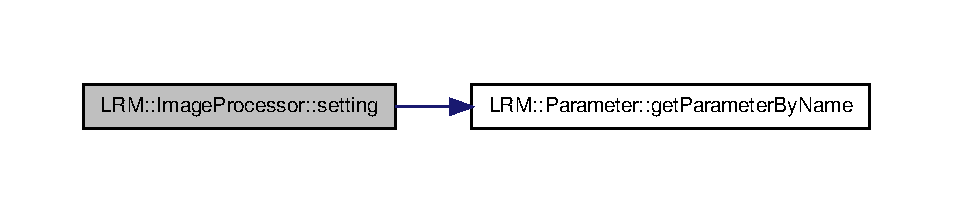
\includegraphics[width=350pt]{classLRM_1_1ImageProcessor_aa5ddc6b267ccb4afcb3871fc730f2c93_cgraph}
\end{center}
\end{figure}


\hypertarget{classLRM_1_1ImageProcessor_a8a8deb80b7824c5f0946acf1ff9df73e}{\index{\-L\-R\-M\-::\-Image\-Processor@{\-L\-R\-M\-::\-Image\-Processor}!\-Shi\-Tomasi\-Corner@{\-Shi\-Tomasi\-Corner}}
\index{\-Shi\-Tomasi\-Corner@{\-Shi\-Tomasi\-Corner}!LRM::ImageProcessor@{\-L\-R\-M\-::\-Image\-Processor}}
\subsubsection[{\-Shi\-Tomasi\-Corner}]{\setlength{\rightskip}{0pt plus 5cm}int {\bf \-L\-R\-M\-::\-Image\-Processor\-::\-Shi\-Tomasi\-Corner} (
\begin{DoxyParamCaption}
\item[{cv\-::\-Ptr$<$ cv\-::\-Feature\-Detector $>$}]{det, }
\item[{cv\-::\-Mat}]{src, }
\item[{std\-::vector$<$ cv\-::\-Key\-Point $>$ \&}]{array\-Of\-Features}
\end{DoxyParamCaption}
)\hspace{0.3cm}{\ttfamily  \mbox{[}static\mbox{]}}}}\label{classLRM_1_1ImageProcessor_a8a8deb80b7824c5f0946acf1ff9df73e}
\hypertarget{classLRM_1_1ImageProcessor_a175b94a0ed60b83d2b7687958d81193e}{\index{\-L\-R\-M\-::\-Image\-Processor@{\-L\-R\-M\-::\-Image\-Processor}!\-S\-U\-R\-F\-\_\-\-Detector@{\-S\-U\-R\-F\-\_\-\-Detector}}
\index{\-S\-U\-R\-F\-\_\-\-Detector@{\-S\-U\-R\-F\-\_\-\-Detector}!LRM::ImageProcessor@{\-L\-R\-M\-::\-Image\-Processor}}
\subsubsection[{\-S\-U\-R\-F\-\_\-\-Detector}]{\setlength{\rightskip}{0pt plus 5cm}int {\bf \-L\-R\-M\-::\-Image\-Processor\-::\-S\-U\-R\-F\-\_\-\-Detector} (
\begin{DoxyParamCaption}
\item[{cv\-::\-Ptr$<$ cv\-::\-Feature\-Detector $>$}]{det, }
\item[{cv\-::\-Mat}]{src, }
\item[{std\-::vector$<$ cv\-::\-Key\-Point $>$ \&}]{array\-Of\-Features}
\end{DoxyParamCaption}
)\hspace{0.3cm}{\ttfamily  \mbox{[}static\mbox{]}}}}\label{classLRM_1_1ImageProcessor_a175b94a0ed60b83d2b7687958d81193e}


\subsection{\-Member \-Data \-Documentation}
\hypertarget{classLRM_1_1ImageProcessor_a576a9af86d68d4394984e630c7ec452d}{\index{\-L\-R\-M\-::\-Image\-Processor@{\-L\-R\-M\-::\-Image\-Processor}!detector@{detector}}
\index{detector@{detector}!LRM::ImageProcessor@{\-L\-R\-M\-::\-Image\-Processor}}
\subsubsection[{detector}]{\setlength{\rightskip}{0pt plus 5cm}cv\-::\-Ptr$<$cv\-::\-Feature\-Detector$>$ {\bf \-L\-R\-M\-::\-Image\-Processor\-::detector}\hspace{0.3cm}{\ttfamily  \mbox{[}private\mbox{]}}}}\label{classLRM_1_1ImageProcessor_a576a9af86d68d4394984e630c7ec452d}
\hypertarget{classLRM_1_1ImageProcessor_a7a52a914f184c8b01fe42d582fc17af0}{\index{\-L\-R\-M\-::\-Image\-Processor@{\-L\-R\-M\-::\-Image\-Processor}!extractor@{extractor}}
\index{extractor@{extractor}!LRM::ImageProcessor@{\-L\-R\-M\-::\-Image\-Processor}}
\subsubsection[{extractor}]{\setlength{\rightskip}{0pt plus 5cm}cv\-::\-Ptr$<$cv\-::\-Descriptor\-Extractor$>$ {\bf \-L\-R\-M\-::\-Image\-Processor\-::extractor}\hspace{0.3cm}{\ttfamily  \mbox{[}private\mbox{]}}}}\label{classLRM_1_1ImageProcessor_a7a52a914f184c8b01fe42d582fc17af0}
\hypertarget{classLRM_1_1ImageProcessor_abdfb33d345e6e7eebff614252e27095b}{\index{\-L\-R\-M\-::\-Image\-Processor@{\-L\-R\-M\-::\-Image\-Processor}!feature\-\_\-type@{feature\-\_\-type}}
\index{feature\-\_\-type@{feature\-\_\-type}!LRM::ImageProcessor@{\-L\-R\-M\-::\-Image\-Processor}}
\subsubsection[{feature\-\_\-type}]{\setlength{\rightskip}{0pt plus 5cm}{\bf feature\-\_\-t} {\bf \-L\-R\-M\-::\-Image\-Processor\-::feature\-\_\-type}\hspace{0.3cm}{\ttfamily  \mbox{[}private\mbox{]}}}}\label{classLRM_1_1ImageProcessor_abdfb33d345e6e7eebff614252e27095b}
\hypertarget{classLRM_1_1ImageProcessor_a55350c39b33c45697fcf48ff75bef2d1}{\index{\-L\-R\-M\-::\-Image\-Processor@{\-L\-R\-M\-::\-Image\-Processor}!matcher@{matcher}}
\index{matcher@{matcher}!LRM::ImageProcessor@{\-L\-R\-M\-::\-Image\-Processor}}
\subsubsection[{matcher}]{\setlength{\rightskip}{0pt plus 5cm}cv\-::\-Ptr$<$cv\-::\-Descriptor\-Matcher$>$ {\bf \-L\-R\-M\-::\-Image\-Processor\-::matcher}\hspace{0.3cm}{\ttfamily  \mbox{[}private\mbox{]}}}}\label{classLRM_1_1ImageProcessor_a55350c39b33c45697fcf48ff75bef2d1}
\hypertarget{classLRM_1_1ImageProcessor_afcdba0a2c3377e8d89d8abb42632bf3a}{\index{\-L\-R\-M\-::\-Image\-Processor@{\-L\-R\-M\-::\-Image\-Processor}!max\-Number\-Of\-Features@{max\-Number\-Of\-Features}}
\index{max\-Number\-Of\-Features@{max\-Number\-Of\-Features}!LRM::ImageProcessor@{\-L\-R\-M\-::\-Image\-Processor}}
\subsubsection[{max\-Number\-Of\-Features}]{\setlength{\rightskip}{0pt plus 5cm}int {\bf \-L\-R\-M\-::\-Image\-Processor\-::max\-Number\-Of\-Features}\hspace{0.3cm}{\ttfamily  \mbox{[}private\mbox{]}}}}\label{classLRM_1_1ImageProcessor_afcdba0a2c3377e8d89d8abb42632bf3a}
\hypertarget{classLRM_1_1ImageProcessor_a46e10168106b028e29042dbe8e13f83e}{\index{\-L\-R\-M\-::\-Image\-Processor@{\-L\-R\-M\-::\-Image\-Processor}!radius@{radius}}
\index{radius@{radius}!LRM::ImageProcessor@{\-L\-R\-M\-::\-Image\-Processor}}
\subsubsection[{radius}]{\setlength{\rightskip}{0pt plus 5cm}double {\bf \-L\-R\-M\-::\-Image\-Processor\-::radius}\hspace{0.3cm}{\ttfamily  \mbox{[}private\mbox{]}}}}\label{classLRM_1_1ImageProcessor_a46e10168106b028e29042dbe8e13f83e}


\-The documentation for this class was generated from the following files\-:\begin{DoxyCompactItemize}
\item 
include/\hyperlink{image__processor_8h}{image\-\_\-processor.\-h}\item 
src/\hyperlink{image__processor_8cpp}{image\-\_\-processor.\-cpp}\end{DoxyCompactItemize}

\hypertarget{classLRM_1_1ImageProcessorParameter}{\section{\-L\-R\-M\-:\-:\-Image\-Processor\-Parameter \-Class \-Reference}
\label{classLRM_1_1ImageProcessorParameter}\index{\-L\-R\-M\-::\-Image\-Processor\-Parameter@{\-L\-R\-M\-::\-Image\-Processor\-Parameter}}
}


{\ttfamily \#include $<$image\-\_\-processor.\-h$>$}



\-Inheritance diagram for \-L\-R\-M\-:\-:\-Image\-Processor\-Parameter\-:\nopagebreak
\begin{figure}[H]
\begin{center}
\leavevmode
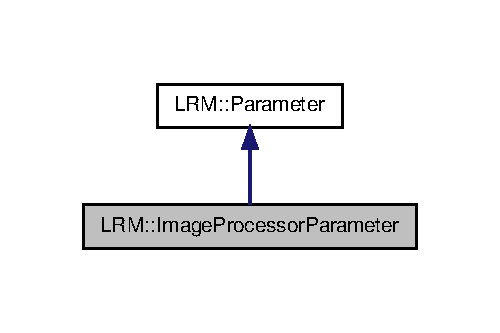
\includegraphics[width=240pt]{classLRM_1_1ImageProcessorParameter__inherit__graph}
\end{center}
\end{figure}


\-Collaboration diagram for \-L\-R\-M\-:\-:\-Image\-Processor\-Parameter\-:\nopagebreak
\begin{figure}[H]
\begin{center}
\leavevmode
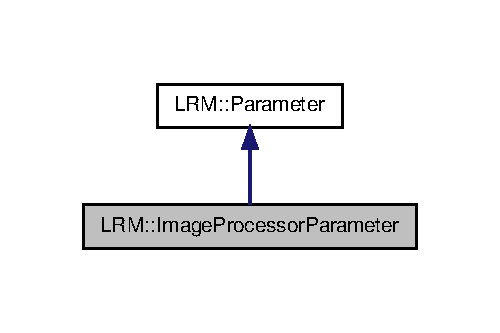
\includegraphics[width=240pt]{classLRM_1_1ImageProcessorParameter__coll__graph}
\end{center}
\end{figure}
\subsection*{\-Public \-Member \-Functions}
\begin{DoxyCompactItemize}
\item 
\hyperlink{classLRM_1_1ImageProcessorParameter_a83fe9807e1480dc000041f5c460b39af}{\-Image\-Processor\-Parameter} ()
\item 
\hyperlink{classLRM_1_1ImageProcessorParameter_ae384a255c8688ef911db3499a773c65b}{$\sim$\-Image\-Processor\-Parameter} ()
\item 
int \hyperlink{classLRM_1_1ImageProcessorParameter_a381448a39d6b41c8f44fd5b45f975b4a}{parse} (ros\-::\-Node\-Handle nh)
\end{DoxyCompactItemize}


\subsection{\-Detailed \-Description}
\-List of parameter regarding \-R\-O\-S configuration for the launch file.
\begin{DoxyItemize}
\item {\bfseries \-F\-E\-A\-T\-U\-R\-E\-\_\-\-T\-Y\-P\-E\-:} \-Type of feature to be detected. ({\bfseries \-Default\-:} \-S\-I\-F\-T)
\item {\bfseries \-M\-A\-X\-\_\-\-N\-U\-M\-\_\-\-F\-E\-A\-T\-U\-R\-E\-\_\-\-P\-T\-S\-:} \-Maximum number of features to be detected. ({\bfseries \-Default\-:} 100)
\item {\bfseries \-M\-A\-T\-C\-H\-\_\-\-R\-A\-D\-I\-U\-S\-:} \-Radius used as a filter for the feature match. ({\bfseries \-Default\-:} 10.\-0) 
\end{DoxyItemize}

\subsection{\-Constructor \& \-Destructor \-Documentation}
\hypertarget{classLRM_1_1ImageProcessorParameter_a83fe9807e1480dc000041f5c460b39af}{\index{\-L\-R\-M\-::\-Image\-Processor\-Parameter@{\-L\-R\-M\-::\-Image\-Processor\-Parameter}!\-Image\-Processor\-Parameter@{\-Image\-Processor\-Parameter}}
\index{\-Image\-Processor\-Parameter@{\-Image\-Processor\-Parameter}!LRM::ImageProcessorParameter@{\-L\-R\-M\-::\-Image\-Processor\-Parameter}}
\subsubsection[{\-Image\-Processor\-Parameter}]{\setlength{\rightskip}{0pt plus 5cm}{\bf \-L\-R\-M\-::\-Image\-Processor\-Parameter\-::\-Image\-Processor\-Parameter} (
\begin{DoxyParamCaption}
{}
\end{DoxyParamCaption}
)\hspace{0.3cm}{\ttfamily  \mbox{[}inline\mbox{]}}}}\label{classLRM_1_1ImageProcessorParameter_a83fe9807e1480dc000041f5c460b39af}
\hypertarget{classLRM_1_1ImageProcessorParameter_ae384a255c8688ef911db3499a773c65b}{\index{\-L\-R\-M\-::\-Image\-Processor\-Parameter@{\-L\-R\-M\-::\-Image\-Processor\-Parameter}!$\sim$\-Image\-Processor\-Parameter@{$\sim$\-Image\-Processor\-Parameter}}
\index{$\sim$\-Image\-Processor\-Parameter@{$\sim$\-Image\-Processor\-Parameter}!LRM::ImageProcessorParameter@{\-L\-R\-M\-::\-Image\-Processor\-Parameter}}
\subsubsection[{$\sim$\-Image\-Processor\-Parameter}]{\setlength{\rightskip}{0pt plus 5cm}{\bf \-L\-R\-M\-::\-Image\-Processor\-Parameter\-::$\sim$\-Image\-Processor\-Parameter} (
\begin{DoxyParamCaption}
{}
\end{DoxyParamCaption}
)\hspace{0.3cm}{\ttfamily  \mbox{[}inline\mbox{]}}}}\label{classLRM_1_1ImageProcessorParameter_ae384a255c8688ef911db3499a773c65b}


\subsection{\-Member \-Function \-Documentation}
\hypertarget{classLRM_1_1ImageProcessorParameter_a381448a39d6b41c8f44fd5b45f975b4a}{\index{\-L\-R\-M\-::\-Image\-Processor\-Parameter@{\-L\-R\-M\-::\-Image\-Processor\-Parameter}!parse@{parse}}
\index{parse@{parse}!LRM::ImageProcessorParameter@{\-L\-R\-M\-::\-Image\-Processor\-Parameter}}
\subsubsection[{parse}]{\setlength{\rightskip}{0pt plus 5cm}int {\bf \-L\-R\-M\-::\-Image\-Processor\-Parameter\-::parse} (
\begin{DoxyParamCaption}
\item[{ros\-::\-Node\-Handle}]{nh}
\end{DoxyParamCaption}
)\hspace{0.3cm}{\ttfamily  \mbox{[}virtual\mbox{]}}}}\label{classLRM_1_1ImageProcessorParameter_a381448a39d6b41c8f44fd5b45f975b4a}
\-Image \-Processor \hyperlink{classLRM_1_1Parameter}{\-Parameter} \-Class 

\-Implements \hyperlink{classLRM_1_1Parameter_ad53ef22f20e18578caa644866aaa234b}{\-L\-R\-M\-::\-Parameter}.



\-Here is the call graph for this function\-:\nopagebreak
\begin{figure}[H]
\begin{center}
\leavevmode
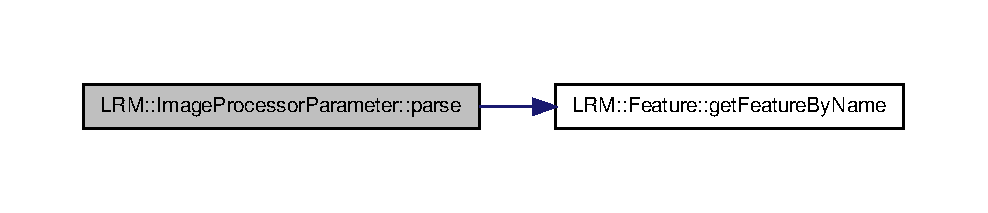
\includegraphics[width=350pt]{classLRM_1_1ImageProcessorParameter_a381448a39d6b41c8f44fd5b45f975b4a_cgraph}
\end{center}
\end{figure}




\-The documentation for this class was generated from the following files\-:\begin{DoxyCompactItemize}
\item 
include/\hyperlink{image__processor_8h}{image\-\_\-processor.\-h}\item 
src/\hyperlink{image__processor_8cpp}{image\-\_\-processor.\-cpp}\end{DoxyCompactItemize}

\hypertarget{classLRM_1_1MonoOdometer}{\section{\-L\-R\-M\-:\-:\-Mono\-Odometer \-Class \-Reference}
\label{classLRM_1_1MonoOdometer}\index{\-L\-R\-M\-::\-Mono\-Odometer@{\-L\-R\-M\-::\-Mono\-Odometer}}
}


{\ttfamily \#include $<$mono\-\_\-odometer.\-h$>$}



\-Collaboration diagram for \-L\-R\-M\-:\-:\-Mono\-Odometer\-:\nopagebreak
\begin{figure}[H]
\begin{center}
\leavevmode
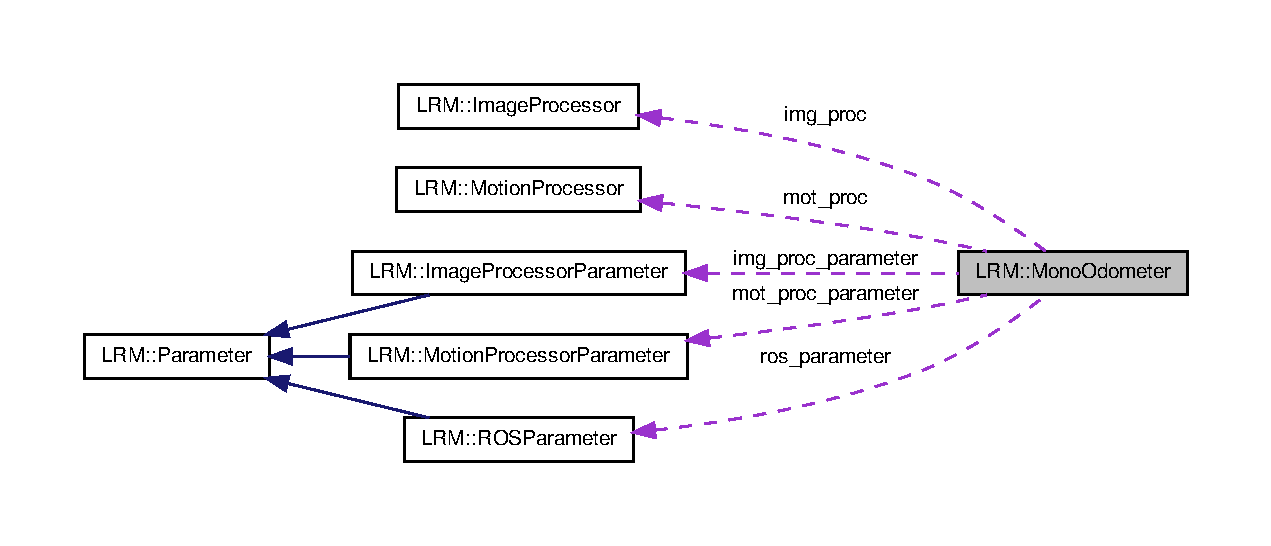
\includegraphics[width=350pt]{classLRM_1_1MonoOdometer__coll__graph}
\end{center}
\end{figure}
\subsection*{\-Public \-Member \-Functions}
\begin{DoxyCompactItemize}
\item 
\hyperlink{classLRM_1_1MonoOdometer_a1ea1f329885905fcab0e3f790253df9d}{\-Mono\-Odometer} ()
\item 
\hyperlink{classLRM_1_1MonoOdometer_ae849abdcd3e0b49be6b1672b292c86ba}{\-Mono\-Odometer} (ros\-::\-Node\-Handle \&nh, image\-\_\-transport\-::\-Image\-Transport \&it)
\begin{DoxyCompactList}\small\item\em \-The constructor of the \-Mono \-Odometer class. \-Captures and process a new frame and estimates the momentaneous motion. \end{DoxyCompactList}\item 
\hyperlink{classLRM_1_1MonoOdometer_aadca97effbd3970022f8fdfa42c1177b}{$\sim$\-Mono\-Odometer} ()
\item 
void \hyperlink{classLRM_1_1MonoOdometer_a7205e77893b1f9d4c37de616519ef5ed}{\-Image\-Callback} (const sensor\-\_\-msgs\-::\-Image\-Const\-Ptr \&msg)
\begin{DoxyCompactList}\small\item\em \-The \-Image \-Callback method is responsible for handling the income messages from the camera device and extract the frame features and descriptors. \end{DoxyCompactList}\item 
bool \hyperlink{classLRM_1_1MonoOdometer_aaea86d0c2fc1119b066b310451be4a67}{is\-Intrinsic\-Matrix\-Path} ()
\item 
std\-::string \hyperlink{classLRM_1_1MonoOdometer_ab75736159a13ba537ed8615c84853243}{get\-Intrinsic\-Matrix\-Path} ()
\item 
std\-::string \hyperlink{classLRM_1_1MonoOdometer_a3174620fdca5f375ec38bc0709c2e1e0}{get\-Input\-Image\-Topic} ()
\item 
std\-::string \hyperlink{classLRM_1_1MonoOdometer_a68f5f4b33141cd2a2ea92db6197db65c}{get\-Feature\-Image\-Topic} ()
\item 
std\-::string \hyperlink{classLRM_1_1MonoOdometer_a0b5b603776c1c011d1268dc029dee6ae}{get\-Matches\-Image\-Topic} ()
\item 
std\-::string \hyperlink{classLRM_1_1MonoOdometer_acde0fd05b19f524bace7c71de9a0cc36}{get\-Opt\-Flow\-Image\-Topic} ()
\item 
std\-::string \hyperlink{classLRM_1_1MonoOdometer_a16eaa3716cb077ef993fa66a582fe65e}{get\-Odometry\-Topic} ()
\item 
std\-::string \hyperlink{classLRM_1_1MonoOdometer_ac989d0a61c0b18c7e538732668953fa1}{get\-Odometer\-Reference\-Frame} ()
\item 
std\-::string \hyperlink{classLRM_1_1MonoOdometer_a3550a896dd2e212fa177d7401f1a5b61}{get\-Robot\-Frame} ()
\item 
std\-::string \hyperlink{classLRM_1_1MonoOdometer_a72b47de741d2c273a34c7d4e9a093092}{get\-Sensor\-Frame} ()
\end{DoxyCompactItemize}
\subsection*{\-Private \-Member \-Functions}
\begin{DoxyCompactItemize}
\item 
int \hyperlink{classLRM_1_1MonoOdometer_a8c7914efde9c07323c171d7adfaf656e}{update\-\_\-pose} ()
\item 
int \hyperlink{classLRM_1_1MonoOdometer_ab33c598738d4c565cae80ca110f3ab63}{convert\-Sensor\-Msg\-To\-Image} (const sensor\-\_\-msgs\-::\-Image\-Const\-Ptr \&msg, cv\-\_\-bridge\-::\-Cv\-Image\-Const\-Ptr \&image)
\begin{DoxyCompactList}\small\item\em \-Converts a sensor message to a grayscale image. \end{DoxyCompactList}\item 
int \hyperlink{classLRM_1_1MonoOdometer_acdfde454162a9fba808c5e99069e5831}{draw\-Feature\-Image} ()
\item 
int \hyperlink{classLRM_1_1MonoOdometer_a0e648fa164c12e1bb405c5e0de9607cf}{draw\-Matches\-Image} ()
\item 
int \hyperlink{classLRM_1_1MonoOdometer_ac3e11ffd664dfd8b06068f77dd475ed4}{draw\-Opt\-Flow\-Image} ()
\end{DoxyCompactItemize}
\subsection*{\-Private \-Attributes}
\begin{DoxyCompactItemize}
\item 
ros\-::\-Time \hyperlink{classLRM_1_1MonoOdometer_ae201ba1988badf708c046e1b29b70ab1}{query\-\_\-timestamp}
\item 
ros\-::\-Time \hyperlink{classLRM_1_1MonoOdometer_a7024b12b516c41771d59046471ea7319}{train\-\_\-timestamp}
\item 
cv\-::\-Mat \hyperlink{classLRM_1_1MonoOdometer_a7f874bb9b174d7a38085782377d5f195}{\-K}
\item 
\hyperlink{classLRM_1_1ROSParameter}{\-R\-O\-S\-Parameter} \hyperlink{classLRM_1_1MonoOdometer_a7667abb4e8d035e25811c63e6af42ae3}{ros\-\_\-parameter}
\item 
image\-\_\-transport\-::\-Subscriber \hyperlink{classLRM_1_1MonoOdometer_ad191c12993c8e8ee9200f71aec07057c}{input\-\_\-image\-\_\-subscriber}
\item 
image\-\_\-transport\-::\-Publisher \hyperlink{classLRM_1_1MonoOdometer_abcc8b0e66d3629d66b74e8d857adea9e}{output\-\_\-feature\-\_\-advertiser}
\item 
image\-\_\-transport\-::\-Publisher \hyperlink{classLRM_1_1MonoOdometer_ab3e372106292ea873dc5428e1b3d0026}{output\-\_\-matches\-\_\-advertiser}
\item 
image\-\_\-transport\-::\-Publisher \hyperlink{classLRM_1_1MonoOdometer_a2f9dcb6ceed7b4b85e0df512fc297105}{output\-\_\-optflow\-\_\-advertiser}
\item 
ros\-::\-Publisher \hyperlink{classLRM_1_1MonoOdometer_a113a9a4905bb7c9f19df55610802ffec}{odometry\-\_\-advertiser}
\item 
\hyperlink{classLRM_1_1ImageProcessor}{\-Image\-Processor} \hyperlink{classLRM_1_1MonoOdometer_a49bef96a5413beea489f87dbb16eaf70}{img\-\_\-proc}
\item 
\hyperlink{classLRM_1_1ImageProcessorParameter}{\-Image\-Processor\-Parameter} \hyperlink{classLRM_1_1MonoOdometer_a1bf24a1abdef05b79b54813058cad4a7}{img\-\_\-proc\-\_\-parameter}
\item 
cv\-\_\-bridge\-::\-Cv\-Image\-Const\-Ptr \hyperlink{classLRM_1_1MonoOdometer_a91ee6e52006559ba0f769a2ccc06fa64}{train\-\_\-image}
\begin{DoxyCompactList}\small\item\em \-Previous image. \end{DoxyCompactList}\item 
cv\-\_\-bridge\-::\-Cv\-Image\-Const\-Ptr \hyperlink{classLRM_1_1MonoOdometer_a1fbec0b090c10b1c542bd86f18795a14}{query\-\_\-image}
\begin{DoxyCompactList}\small\item\em \-Current image. \end{DoxyCompactList}\item 
cv\-\_\-bridge\-::\-Cv\-Image \hyperlink{classLRM_1_1MonoOdometer_a166844b373399a94d688234592ae8468}{feature\-\_\-image}
\item 
cv\-\_\-bridge\-::\-Cv\-Image \hyperlink{classLRM_1_1MonoOdometer_a1646743b51e5e0386def055e0265aaf2}{matches\-\_\-image}
\item 
cv\-\_\-bridge\-::\-Cv\-Image \hyperlink{classLRM_1_1MonoOdometer_a5f9b4ef57cf2b7d88bb92c8269a8792d}{optflow\-\_\-image}
\item 
std\-::vector$<$ cv\-::\-Key\-Point $>$ \hyperlink{classLRM_1_1MonoOdometer_a98515916ee97beaefb9bbcf07cd02d1b}{train\-\_\-kpts}
\begin{DoxyCompactList}\small\item\em \-Previous image keypoints. \end{DoxyCompactList}\item 
std\-::vector$<$ cv\-::\-Key\-Point $>$ \hyperlink{classLRM_1_1MonoOdometer_a18d64f992353bf50e1421a1cb9ca32f2}{query\-\_\-kpts}
\begin{DoxyCompactList}\small\item\em \-Current image keypoints. \end{DoxyCompactList}\item 
std\-::vector$<$ cv\-::\-Point2d $>$ \hyperlink{classLRM_1_1MonoOdometer_accbdc3f32cf2fb8e75f3f40cd8a4e60e}{train\-\_\-pts}
\item 
std\-::vector$<$ cv\-::\-Point2d $>$ \hyperlink{classLRM_1_1MonoOdometer_a4d269a8b3827580e73515e8f958e2283}{query\-\_\-pts}
\item 
cv\-::\-Mat \hyperlink{classLRM_1_1MonoOdometer_aae6c2096b1b0c785548bc57cf6557427}{train\-\_\-desc}
\item 
cv\-::\-Mat \hyperlink{classLRM_1_1MonoOdometer_a7bf26df30d6cebf7e6c5b85c2318ff51}{query\-\_\-desc}
\item 
std\-::vector$<$ cv\-::\-D\-Match $>$ \hyperlink{classLRM_1_1MonoOdometer_aefc5720615c86208707622253d2e08ed}{matches}
\item 
\hyperlink{classLRM_1_1MotionProcessor}{\-Motion\-Processor} \hyperlink{classLRM_1_1MonoOdometer_a91b2fd9ac3051a11e7008c2e3740a382}{mot\-\_\-proc}
\item 
\hyperlink{classLRM_1_1MotionProcessorParameter}{\-Motion\-Processor\-Parameter} \hyperlink{classLRM_1_1MonoOdometer_a8bf0ca69100b032fe3c73fb1e0bed318}{mot\-\_\-proc\-\_\-parameter}
\item 
tf\-::\-Transform \hyperlink{classLRM_1_1MonoOdometer_a086c208e839df4586e99d417c60a3d77}{pose}
\item 
tf\-::\-Stamped\-Transform \hyperlink{classLRM_1_1MonoOdometer_a311831c9328491cde059e17706fd9bdc}{base\-\_\-to\-\_\-sensor}
\item 
tf\-::\-Transform\-Broadcaster \hyperlink{classLRM_1_1MonoOdometer_a85bf06a46a0367a821f145e1c3f51e8c}{odom\-\_\-broadcaster}
\item 
tf\-::\-Transform\-Listener \hyperlink{classLRM_1_1MonoOdometer_aa17423bfec7b2a995672d40cc6ed4fbe}{tf\-\_\-listener}
\item 
nav\-\_\-msgs\-::\-Odometry \hyperlink{classLRM_1_1MonoOdometer_afdc33ed78a3234b3469e094b23b4d511}{odometry}
\end{DoxyCompactItemize}


\subsection{\-Constructor \& \-Destructor \-Documentation}
\hypertarget{classLRM_1_1MonoOdometer_a1ea1f329885905fcab0e3f790253df9d}{\index{\-L\-R\-M\-::\-Mono\-Odometer@{\-L\-R\-M\-::\-Mono\-Odometer}!\-Mono\-Odometer@{\-Mono\-Odometer}}
\index{\-Mono\-Odometer@{\-Mono\-Odometer}!LRM::MonoOdometer@{\-L\-R\-M\-::\-Mono\-Odometer}}
\subsubsection[{\-Mono\-Odometer}]{\setlength{\rightskip}{0pt plus 5cm}{\bf \-L\-R\-M\-::\-Mono\-Odometer\-::\-Mono\-Odometer} (
\begin{DoxyParamCaption}
{}
\end{DoxyParamCaption}
)}}\label{classLRM_1_1MonoOdometer_a1ea1f329885905fcab0e3f790253df9d}
\hyperlink{classLRM_1_1MonoOdometer}{\-Mono\-Odometer} \-Class \hypertarget{classLRM_1_1MonoOdometer_ae849abdcd3e0b49be6b1672b292c86ba}{\index{\-L\-R\-M\-::\-Mono\-Odometer@{\-L\-R\-M\-::\-Mono\-Odometer}!\-Mono\-Odometer@{\-Mono\-Odometer}}
\index{\-Mono\-Odometer@{\-Mono\-Odometer}!LRM::MonoOdometer@{\-L\-R\-M\-::\-Mono\-Odometer}}
\subsubsection[{\-Mono\-Odometer}]{\setlength{\rightskip}{0pt plus 5cm}{\bf \-L\-R\-M\-::\-Mono\-Odometer\-::\-Mono\-Odometer} (
\begin{DoxyParamCaption}
\item[{ros\-::\-Node\-Handle \&}]{nh, }
\item[{image\-\_\-transport\-::\-Image\-Transport \&}]{it}
\end{DoxyParamCaption}
)}}\label{classLRM_1_1MonoOdometer_ae849abdcd3e0b49be6b1672b292c86ba}


\-The constructor of the \-Mono \-Odometer class. \-Captures and process a new frame and estimates the momentaneous motion. 


\begin{DoxyParams}[1]{\-Parameters}
\mbox{\tt in}  & {\em nh} & \-Node handle of the node of the monocular odometer. \\
\hline
\mbox{\tt in}  & {\em it} & \-Image transport handler. \\
\hline
\end{DoxyParams}


\-Here is the call graph for this function\-:\nopagebreak
\begin{figure}[H]
\begin{center}
\leavevmode
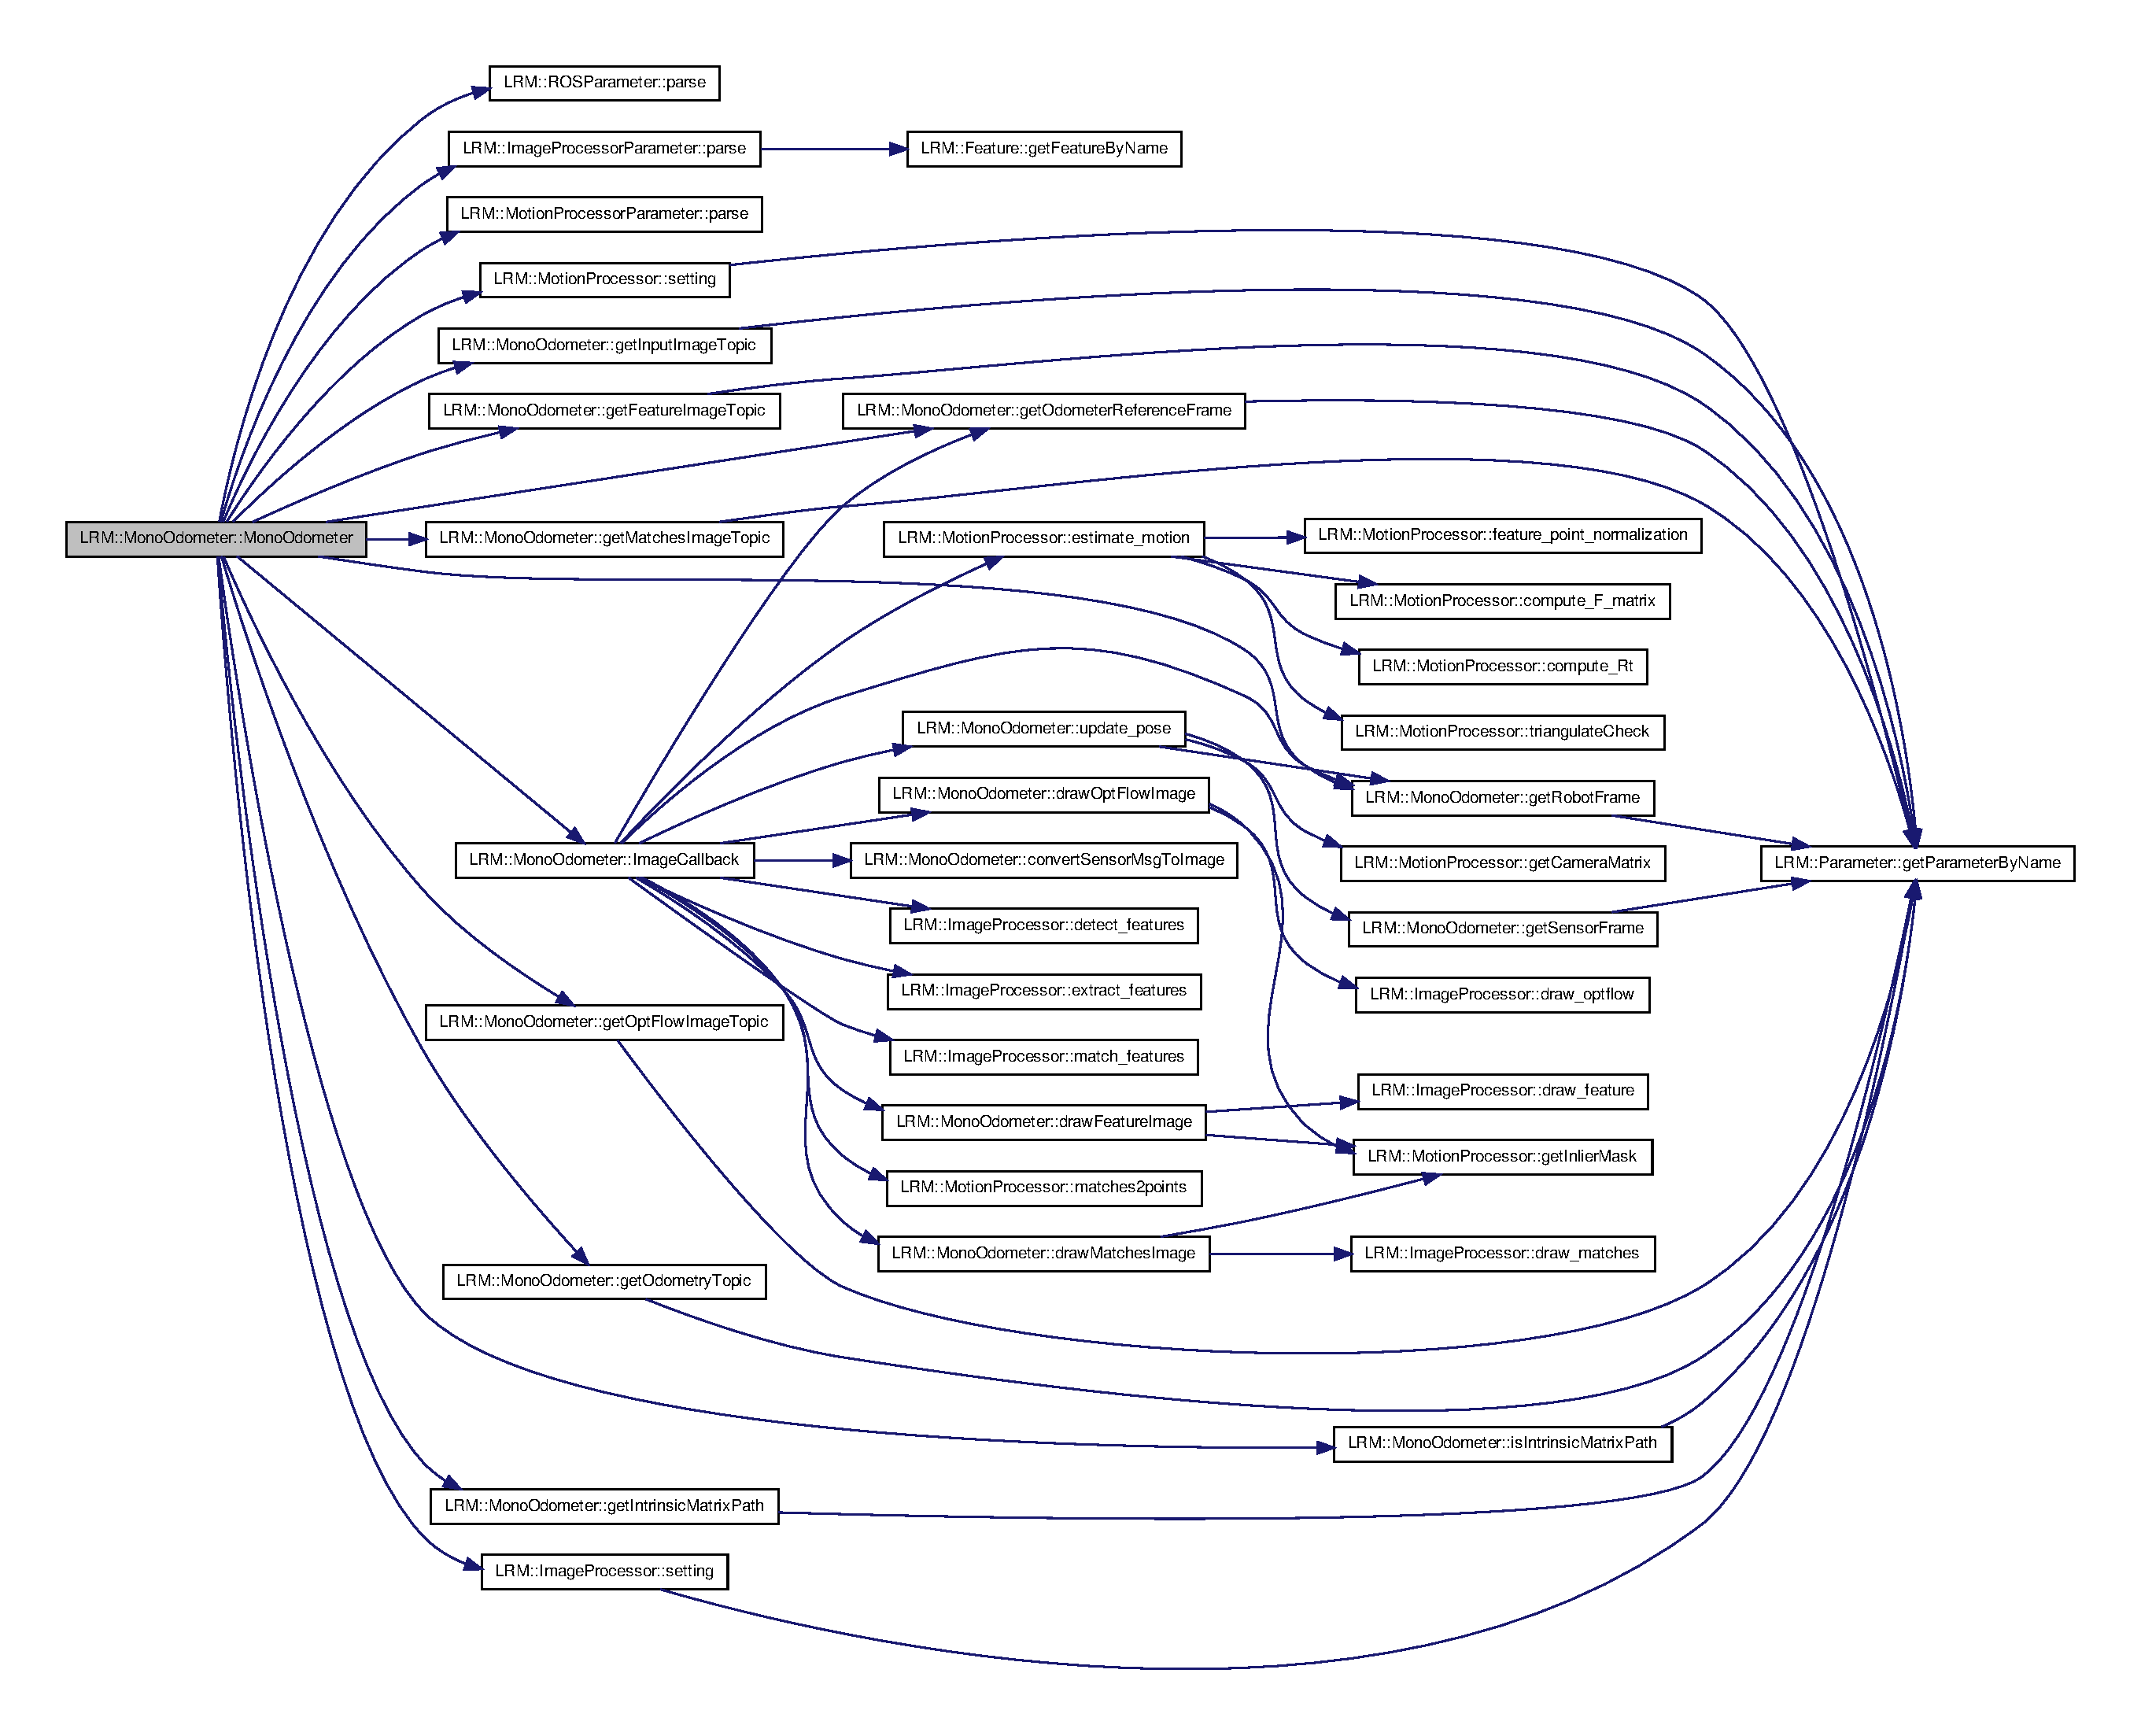
\includegraphics[width=350pt]{classLRM_1_1MonoOdometer_ae849abdcd3e0b49be6b1672b292c86ba_cgraph}
\end{center}
\end{figure}


\hypertarget{classLRM_1_1MonoOdometer_aadca97effbd3970022f8fdfa42c1177b}{\index{\-L\-R\-M\-::\-Mono\-Odometer@{\-L\-R\-M\-::\-Mono\-Odometer}!$\sim$\-Mono\-Odometer@{$\sim$\-Mono\-Odometer}}
\index{$\sim$\-Mono\-Odometer@{$\sim$\-Mono\-Odometer}!LRM::MonoOdometer@{\-L\-R\-M\-::\-Mono\-Odometer}}
\subsubsection[{$\sim$\-Mono\-Odometer}]{\setlength{\rightskip}{0pt plus 5cm}{\bf \-L\-R\-M\-::\-Mono\-Odometer\-::$\sim$\-Mono\-Odometer} (
\begin{DoxyParamCaption}
{}
\end{DoxyParamCaption}
)}}\label{classLRM_1_1MonoOdometer_aadca97effbd3970022f8fdfa42c1177b}


\subsection{\-Member \-Function \-Documentation}
\hypertarget{classLRM_1_1MonoOdometer_ab33c598738d4c565cae80ca110f3ab63}{\index{\-L\-R\-M\-::\-Mono\-Odometer@{\-L\-R\-M\-::\-Mono\-Odometer}!convert\-Sensor\-Msg\-To\-Image@{convert\-Sensor\-Msg\-To\-Image}}
\index{convert\-Sensor\-Msg\-To\-Image@{convert\-Sensor\-Msg\-To\-Image}!LRM::MonoOdometer@{\-L\-R\-M\-::\-Mono\-Odometer}}
\subsubsection[{convert\-Sensor\-Msg\-To\-Image}]{\setlength{\rightskip}{0pt plus 5cm}int {\bf \-L\-R\-M\-::\-Mono\-Odometer\-::convert\-Sensor\-Msg\-To\-Image} (
\begin{DoxyParamCaption}
\item[{const sensor\-\_\-msgs\-::\-Image\-Const\-Ptr \&}]{msg, }
\item[{cv\-\_\-bridge\-::\-Cv\-Image\-Const\-Ptr \&}]{image}
\end{DoxyParamCaption}
)\hspace{0.3cm}{\ttfamily  \mbox{[}private\mbox{]}}}}\label{classLRM_1_1MonoOdometer_ab33c598738d4c565cae80ca110f3ab63}


\-Converts a sensor message to a grayscale image. 


\begin{DoxyParams}{\-Parameters}
{\em msg} & \-Sensor image \\
\hline
{\em image} & \-Output image \\
\hline
\end{DoxyParams}
\begin{DoxyReturn}{\-Returns}
\-Error code 
\end{DoxyReturn}
\hypertarget{classLRM_1_1MonoOdometer_acdfde454162a9fba808c5e99069e5831}{\index{\-L\-R\-M\-::\-Mono\-Odometer@{\-L\-R\-M\-::\-Mono\-Odometer}!draw\-Feature\-Image@{draw\-Feature\-Image}}
\index{draw\-Feature\-Image@{draw\-Feature\-Image}!LRM::MonoOdometer@{\-L\-R\-M\-::\-Mono\-Odometer}}
\subsubsection[{draw\-Feature\-Image}]{\setlength{\rightskip}{0pt plus 5cm}int {\bf \-L\-R\-M\-::\-Mono\-Odometer\-::draw\-Feature\-Image} (
\begin{DoxyParamCaption}
{}
\end{DoxyParamCaption}
)\hspace{0.3cm}{\ttfamily  \mbox{[}private\mbox{]}}}}\label{classLRM_1_1MonoOdometer_acdfde454162a9fba808c5e99069e5831}


\-Here is the call graph for this function\-:\nopagebreak
\begin{figure}[H]
\begin{center}
\leavevmode
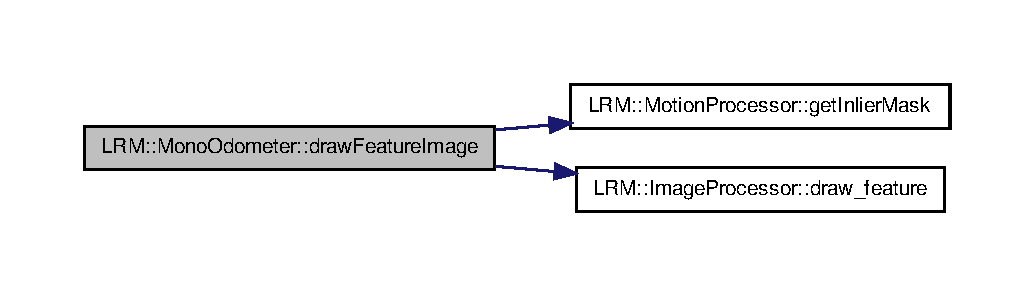
\includegraphics[width=350pt]{classLRM_1_1MonoOdometer_acdfde454162a9fba808c5e99069e5831_cgraph}
\end{center}
\end{figure}


\hypertarget{classLRM_1_1MonoOdometer_a0e648fa164c12e1bb405c5e0de9607cf}{\index{\-L\-R\-M\-::\-Mono\-Odometer@{\-L\-R\-M\-::\-Mono\-Odometer}!draw\-Matches\-Image@{draw\-Matches\-Image}}
\index{draw\-Matches\-Image@{draw\-Matches\-Image}!LRM::MonoOdometer@{\-L\-R\-M\-::\-Mono\-Odometer}}
\subsubsection[{draw\-Matches\-Image}]{\setlength{\rightskip}{0pt plus 5cm}int {\bf \-L\-R\-M\-::\-Mono\-Odometer\-::draw\-Matches\-Image} (
\begin{DoxyParamCaption}
{}
\end{DoxyParamCaption}
)\hspace{0.3cm}{\ttfamily  \mbox{[}private\mbox{]}}}}\label{classLRM_1_1MonoOdometer_a0e648fa164c12e1bb405c5e0de9607cf}


\-Here is the call graph for this function\-:\nopagebreak
\begin{figure}[H]
\begin{center}
\leavevmode
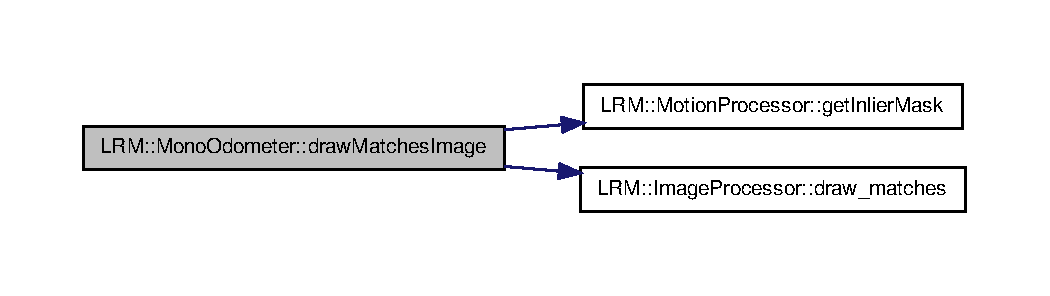
\includegraphics[width=350pt]{classLRM_1_1MonoOdometer_a0e648fa164c12e1bb405c5e0de9607cf_cgraph}
\end{center}
\end{figure}


\hypertarget{classLRM_1_1MonoOdometer_ac3e11ffd664dfd8b06068f77dd475ed4}{\index{\-L\-R\-M\-::\-Mono\-Odometer@{\-L\-R\-M\-::\-Mono\-Odometer}!draw\-Opt\-Flow\-Image@{draw\-Opt\-Flow\-Image}}
\index{draw\-Opt\-Flow\-Image@{draw\-Opt\-Flow\-Image}!LRM::MonoOdometer@{\-L\-R\-M\-::\-Mono\-Odometer}}
\subsubsection[{draw\-Opt\-Flow\-Image}]{\setlength{\rightskip}{0pt plus 5cm}int {\bf \-L\-R\-M\-::\-Mono\-Odometer\-::draw\-Opt\-Flow\-Image} (
\begin{DoxyParamCaption}
{}
\end{DoxyParamCaption}
)\hspace{0.3cm}{\ttfamily  \mbox{[}private\mbox{]}}}}\label{classLRM_1_1MonoOdometer_ac3e11ffd664dfd8b06068f77dd475ed4}


\-Here is the call graph for this function\-:\nopagebreak
\begin{figure}[H]
\begin{center}
\leavevmode
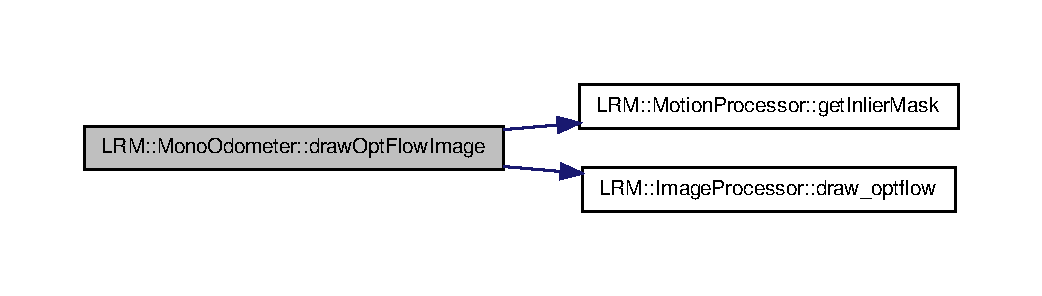
\includegraphics[width=350pt]{classLRM_1_1MonoOdometer_ac3e11ffd664dfd8b06068f77dd475ed4_cgraph}
\end{center}
\end{figure}


\hypertarget{classLRM_1_1MonoOdometer_a68f5f4b33141cd2a2ea92db6197db65c}{\index{\-L\-R\-M\-::\-Mono\-Odometer@{\-L\-R\-M\-::\-Mono\-Odometer}!get\-Feature\-Image\-Topic@{get\-Feature\-Image\-Topic}}
\index{get\-Feature\-Image\-Topic@{get\-Feature\-Image\-Topic}!LRM::MonoOdometer@{\-L\-R\-M\-::\-Mono\-Odometer}}
\subsubsection[{get\-Feature\-Image\-Topic}]{\setlength{\rightskip}{0pt plus 5cm}std\-::string {\bf \-L\-R\-M\-::\-Mono\-Odometer\-::get\-Feature\-Image\-Topic} (
\begin{DoxyParamCaption}
{}
\end{DoxyParamCaption}
)\hspace{0.3cm}{\ttfamily  \mbox{[}inline\mbox{]}}}}\label{classLRM_1_1MonoOdometer_a68f5f4b33141cd2a2ea92db6197db65c}


\-Here is the call graph for this function\-:\nopagebreak
\begin{figure}[H]
\begin{center}
\leavevmode
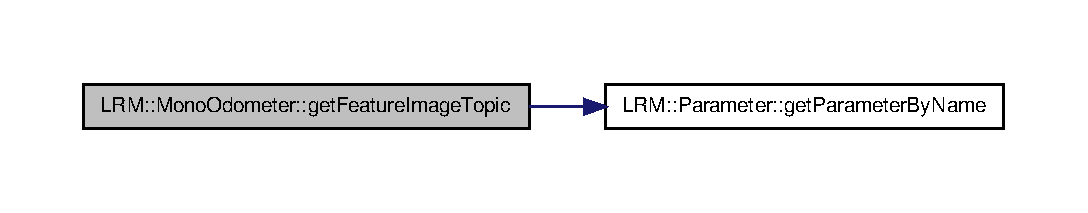
\includegraphics[width=350pt]{classLRM_1_1MonoOdometer_a68f5f4b33141cd2a2ea92db6197db65c_cgraph}
\end{center}
\end{figure}


\hypertarget{classLRM_1_1MonoOdometer_a3174620fdca5f375ec38bc0709c2e1e0}{\index{\-L\-R\-M\-::\-Mono\-Odometer@{\-L\-R\-M\-::\-Mono\-Odometer}!get\-Input\-Image\-Topic@{get\-Input\-Image\-Topic}}
\index{get\-Input\-Image\-Topic@{get\-Input\-Image\-Topic}!LRM::MonoOdometer@{\-L\-R\-M\-::\-Mono\-Odometer}}
\subsubsection[{get\-Input\-Image\-Topic}]{\setlength{\rightskip}{0pt plus 5cm}std\-::string {\bf \-L\-R\-M\-::\-Mono\-Odometer\-::get\-Input\-Image\-Topic} (
\begin{DoxyParamCaption}
{}
\end{DoxyParamCaption}
)\hspace{0.3cm}{\ttfamily  \mbox{[}inline\mbox{]}}}}\label{classLRM_1_1MonoOdometer_a3174620fdca5f375ec38bc0709c2e1e0}


\-Here is the call graph for this function\-:\nopagebreak
\begin{figure}[H]
\begin{center}
\leavevmode
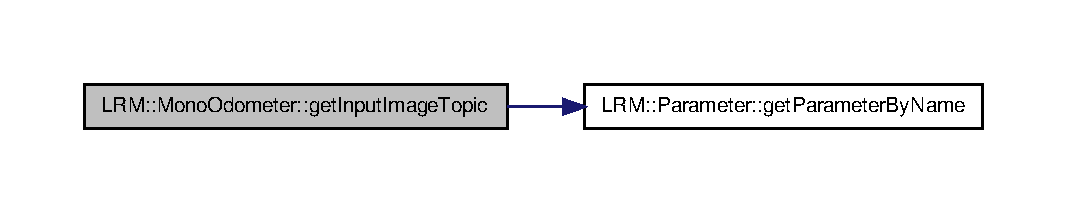
\includegraphics[width=350pt]{classLRM_1_1MonoOdometer_a3174620fdca5f375ec38bc0709c2e1e0_cgraph}
\end{center}
\end{figure}


\hypertarget{classLRM_1_1MonoOdometer_ab75736159a13ba537ed8615c84853243}{\index{\-L\-R\-M\-::\-Mono\-Odometer@{\-L\-R\-M\-::\-Mono\-Odometer}!get\-Intrinsic\-Matrix\-Path@{get\-Intrinsic\-Matrix\-Path}}
\index{get\-Intrinsic\-Matrix\-Path@{get\-Intrinsic\-Matrix\-Path}!LRM::MonoOdometer@{\-L\-R\-M\-::\-Mono\-Odometer}}
\subsubsection[{get\-Intrinsic\-Matrix\-Path}]{\setlength{\rightskip}{0pt plus 5cm}std\-::string {\bf \-L\-R\-M\-::\-Mono\-Odometer\-::get\-Intrinsic\-Matrix\-Path} (
\begin{DoxyParamCaption}
{}
\end{DoxyParamCaption}
)\hspace{0.3cm}{\ttfamily  \mbox{[}inline\mbox{]}}}}\label{classLRM_1_1MonoOdometer_ab75736159a13ba537ed8615c84853243}


\-Here is the call graph for this function\-:\nopagebreak
\begin{figure}[H]
\begin{center}
\leavevmode
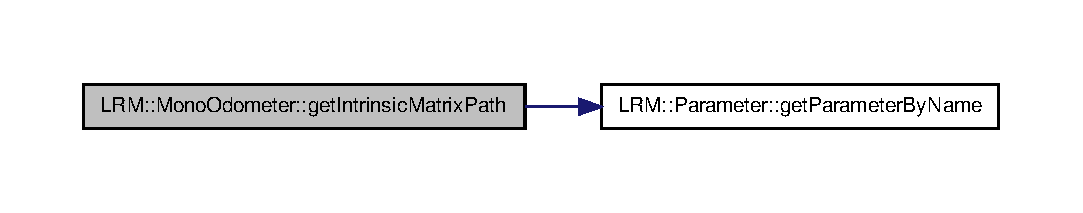
\includegraphics[width=350pt]{classLRM_1_1MonoOdometer_ab75736159a13ba537ed8615c84853243_cgraph}
\end{center}
\end{figure}


\hypertarget{classLRM_1_1MonoOdometer_a0b5b603776c1c011d1268dc029dee6ae}{\index{\-L\-R\-M\-::\-Mono\-Odometer@{\-L\-R\-M\-::\-Mono\-Odometer}!get\-Matches\-Image\-Topic@{get\-Matches\-Image\-Topic}}
\index{get\-Matches\-Image\-Topic@{get\-Matches\-Image\-Topic}!LRM::MonoOdometer@{\-L\-R\-M\-::\-Mono\-Odometer}}
\subsubsection[{get\-Matches\-Image\-Topic}]{\setlength{\rightskip}{0pt plus 5cm}std\-::string {\bf \-L\-R\-M\-::\-Mono\-Odometer\-::get\-Matches\-Image\-Topic} (
\begin{DoxyParamCaption}
{}
\end{DoxyParamCaption}
)\hspace{0.3cm}{\ttfamily  \mbox{[}inline\mbox{]}}}}\label{classLRM_1_1MonoOdometer_a0b5b603776c1c011d1268dc029dee6ae}


\-Here is the call graph for this function\-:\nopagebreak
\begin{figure}[H]
\begin{center}
\leavevmode
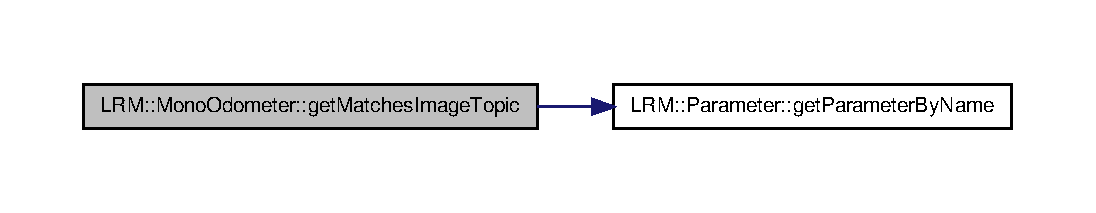
\includegraphics[width=350pt]{classLRM_1_1MonoOdometer_a0b5b603776c1c011d1268dc029dee6ae_cgraph}
\end{center}
\end{figure}


\hypertarget{classLRM_1_1MonoOdometer_ac989d0a61c0b18c7e538732668953fa1}{\index{\-L\-R\-M\-::\-Mono\-Odometer@{\-L\-R\-M\-::\-Mono\-Odometer}!get\-Odometer\-Reference\-Frame@{get\-Odometer\-Reference\-Frame}}
\index{get\-Odometer\-Reference\-Frame@{get\-Odometer\-Reference\-Frame}!LRM::MonoOdometer@{\-L\-R\-M\-::\-Mono\-Odometer}}
\subsubsection[{get\-Odometer\-Reference\-Frame}]{\setlength{\rightskip}{0pt plus 5cm}std\-::string {\bf \-L\-R\-M\-::\-Mono\-Odometer\-::get\-Odometer\-Reference\-Frame} (
\begin{DoxyParamCaption}
{}
\end{DoxyParamCaption}
)\hspace{0.3cm}{\ttfamily  \mbox{[}inline\mbox{]}}}}\label{classLRM_1_1MonoOdometer_ac989d0a61c0b18c7e538732668953fa1}


\-Here is the call graph for this function\-:\nopagebreak
\begin{figure}[H]
\begin{center}
\leavevmode
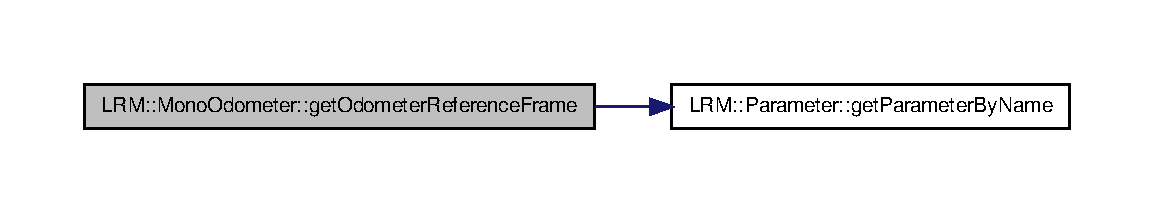
\includegraphics[width=350pt]{classLRM_1_1MonoOdometer_ac989d0a61c0b18c7e538732668953fa1_cgraph}
\end{center}
\end{figure}


\hypertarget{classLRM_1_1MonoOdometer_a16eaa3716cb077ef993fa66a582fe65e}{\index{\-L\-R\-M\-::\-Mono\-Odometer@{\-L\-R\-M\-::\-Mono\-Odometer}!get\-Odometry\-Topic@{get\-Odometry\-Topic}}
\index{get\-Odometry\-Topic@{get\-Odometry\-Topic}!LRM::MonoOdometer@{\-L\-R\-M\-::\-Mono\-Odometer}}
\subsubsection[{get\-Odometry\-Topic}]{\setlength{\rightskip}{0pt plus 5cm}std\-::string {\bf \-L\-R\-M\-::\-Mono\-Odometer\-::get\-Odometry\-Topic} (
\begin{DoxyParamCaption}
{}
\end{DoxyParamCaption}
)\hspace{0.3cm}{\ttfamily  \mbox{[}inline\mbox{]}}}}\label{classLRM_1_1MonoOdometer_a16eaa3716cb077ef993fa66a582fe65e}


\-Here is the call graph for this function\-:\nopagebreak
\begin{figure}[H]
\begin{center}
\leavevmode
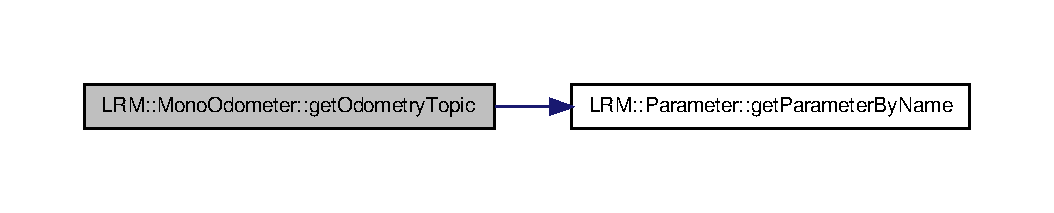
\includegraphics[width=350pt]{classLRM_1_1MonoOdometer_a16eaa3716cb077ef993fa66a582fe65e_cgraph}
\end{center}
\end{figure}


\hypertarget{classLRM_1_1MonoOdometer_acde0fd05b19f524bace7c71de9a0cc36}{\index{\-L\-R\-M\-::\-Mono\-Odometer@{\-L\-R\-M\-::\-Mono\-Odometer}!get\-Opt\-Flow\-Image\-Topic@{get\-Opt\-Flow\-Image\-Topic}}
\index{get\-Opt\-Flow\-Image\-Topic@{get\-Opt\-Flow\-Image\-Topic}!LRM::MonoOdometer@{\-L\-R\-M\-::\-Mono\-Odometer}}
\subsubsection[{get\-Opt\-Flow\-Image\-Topic}]{\setlength{\rightskip}{0pt plus 5cm}std\-::string {\bf \-L\-R\-M\-::\-Mono\-Odometer\-::get\-Opt\-Flow\-Image\-Topic} (
\begin{DoxyParamCaption}
{}
\end{DoxyParamCaption}
)\hspace{0.3cm}{\ttfamily  \mbox{[}inline\mbox{]}}}}\label{classLRM_1_1MonoOdometer_acde0fd05b19f524bace7c71de9a0cc36}


\-Here is the call graph for this function\-:\nopagebreak
\begin{figure}[H]
\begin{center}
\leavevmode
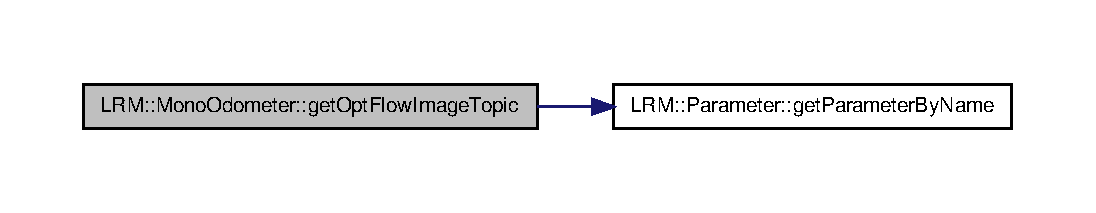
\includegraphics[width=350pt]{classLRM_1_1MonoOdometer_acde0fd05b19f524bace7c71de9a0cc36_cgraph}
\end{center}
\end{figure}


\hypertarget{classLRM_1_1MonoOdometer_a3550a896dd2e212fa177d7401f1a5b61}{\index{\-L\-R\-M\-::\-Mono\-Odometer@{\-L\-R\-M\-::\-Mono\-Odometer}!get\-Robot\-Frame@{get\-Robot\-Frame}}
\index{get\-Robot\-Frame@{get\-Robot\-Frame}!LRM::MonoOdometer@{\-L\-R\-M\-::\-Mono\-Odometer}}
\subsubsection[{get\-Robot\-Frame}]{\setlength{\rightskip}{0pt plus 5cm}std\-::string {\bf \-L\-R\-M\-::\-Mono\-Odometer\-::get\-Robot\-Frame} (
\begin{DoxyParamCaption}
{}
\end{DoxyParamCaption}
)\hspace{0.3cm}{\ttfamily  \mbox{[}inline\mbox{]}}}}\label{classLRM_1_1MonoOdometer_a3550a896dd2e212fa177d7401f1a5b61}


\-Here is the call graph for this function\-:\nopagebreak
\begin{figure}[H]
\begin{center}
\leavevmode
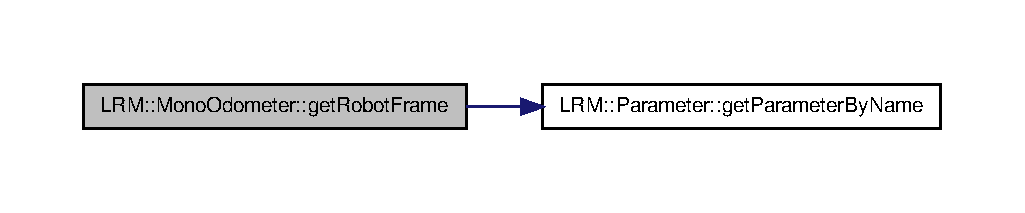
\includegraphics[width=350pt]{classLRM_1_1MonoOdometer_a3550a896dd2e212fa177d7401f1a5b61_cgraph}
\end{center}
\end{figure}


\hypertarget{classLRM_1_1MonoOdometer_a72b47de741d2c273a34c7d4e9a093092}{\index{\-L\-R\-M\-::\-Mono\-Odometer@{\-L\-R\-M\-::\-Mono\-Odometer}!get\-Sensor\-Frame@{get\-Sensor\-Frame}}
\index{get\-Sensor\-Frame@{get\-Sensor\-Frame}!LRM::MonoOdometer@{\-L\-R\-M\-::\-Mono\-Odometer}}
\subsubsection[{get\-Sensor\-Frame}]{\setlength{\rightskip}{0pt plus 5cm}std\-::string {\bf \-L\-R\-M\-::\-Mono\-Odometer\-::get\-Sensor\-Frame} (
\begin{DoxyParamCaption}
{}
\end{DoxyParamCaption}
)\hspace{0.3cm}{\ttfamily  \mbox{[}inline\mbox{]}}}}\label{classLRM_1_1MonoOdometer_a72b47de741d2c273a34c7d4e9a093092}


\-Here is the call graph for this function\-:\nopagebreak
\begin{figure}[H]
\begin{center}
\leavevmode
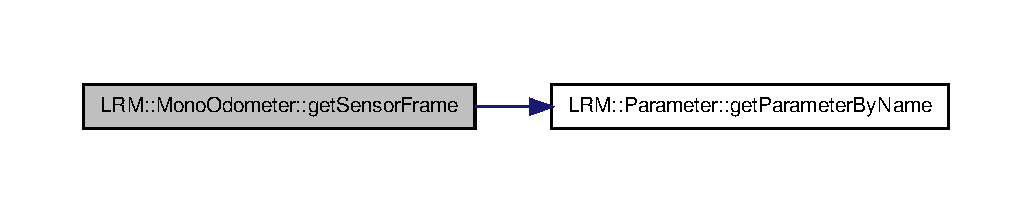
\includegraphics[width=350pt]{classLRM_1_1MonoOdometer_a72b47de741d2c273a34c7d4e9a093092_cgraph}
\end{center}
\end{figure}


\hypertarget{classLRM_1_1MonoOdometer_a7205e77893b1f9d4c37de616519ef5ed}{\index{\-L\-R\-M\-::\-Mono\-Odometer@{\-L\-R\-M\-::\-Mono\-Odometer}!\-Image\-Callback@{\-Image\-Callback}}
\index{\-Image\-Callback@{\-Image\-Callback}!LRM::MonoOdometer@{\-L\-R\-M\-::\-Mono\-Odometer}}
\subsubsection[{\-Image\-Callback}]{\setlength{\rightskip}{0pt plus 5cm}void {\bf \-L\-R\-M\-::\-Mono\-Odometer\-::\-Image\-Callback} (
\begin{DoxyParamCaption}
\item[{const sensor\-\_\-msgs\-::\-Image\-Const\-Ptr \&}]{msg}
\end{DoxyParamCaption}
)}}\label{classLRM_1_1MonoOdometer_a7205e77893b1f9d4c37de616519ef5ed}


\-The \-Image \-Callback method is responsible for handling the income messages from the camera device and extract the frame features and descriptors. 


\begin{DoxyParams}[1]{\-Parameters}
\mbox{\tt in}  & {\em msg} & \-Income message from the defined camera topic. \\
\hline
\end{DoxyParams}
\begin{DoxyRefDesc}{\-Todo}
\item[\hyperlink{todo__todo000001}{\-Todo}]\-What happens when it's not possible to estimate a motion? \-Kalman? \end{DoxyRefDesc}


\-Here is the call graph for this function\-:\nopagebreak
\begin{figure}[H]
\begin{center}
\leavevmode
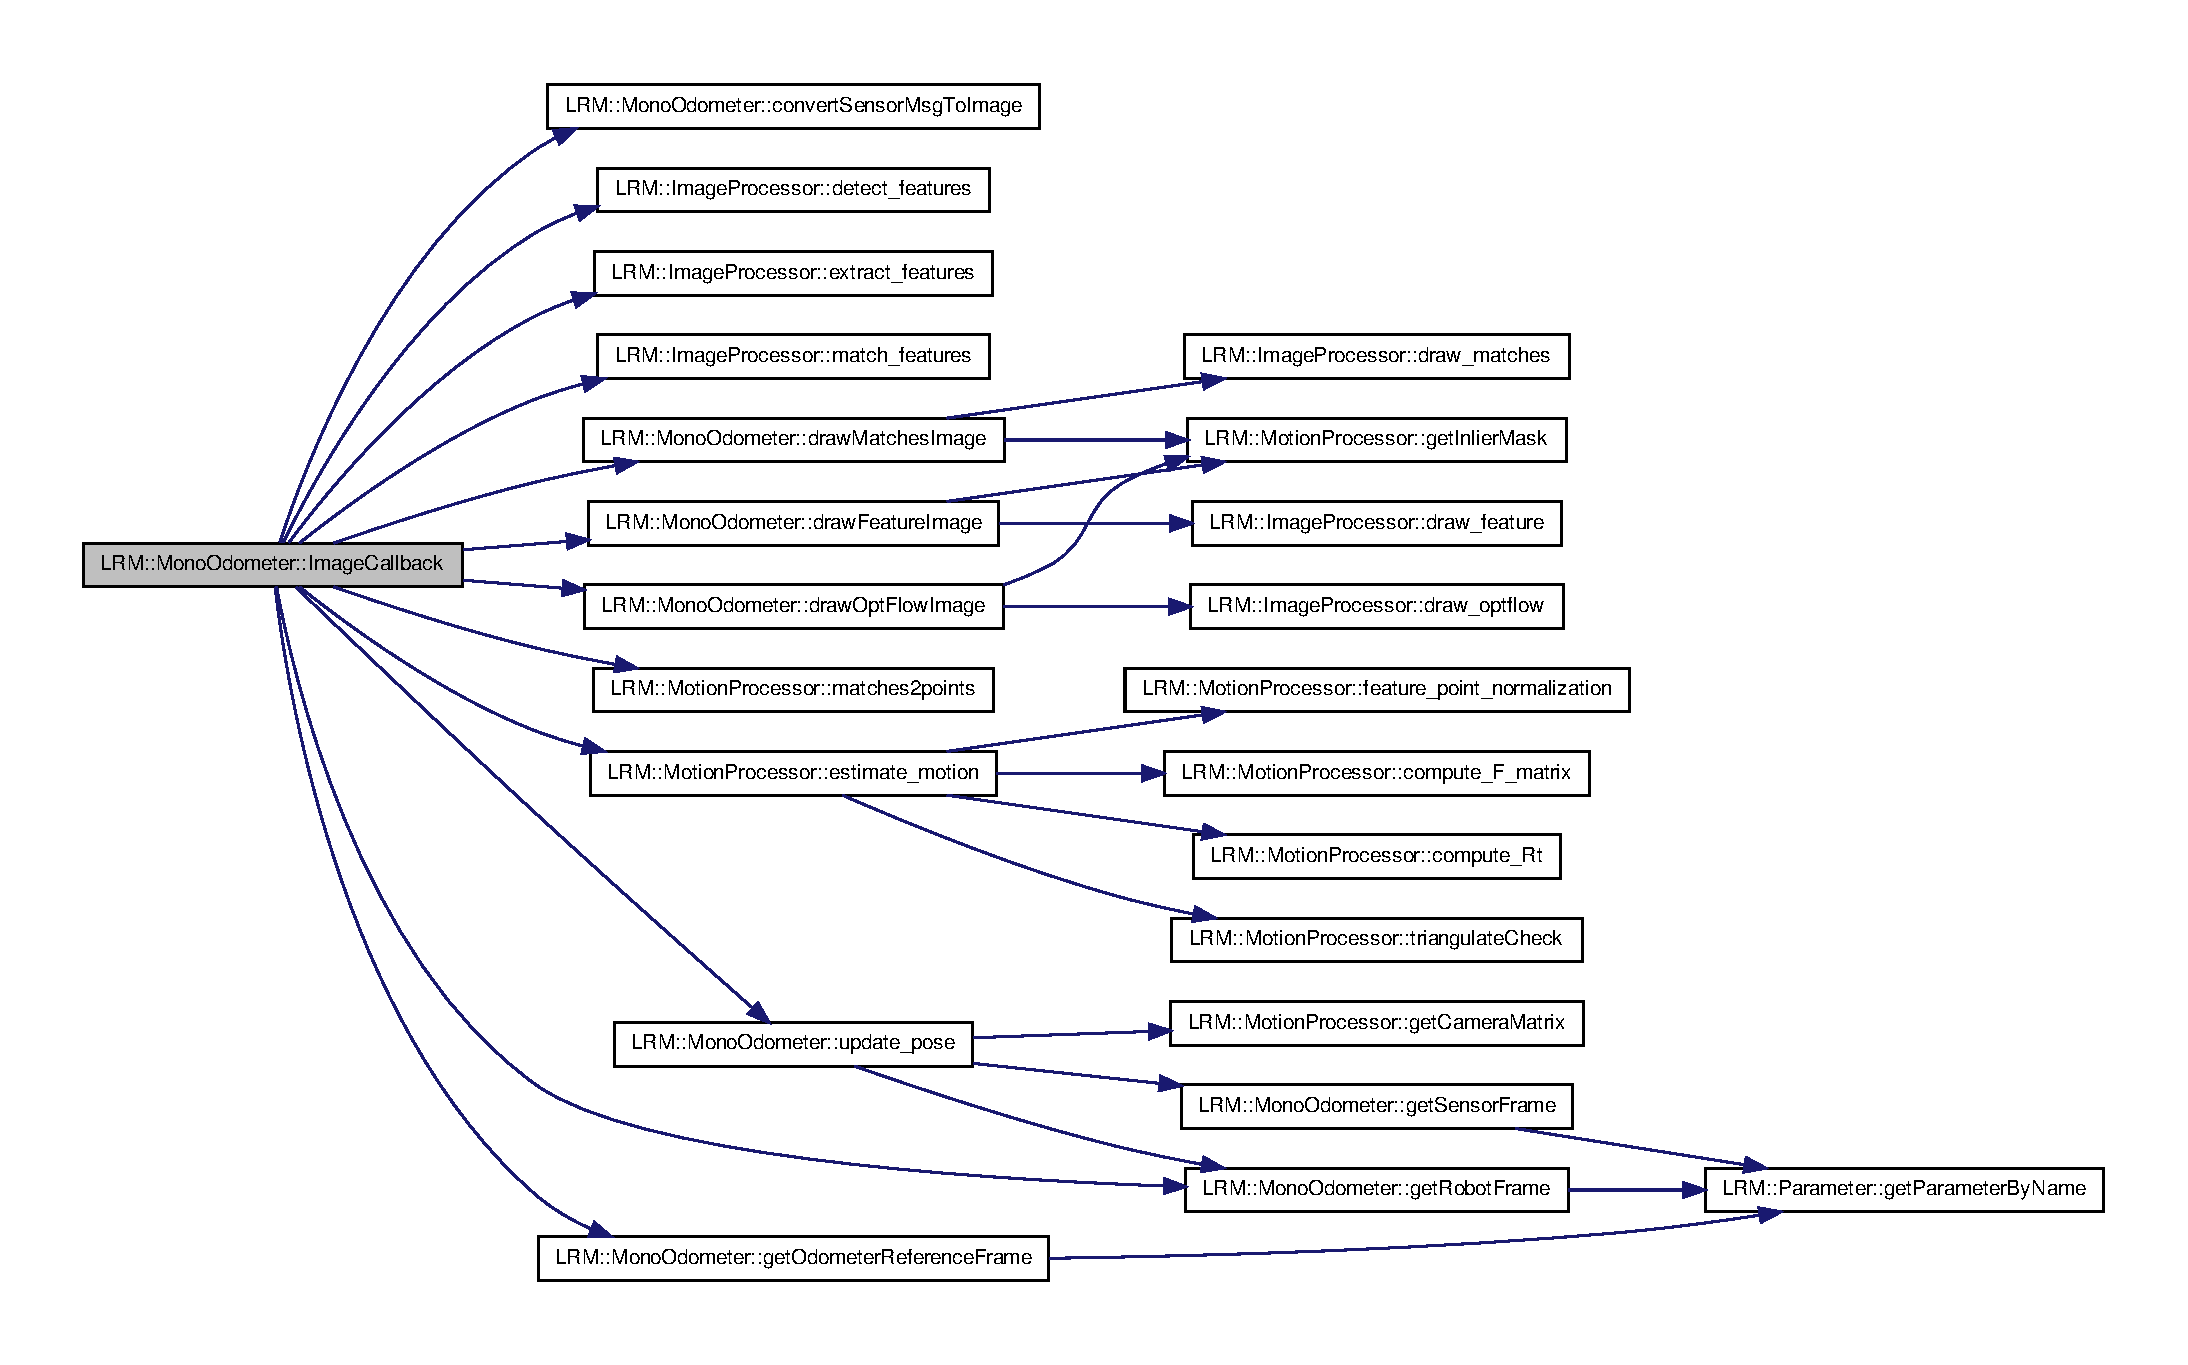
\includegraphics[width=350pt]{classLRM_1_1MonoOdometer_a7205e77893b1f9d4c37de616519ef5ed_cgraph}
\end{center}
\end{figure}


\hypertarget{classLRM_1_1MonoOdometer_aaea86d0c2fc1119b066b310451be4a67}{\index{\-L\-R\-M\-::\-Mono\-Odometer@{\-L\-R\-M\-::\-Mono\-Odometer}!is\-Intrinsic\-Matrix\-Path@{is\-Intrinsic\-Matrix\-Path}}
\index{is\-Intrinsic\-Matrix\-Path@{is\-Intrinsic\-Matrix\-Path}!LRM::MonoOdometer@{\-L\-R\-M\-::\-Mono\-Odometer}}
\subsubsection[{is\-Intrinsic\-Matrix\-Path}]{\setlength{\rightskip}{0pt plus 5cm}bool {\bf \-L\-R\-M\-::\-Mono\-Odometer\-::is\-Intrinsic\-Matrix\-Path} (
\begin{DoxyParamCaption}
{}
\end{DoxyParamCaption}
)\hspace{0.3cm}{\ttfamily  \mbox{[}inline\mbox{]}}}}\label{classLRM_1_1MonoOdometer_aaea86d0c2fc1119b066b310451be4a67}


\-Here is the call graph for this function\-:\nopagebreak
\begin{figure}[H]
\begin{center}
\leavevmode
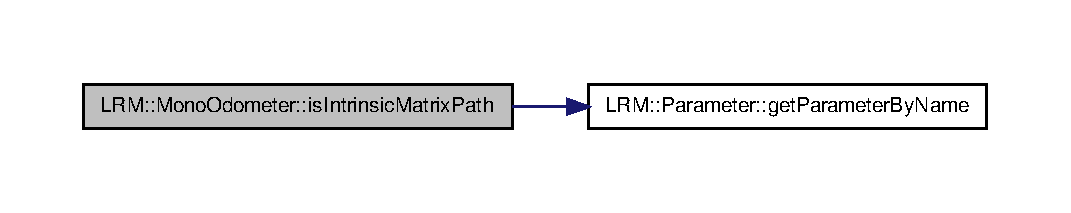
\includegraphics[width=350pt]{classLRM_1_1MonoOdometer_aaea86d0c2fc1119b066b310451be4a67_cgraph}
\end{center}
\end{figure}


\hypertarget{classLRM_1_1MonoOdometer_a8c7914efde9c07323c171d7adfaf656e}{\index{\-L\-R\-M\-::\-Mono\-Odometer@{\-L\-R\-M\-::\-Mono\-Odometer}!update\-\_\-pose@{update\-\_\-pose}}
\index{update\-\_\-pose@{update\-\_\-pose}!LRM::MonoOdometer@{\-L\-R\-M\-::\-Mono\-Odometer}}
\subsubsection[{update\-\_\-pose}]{\setlength{\rightskip}{0pt plus 5cm}int {\bf \-L\-R\-M\-::\-Mono\-Odometer\-::update\-\_\-pose} (
\begin{DoxyParamCaption}
{}
\end{DoxyParamCaption}
)\hspace{0.3cm}{\ttfamily  \mbox{[}private\mbox{]}}}}\label{classLRM_1_1MonoOdometer_a8c7914efde9c07323c171d7adfaf656e}


\-Here is the call graph for this function\-:\nopagebreak
\begin{figure}[H]
\begin{center}
\leavevmode
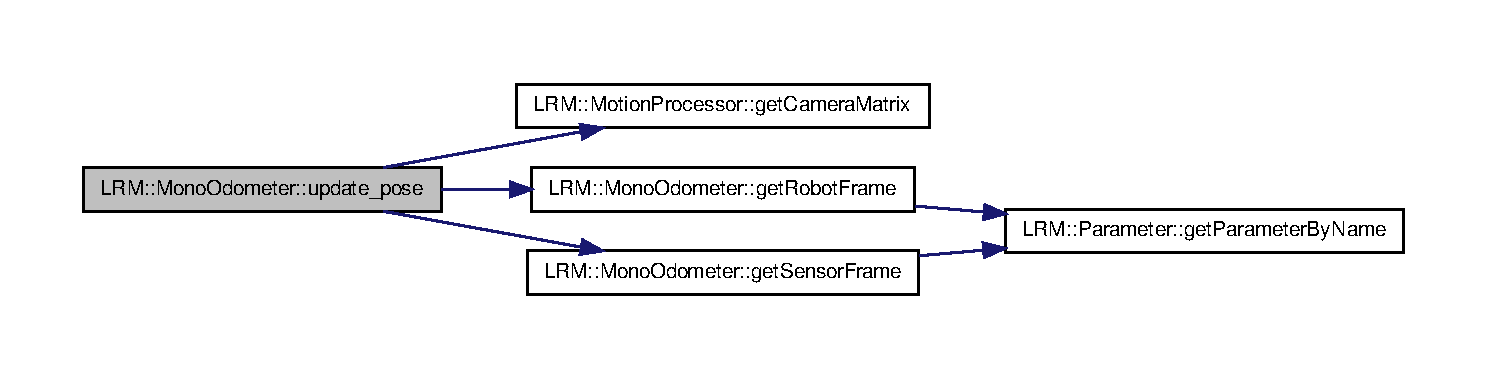
\includegraphics[width=350pt]{classLRM_1_1MonoOdometer_a8c7914efde9c07323c171d7adfaf656e_cgraph}
\end{center}
\end{figure}




\subsection{\-Member \-Data \-Documentation}
\hypertarget{classLRM_1_1MonoOdometer_a311831c9328491cde059e17706fd9bdc}{\index{\-L\-R\-M\-::\-Mono\-Odometer@{\-L\-R\-M\-::\-Mono\-Odometer}!base\-\_\-to\-\_\-sensor@{base\-\_\-to\-\_\-sensor}}
\index{base\-\_\-to\-\_\-sensor@{base\-\_\-to\-\_\-sensor}!LRM::MonoOdometer@{\-L\-R\-M\-::\-Mono\-Odometer}}
\subsubsection[{base\-\_\-to\-\_\-sensor}]{\setlength{\rightskip}{0pt plus 5cm}tf\-::\-Stamped\-Transform {\bf \-L\-R\-M\-::\-Mono\-Odometer\-::base\-\_\-to\-\_\-sensor}\hspace{0.3cm}{\ttfamily  \mbox{[}private\mbox{]}}}}\label{classLRM_1_1MonoOdometer_a311831c9328491cde059e17706fd9bdc}
\hypertarget{classLRM_1_1MonoOdometer_a166844b373399a94d688234592ae8468}{\index{\-L\-R\-M\-::\-Mono\-Odometer@{\-L\-R\-M\-::\-Mono\-Odometer}!feature\-\_\-image@{feature\-\_\-image}}
\index{feature\-\_\-image@{feature\-\_\-image}!LRM::MonoOdometer@{\-L\-R\-M\-::\-Mono\-Odometer}}
\subsubsection[{feature\-\_\-image}]{\setlength{\rightskip}{0pt plus 5cm}cv\-\_\-bridge\-::\-Cv\-Image {\bf \-L\-R\-M\-::\-Mono\-Odometer\-::feature\-\_\-image}\hspace{0.3cm}{\ttfamily  \mbox{[}private\mbox{]}}}}\label{classLRM_1_1MonoOdometer_a166844b373399a94d688234592ae8468}
\hypertarget{classLRM_1_1MonoOdometer_a49bef96a5413beea489f87dbb16eaf70}{\index{\-L\-R\-M\-::\-Mono\-Odometer@{\-L\-R\-M\-::\-Mono\-Odometer}!img\-\_\-proc@{img\-\_\-proc}}
\index{img\-\_\-proc@{img\-\_\-proc}!LRM::MonoOdometer@{\-L\-R\-M\-::\-Mono\-Odometer}}
\subsubsection[{img\-\_\-proc}]{\setlength{\rightskip}{0pt plus 5cm}{\bf \-Image\-Processor} {\bf \-L\-R\-M\-::\-Mono\-Odometer\-::img\-\_\-proc}\hspace{0.3cm}{\ttfamily  \mbox{[}private\mbox{]}}}}\label{classLRM_1_1MonoOdometer_a49bef96a5413beea489f87dbb16eaf70}
\hypertarget{classLRM_1_1MonoOdometer_a1bf24a1abdef05b79b54813058cad4a7}{\index{\-L\-R\-M\-::\-Mono\-Odometer@{\-L\-R\-M\-::\-Mono\-Odometer}!img\-\_\-proc\-\_\-parameter@{img\-\_\-proc\-\_\-parameter}}
\index{img\-\_\-proc\-\_\-parameter@{img\-\_\-proc\-\_\-parameter}!LRM::MonoOdometer@{\-L\-R\-M\-::\-Mono\-Odometer}}
\subsubsection[{img\-\_\-proc\-\_\-parameter}]{\setlength{\rightskip}{0pt plus 5cm}{\bf \-Image\-Processor\-Parameter} {\bf \-L\-R\-M\-::\-Mono\-Odometer\-::img\-\_\-proc\-\_\-parameter}\hspace{0.3cm}{\ttfamily  \mbox{[}private\mbox{]}}}}\label{classLRM_1_1MonoOdometer_a1bf24a1abdef05b79b54813058cad4a7}
\hypertarget{classLRM_1_1MonoOdometer_ad191c12993c8e8ee9200f71aec07057c}{\index{\-L\-R\-M\-::\-Mono\-Odometer@{\-L\-R\-M\-::\-Mono\-Odometer}!input\-\_\-image\-\_\-subscriber@{input\-\_\-image\-\_\-subscriber}}
\index{input\-\_\-image\-\_\-subscriber@{input\-\_\-image\-\_\-subscriber}!LRM::MonoOdometer@{\-L\-R\-M\-::\-Mono\-Odometer}}
\subsubsection[{input\-\_\-image\-\_\-subscriber}]{\setlength{\rightskip}{0pt plus 5cm}image\-\_\-transport\-::\-Subscriber {\bf \-L\-R\-M\-::\-Mono\-Odometer\-::input\-\_\-image\-\_\-subscriber}\hspace{0.3cm}{\ttfamily  \mbox{[}private\mbox{]}}}}\label{classLRM_1_1MonoOdometer_ad191c12993c8e8ee9200f71aec07057c}
\hypertarget{classLRM_1_1MonoOdometer_a7f874bb9b174d7a38085782377d5f195}{\index{\-L\-R\-M\-::\-Mono\-Odometer@{\-L\-R\-M\-::\-Mono\-Odometer}!\-K@{\-K}}
\index{\-K@{\-K}!LRM::MonoOdometer@{\-L\-R\-M\-::\-Mono\-Odometer}}
\subsubsection[{\-K}]{\setlength{\rightskip}{0pt plus 5cm}cv\-::\-Mat {\bf \-L\-R\-M\-::\-Mono\-Odometer\-::\-K}\hspace{0.3cm}{\ttfamily  \mbox{[}private\mbox{]}}}}\label{classLRM_1_1MonoOdometer_a7f874bb9b174d7a38085782377d5f195}
\hypertarget{classLRM_1_1MonoOdometer_aefc5720615c86208707622253d2e08ed}{\index{\-L\-R\-M\-::\-Mono\-Odometer@{\-L\-R\-M\-::\-Mono\-Odometer}!matches@{matches}}
\index{matches@{matches}!LRM::MonoOdometer@{\-L\-R\-M\-::\-Mono\-Odometer}}
\subsubsection[{matches}]{\setlength{\rightskip}{0pt plus 5cm}std\-::vector$<$cv\-::\-D\-Match$>$ {\bf \-L\-R\-M\-::\-Mono\-Odometer\-::matches}\hspace{0.3cm}{\ttfamily  \mbox{[}private\mbox{]}}}}\label{classLRM_1_1MonoOdometer_aefc5720615c86208707622253d2e08ed}
\hypertarget{classLRM_1_1MonoOdometer_a1646743b51e5e0386def055e0265aaf2}{\index{\-L\-R\-M\-::\-Mono\-Odometer@{\-L\-R\-M\-::\-Mono\-Odometer}!matches\-\_\-image@{matches\-\_\-image}}
\index{matches\-\_\-image@{matches\-\_\-image}!LRM::MonoOdometer@{\-L\-R\-M\-::\-Mono\-Odometer}}
\subsubsection[{matches\-\_\-image}]{\setlength{\rightskip}{0pt plus 5cm}cv\-\_\-bridge\-::\-Cv\-Image {\bf \-L\-R\-M\-::\-Mono\-Odometer\-::matches\-\_\-image}\hspace{0.3cm}{\ttfamily  \mbox{[}private\mbox{]}}}}\label{classLRM_1_1MonoOdometer_a1646743b51e5e0386def055e0265aaf2}
\hypertarget{classLRM_1_1MonoOdometer_a91b2fd9ac3051a11e7008c2e3740a382}{\index{\-L\-R\-M\-::\-Mono\-Odometer@{\-L\-R\-M\-::\-Mono\-Odometer}!mot\-\_\-proc@{mot\-\_\-proc}}
\index{mot\-\_\-proc@{mot\-\_\-proc}!LRM::MonoOdometer@{\-L\-R\-M\-::\-Mono\-Odometer}}
\subsubsection[{mot\-\_\-proc}]{\setlength{\rightskip}{0pt plus 5cm}{\bf \-Motion\-Processor} {\bf \-L\-R\-M\-::\-Mono\-Odometer\-::mot\-\_\-proc}\hspace{0.3cm}{\ttfamily  \mbox{[}private\mbox{]}}}}\label{classLRM_1_1MonoOdometer_a91b2fd9ac3051a11e7008c2e3740a382}
\hypertarget{classLRM_1_1MonoOdometer_a8bf0ca69100b032fe3c73fb1e0bed318}{\index{\-L\-R\-M\-::\-Mono\-Odometer@{\-L\-R\-M\-::\-Mono\-Odometer}!mot\-\_\-proc\-\_\-parameter@{mot\-\_\-proc\-\_\-parameter}}
\index{mot\-\_\-proc\-\_\-parameter@{mot\-\_\-proc\-\_\-parameter}!LRM::MonoOdometer@{\-L\-R\-M\-::\-Mono\-Odometer}}
\subsubsection[{mot\-\_\-proc\-\_\-parameter}]{\setlength{\rightskip}{0pt plus 5cm}{\bf \-Motion\-Processor\-Parameter} {\bf \-L\-R\-M\-::\-Mono\-Odometer\-::mot\-\_\-proc\-\_\-parameter}\hspace{0.3cm}{\ttfamily  \mbox{[}private\mbox{]}}}}\label{classLRM_1_1MonoOdometer_a8bf0ca69100b032fe3c73fb1e0bed318}
\hypertarget{classLRM_1_1MonoOdometer_a85bf06a46a0367a821f145e1c3f51e8c}{\index{\-L\-R\-M\-::\-Mono\-Odometer@{\-L\-R\-M\-::\-Mono\-Odometer}!odom\-\_\-broadcaster@{odom\-\_\-broadcaster}}
\index{odom\-\_\-broadcaster@{odom\-\_\-broadcaster}!LRM::MonoOdometer@{\-L\-R\-M\-::\-Mono\-Odometer}}
\subsubsection[{odom\-\_\-broadcaster}]{\setlength{\rightskip}{0pt plus 5cm}tf\-::\-Transform\-Broadcaster {\bf \-L\-R\-M\-::\-Mono\-Odometer\-::odom\-\_\-broadcaster}\hspace{0.3cm}{\ttfamily  \mbox{[}private\mbox{]}}}}\label{classLRM_1_1MonoOdometer_a85bf06a46a0367a821f145e1c3f51e8c}
\hypertarget{classLRM_1_1MonoOdometer_afdc33ed78a3234b3469e094b23b4d511}{\index{\-L\-R\-M\-::\-Mono\-Odometer@{\-L\-R\-M\-::\-Mono\-Odometer}!odometry@{odometry}}
\index{odometry@{odometry}!LRM::MonoOdometer@{\-L\-R\-M\-::\-Mono\-Odometer}}
\subsubsection[{odometry}]{\setlength{\rightskip}{0pt plus 5cm}nav\-\_\-msgs\-::\-Odometry {\bf \-L\-R\-M\-::\-Mono\-Odometer\-::odometry}\hspace{0.3cm}{\ttfamily  \mbox{[}private\mbox{]}}}}\label{classLRM_1_1MonoOdometer_afdc33ed78a3234b3469e094b23b4d511}
\hypertarget{classLRM_1_1MonoOdometer_a113a9a4905bb7c9f19df55610802ffec}{\index{\-L\-R\-M\-::\-Mono\-Odometer@{\-L\-R\-M\-::\-Mono\-Odometer}!odometry\-\_\-advertiser@{odometry\-\_\-advertiser}}
\index{odometry\-\_\-advertiser@{odometry\-\_\-advertiser}!LRM::MonoOdometer@{\-L\-R\-M\-::\-Mono\-Odometer}}
\subsubsection[{odometry\-\_\-advertiser}]{\setlength{\rightskip}{0pt plus 5cm}ros\-::\-Publisher {\bf \-L\-R\-M\-::\-Mono\-Odometer\-::odometry\-\_\-advertiser}\hspace{0.3cm}{\ttfamily  \mbox{[}private\mbox{]}}}}\label{classLRM_1_1MonoOdometer_a113a9a4905bb7c9f19df55610802ffec}
\hypertarget{classLRM_1_1MonoOdometer_a5f9b4ef57cf2b7d88bb92c8269a8792d}{\index{\-L\-R\-M\-::\-Mono\-Odometer@{\-L\-R\-M\-::\-Mono\-Odometer}!optflow\-\_\-image@{optflow\-\_\-image}}
\index{optflow\-\_\-image@{optflow\-\_\-image}!LRM::MonoOdometer@{\-L\-R\-M\-::\-Mono\-Odometer}}
\subsubsection[{optflow\-\_\-image}]{\setlength{\rightskip}{0pt plus 5cm}cv\-\_\-bridge\-::\-Cv\-Image {\bf \-L\-R\-M\-::\-Mono\-Odometer\-::optflow\-\_\-image}\hspace{0.3cm}{\ttfamily  \mbox{[}private\mbox{]}}}}\label{classLRM_1_1MonoOdometer_a5f9b4ef57cf2b7d88bb92c8269a8792d}
\hypertarget{classLRM_1_1MonoOdometer_abcc8b0e66d3629d66b74e8d857adea9e}{\index{\-L\-R\-M\-::\-Mono\-Odometer@{\-L\-R\-M\-::\-Mono\-Odometer}!output\-\_\-feature\-\_\-advertiser@{output\-\_\-feature\-\_\-advertiser}}
\index{output\-\_\-feature\-\_\-advertiser@{output\-\_\-feature\-\_\-advertiser}!LRM::MonoOdometer@{\-L\-R\-M\-::\-Mono\-Odometer}}
\subsubsection[{output\-\_\-feature\-\_\-advertiser}]{\setlength{\rightskip}{0pt plus 5cm}image\-\_\-transport\-::\-Publisher {\bf \-L\-R\-M\-::\-Mono\-Odometer\-::output\-\_\-feature\-\_\-advertiser}\hspace{0.3cm}{\ttfamily  \mbox{[}private\mbox{]}}}}\label{classLRM_1_1MonoOdometer_abcc8b0e66d3629d66b74e8d857adea9e}
\hypertarget{classLRM_1_1MonoOdometer_ab3e372106292ea873dc5428e1b3d0026}{\index{\-L\-R\-M\-::\-Mono\-Odometer@{\-L\-R\-M\-::\-Mono\-Odometer}!output\-\_\-matches\-\_\-advertiser@{output\-\_\-matches\-\_\-advertiser}}
\index{output\-\_\-matches\-\_\-advertiser@{output\-\_\-matches\-\_\-advertiser}!LRM::MonoOdometer@{\-L\-R\-M\-::\-Mono\-Odometer}}
\subsubsection[{output\-\_\-matches\-\_\-advertiser}]{\setlength{\rightskip}{0pt plus 5cm}image\-\_\-transport\-::\-Publisher {\bf \-L\-R\-M\-::\-Mono\-Odometer\-::output\-\_\-matches\-\_\-advertiser}\hspace{0.3cm}{\ttfamily  \mbox{[}private\mbox{]}}}}\label{classLRM_1_1MonoOdometer_ab3e372106292ea873dc5428e1b3d0026}
\hypertarget{classLRM_1_1MonoOdometer_a2f9dcb6ceed7b4b85e0df512fc297105}{\index{\-L\-R\-M\-::\-Mono\-Odometer@{\-L\-R\-M\-::\-Mono\-Odometer}!output\-\_\-optflow\-\_\-advertiser@{output\-\_\-optflow\-\_\-advertiser}}
\index{output\-\_\-optflow\-\_\-advertiser@{output\-\_\-optflow\-\_\-advertiser}!LRM::MonoOdometer@{\-L\-R\-M\-::\-Mono\-Odometer}}
\subsubsection[{output\-\_\-optflow\-\_\-advertiser}]{\setlength{\rightskip}{0pt plus 5cm}image\-\_\-transport\-::\-Publisher {\bf \-L\-R\-M\-::\-Mono\-Odometer\-::output\-\_\-optflow\-\_\-advertiser}\hspace{0.3cm}{\ttfamily  \mbox{[}private\mbox{]}}}}\label{classLRM_1_1MonoOdometer_a2f9dcb6ceed7b4b85e0df512fc297105}
\hypertarget{classLRM_1_1MonoOdometer_a086c208e839df4586e99d417c60a3d77}{\index{\-L\-R\-M\-::\-Mono\-Odometer@{\-L\-R\-M\-::\-Mono\-Odometer}!pose@{pose}}
\index{pose@{pose}!LRM::MonoOdometer@{\-L\-R\-M\-::\-Mono\-Odometer}}
\subsubsection[{pose}]{\setlength{\rightskip}{0pt plus 5cm}tf\-::\-Transform {\bf \-L\-R\-M\-::\-Mono\-Odometer\-::pose}\hspace{0.3cm}{\ttfamily  \mbox{[}private\mbox{]}}}}\label{classLRM_1_1MonoOdometer_a086c208e839df4586e99d417c60a3d77}
\hypertarget{classLRM_1_1MonoOdometer_a7bf26df30d6cebf7e6c5b85c2318ff51}{\index{\-L\-R\-M\-::\-Mono\-Odometer@{\-L\-R\-M\-::\-Mono\-Odometer}!query\-\_\-desc@{query\-\_\-desc}}
\index{query\-\_\-desc@{query\-\_\-desc}!LRM::MonoOdometer@{\-L\-R\-M\-::\-Mono\-Odometer}}
\subsubsection[{query\-\_\-desc}]{\setlength{\rightskip}{0pt plus 5cm}cv\-::\-Mat {\bf \-L\-R\-M\-::\-Mono\-Odometer\-::query\-\_\-desc}\hspace{0.3cm}{\ttfamily  \mbox{[}private\mbox{]}}}}\label{classLRM_1_1MonoOdometer_a7bf26df30d6cebf7e6c5b85c2318ff51}
\hypertarget{classLRM_1_1MonoOdometer_a1fbec0b090c10b1c542bd86f18795a14}{\index{\-L\-R\-M\-::\-Mono\-Odometer@{\-L\-R\-M\-::\-Mono\-Odometer}!query\-\_\-image@{query\-\_\-image}}
\index{query\-\_\-image@{query\-\_\-image}!LRM::MonoOdometer@{\-L\-R\-M\-::\-Mono\-Odometer}}
\subsubsection[{query\-\_\-image}]{\setlength{\rightskip}{0pt plus 5cm}cv\-\_\-bridge\-::\-Cv\-Image\-Const\-Ptr {\bf \-L\-R\-M\-::\-Mono\-Odometer\-::query\-\_\-image}\hspace{0.3cm}{\ttfamily  \mbox{[}private\mbox{]}}}}\label{classLRM_1_1MonoOdometer_a1fbec0b090c10b1c542bd86f18795a14}


\-Current image. 

\hypertarget{classLRM_1_1MonoOdometer_a18d64f992353bf50e1421a1cb9ca32f2}{\index{\-L\-R\-M\-::\-Mono\-Odometer@{\-L\-R\-M\-::\-Mono\-Odometer}!query\-\_\-kpts@{query\-\_\-kpts}}
\index{query\-\_\-kpts@{query\-\_\-kpts}!LRM::MonoOdometer@{\-L\-R\-M\-::\-Mono\-Odometer}}
\subsubsection[{query\-\_\-kpts}]{\setlength{\rightskip}{0pt plus 5cm}std\-::vector$<$cv\-::\-Key\-Point$>$ {\bf \-L\-R\-M\-::\-Mono\-Odometer\-::query\-\_\-kpts}\hspace{0.3cm}{\ttfamily  \mbox{[}private\mbox{]}}}}\label{classLRM_1_1MonoOdometer_a18d64f992353bf50e1421a1cb9ca32f2}


\-Current image keypoints. 

\hypertarget{classLRM_1_1MonoOdometer_a4d269a8b3827580e73515e8f958e2283}{\index{\-L\-R\-M\-::\-Mono\-Odometer@{\-L\-R\-M\-::\-Mono\-Odometer}!query\-\_\-pts@{query\-\_\-pts}}
\index{query\-\_\-pts@{query\-\_\-pts}!LRM::MonoOdometer@{\-L\-R\-M\-::\-Mono\-Odometer}}
\subsubsection[{query\-\_\-pts}]{\setlength{\rightskip}{0pt plus 5cm}std\-::vector$<$cv\-::\-Point2d$>$ {\bf \-L\-R\-M\-::\-Mono\-Odometer\-::query\-\_\-pts}\hspace{0.3cm}{\ttfamily  \mbox{[}private\mbox{]}}}}\label{classLRM_1_1MonoOdometer_a4d269a8b3827580e73515e8f958e2283}
\hypertarget{classLRM_1_1MonoOdometer_ae201ba1988badf708c046e1b29b70ab1}{\index{\-L\-R\-M\-::\-Mono\-Odometer@{\-L\-R\-M\-::\-Mono\-Odometer}!query\-\_\-timestamp@{query\-\_\-timestamp}}
\index{query\-\_\-timestamp@{query\-\_\-timestamp}!LRM::MonoOdometer@{\-L\-R\-M\-::\-Mono\-Odometer}}
\subsubsection[{query\-\_\-timestamp}]{\setlength{\rightskip}{0pt plus 5cm}ros\-::\-Time {\bf \-L\-R\-M\-::\-Mono\-Odometer\-::query\-\_\-timestamp}\hspace{0.3cm}{\ttfamily  \mbox{[}private\mbox{]}}}}\label{classLRM_1_1MonoOdometer_ae201ba1988badf708c046e1b29b70ab1}
\hypertarget{classLRM_1_1MonoOdometer_a7667abb4e8d035e25811c63e6af42ae3}{\index{\-L\-R\-M\-::\-Mono\-Odometer@{\-L\-R\-M\-::\-Mono\-Odometer}!ros\-\_\-parameter@{ros\-\_\-parameter}}
\index{ros\-\_\-parameter@{ros\-\_\-parameter}!LRM::MonoOdometer@{\-L\-R\-M\-::\-Mono\-Odometer}}
\subsubsection[{ros\-\_\-parameter}]{\setlength{\rightskip}{0pt plus 5cm}{\bf \-R\-O\-S\-Parameter} {\bf \-L\-R\-M\-::\-Mono\-Odometer\-::ros\-\_\-parameter}\hspace{0.3cm}{\ttfamily  \mbox{[}private\mbox{]}}}}\label{classLRM_1_1MonoOdometer_a7667abb4e8d035e25811c63e6af42ae3}
\hypertarget{classLRM_1_1MonoOdometer_aa17423bfec7b2a995672d40cc6ed4fbe}{\index{\-L\-R\-M\-::\-Mono\-Odometer@{\-L\-R\-M\-::\-Mono\-Odometer}!tf\-\_\-listener@{tf\-\_\-listener}}
\index{tf\-\_\-listener@{tf\-\_\-listener}!LRM::MonoOdometer@{\-L\-R\-M\-::\-Mono\-Odometer}}
\subsubsection[{tf\-\_\-listener}]{\setlength{\rightskip}{0pt plus 5cm}tf\-::\-Transform\-Listener {\bf \-L\-R\-M\-::\-Mono\-Odometer\-::tf\-\_\-listener}\hspace{0.3cm}{\ttfamily  \mbox{[}private\mbox{]}}}}\label{classLRM_1_1MonoOdometer_aa17423bfec7b2a995672d40cc6ed4fbe}
\hypertarget{classLRM_1_1MonoOdometer_aae6c2096b1b0c785548bc57cf6557427}{\index{\-L\-R\-M\-::\-Mono\-Odometer@{\-L\-R\-M\-::\-Mono\-Odometer}!train\-\_\-desc@{train\-\_\-desc}}
\index{train\-\_\-desc@{train\-\_\-desc}!LRM::MonoOdometer@{\-L\-R\-M\-::\-Mono\-Odometer}}
\subsubsection[{train\-\_\-desc}]{\setlength{\rightskip}{0pt plus 5cm}cv\-::\-Mat {\bf \-L\-R\-M\-::\-Mono\-Odometer\-::train\-\_\-desc}\hspace{0.3cm}{\ttfamily  \mbox{[}private\mbox{]}}}}\label{classLRM_1_1MonoOdometer_aae6c2096b1b0c785548bc57cf6557427}
\hypertarget{classLRM_1_1MonoOdometer_a91ee6e52006559ba0f769a2ccc06fa64}{\index{\-L\-R\-M\-::\-Mono\-Odometer@{\-L\-R\-M\-::\-Mono\-Odometer}!train\-\_\-image@{train\-\_\-image}}
\index{train\-\_\-image@{train\-\_\-image}!LRM::MonoOdometer@{\-L\-R\-M\-::\-Mono\-Odometer}}
\subsubsection[{train\-\_\-image}]{\setlength{\rightskip}{0pt plus 5cm}cv\-\_\-bridge\-::\-Cv\-Image\-Const\-Ptr {\bf \-L\-R\-M\-::\-Mono\-Odometer\-::train\-\_\-image}\hspace{0.3cm}{\ttfamily  \mbox{[}private\mbox{]}}}}\label{classLRM_1_1MonoOdometer_a91ee6e52006559ba0f769a2ccc06fa64}


\-Previous image. 

\hypertarget{classLRM_1_1MonoOdometer_a98515916ee97beaefb9bbcf07cd02d1b}{\index{\-L\-R\-M\-::\-Mono\-Odometer@{\-L\-R\-M\-::\-Mono\-Odometer}!train\-\_\-kpts@{train\-\_\-kpts}}
\index{train\-\_\-kpts@{train\-\_\-kpts}!LRM::MonoOdometer@{\-L\-R\-M\-::\-Mono\-Odometer}}
\subsubsection[{train\-\_\-kpts}]{\setlength{\rightskip}{0pt plus 5cm}std\-::vector$<$cv\-::\-Key\-Point$>$ {\bf \-L\-R\-M\-::\-Mono\-Odometer\-::train\-\_\-kpts}\hspace{0.3cm}{\ttfamily  \mbox{[}private\mbox{]}}}}\label{classLRM_1_1MonoOdometer_a98515916ee97beaefb9bbcf07cd02d1b}


\-Previous image keypoints. 

\hypertarget{classLRM_1_1MonoOdometer_accbdc3f32cf2fb8e75f3f40cd8a4e60e}{\index{\-L\-R\-M\-::\-Mono\-Odometer@{\-L\-R\-M\-::\-Mono\-Odometer}!train\-\_\-pts@{train\-\_\-pts}}
\index{train\-\_\-pts@{train\-\_\-pts}!LRM::MonoOdometer@{\-L\-R\-M\-::\-Mono\-Odometer}}
\subsubsection[{train\-\_\-pts}]{\setlength{\rightskip}{0pt plus 5cm}std\-::vector$<$cv\-::\-Point2d$>$ {\bf \-L\-R\-M\-::\-Mono\-Odometer\-::train\-\_\-pts}\hspace{0.3cm}{\ttfamily  \mbox{[}private\mbox{]}}}}\label{classLRM_1_1MonoOdometer_accbdc3f32cf2fb8e75f3f40cd8a4e60e}
\hypertarget{classLRM_1_1MonoOdometer_a7024b12b516c41771d59046471ea7319}{\index{\-L\-R\-M\-::\-Mono\-Odometer@{\-L\-R\-M\-::\-Mono\-Odometer}!train\-\_\-timestamp@{train\-\_\-timestamp}}
\index{train\-\_\-timestamp@{train\-\_\-timestamp}!LRM::MonoOdometer@{\-L\-R\-M\-::\-Mono\-Odometer}}
\subsubsection[{train\-\_\-timestamp}]{\setlength{\rightskip}{0pt plus 5cm}ros\-::\-Time {\bf \-L\-R\-M\-::\-Mono\-Odometer\-::train\-\_\-timestamp}\hspace{0.3cm}{\ttfamily  \mbox{[}private\mbox{]}}}}\label{classLRM_1_1MonoOdometer_a7024b12b516c41771d59046471ea7319}


\-The documentation for this class was generated from the following files\-:\begin{DoxyCompactItemize}
\item 
include/\hyperlink{mono__odometer_8h}{mono\-\_\-odometer.\-h}\item 
src/\hyperlink{mono__odometer_8cpp}{mono\-\_\-odometer.\-cpp}\end{DoxyCompactItemize}

\hypertarget{classLRM_1_1MotionProcessor}{\section{\-L\-R\-M\-:\-:\-Motion\-Processor \-Class \-Reference}
\label{classLRM_1_1MotionProcessor}\index{\-L\-R\-M\-::\-Motion\-Processor@{\-L\-R\-M\-::\-Motion\-Processor}}
}


{\ttfamily \#include $<$motion\-\_\-processor.\-h$>$}

\subsection*{\-Public \-Member \-Functions}
\begin{DoxyCompactItemize}
\item 
\hyperlink{classLRM_1_1MotionProcessor_a76c8a7c000e36f3cb5c5f44b10440a85}{\-Motion\-Processor} ()
\item 
virtual \hyperlink{classLRM_1_1MotionProcessor_a465b73032fda5b158e0b0dc8f48080ff}{$\sim$\-Motion\-Processor} ()
\item 
int \hyperlink{classLRM_1_1MotionProcessor_a64c33eeeac78f7f8358c77daa4635689}{setting} (\hyperlink{classLRM_1_1MotionProcessorParameter}{\-Motion\-Processor\-Parameter} param)
\item 
void \hyperlink{classLRM_1_1MotionProcessor_a2fa4b7f533a12a88058a63b87ad96f4a}{matches2points} (const std\-::vector$<$ cv\-::\-Key\-Point $>$ \&query, const std\-::vector$<$ cv\-::\-Key\-Point $>$ \&train, const std\-::vector$<$ cv\-::\-D\-Match $>$ \&matches, std\-::vector$<$ cv\-::\-Point2d $>$ \&\hyperlink{classLRM_1_1MotionProcessor_af0e2f9ee5479177b49a6caf44962faff}{query\-\_\-pts}, std\-::vector$<$ cv\-::\-Point2d $>$ \&\hyperlink{classLRM_1_1MotionProcessor_ae72b3aea2c352caefb7f256a40ca6e31}{train\-\_\-pts})
\item 
void \hyperlink{classLRM_1_1MotionProcessor_a13ac0902eb981cacc1dee1a2d586362d}{estimate\-\_\-motion} (std\-::vector$<$ cv\-::\-Point2d $>$ \hyperlink{classLRM_1_1MotionProcessor_ae72b3aea2c352caefb7f256a40ca6e31}{train\-\_\-pts}, std\-::vector$<$ cv\-::\-Point2d $>$ \hyperlink{classLRM_1_1MotionProcessor_af0e2f9ee5479177b49a6caf44962faff}{query\-\_\-pts}, std\-::vector$<$ cv\-::\-D\-Match $>$ matches, cv\-::\-Mat \-K)
\begin{DoxyCompactList}\small\item\em \-Estimates the rotation and translation between two frames. \end{DoxyCompactList}\item 
bool \hyperlink{classLRM_1_1MotionProcessor_aa5cf91a28041e8897469a9ba9bd4b35b}{feature\-\_\-point\-\_\-normalization} (std\-::vector$<$ cv\-::\-Point2d $>$ \hyperlink{classLRM_1_1MotionProcessor_af0e2f9ee5479177b49a6caf44962faff}{query\-\_\-pts}, std\-::vector$<$ cv\-::\-Point2d $>$ \hyperlink{classLRM_1_1MotionProcessor_ae72b3aea2c352caefb7f256a40ca6e31}{train\-\_\-pts}, std\-::vector$<$ cv\-::\-Point2d $>$ \&norm\-\_\-query\-\_\-pts, std\-::vector$<$ cv\-::\-Point2d $>$ \&norm\-\_\-train\-\_\-pts, cv\-::\-Mat \&\-Tc, cv\-::\-Mat \&\-Tp)
\item 
cv\-::\-Mat \hyperlink{classLRM_1_1MotionProcessor_aa06b8d787d57f51f99a0281582a136bc}{compute\-\_\-\-F\-\_\-matrix} (std\-::vector$<$ cv\-::\-Point2d $>$ \hyperlink{classLRM_1_1MotionProcessor_ae72b3aea2c352caefb7f256a40ca6e31}{train\-\_\-pts}, std\-::vector$<$ cv\-::\-Point2d $>$ \hyperlink{classLRM_1_1MotionProcessor_af0e2f9ee5479177b49a6caf44962faff}{query\-\_\-pts})
\item 
std\-::vector$<$ cv\-::\-Mat $>$ \hyperlink{classLRM_1_1MotionProcessor_af5cedadc3cafc249f88012884909b138}{compute\-\_\-\-Rt} (cv\-::\-Mat \-E, cv\-::\-Mat \-K)
\item 
int \hyperlink{classLRM_1_1MotionProcessor_a14ef29f158bf0fe19d05dbadc81e64a0}{triangulate\-Check} (std\-::vector$<$ cv\-::\-Point2d $>$ \hyperlink{classLRM_1_1MotionProcessor_ae72b3aea2c352caefb7f256a40ca6e31}{train\-\_\-pts}, std\-::vector$<$ cv\-::\-Point2d $>$ \hyperlink{classLRM_1_1MotionProcessor_af0e2f9ee5479177b49a6caf44962faff}{query\-\_\-pts}, cv\-::\-Mat \&\-K, cv\-::\-Mat \hyperlink{classLRM_1_1MotionProcessor_a84d9c7cce3207b43bb79988c32d07f23}{\-P}, std\-::vector$<$ char $>$ mask=std\-::vector$<$ char $>$())
\item 
int \hyperlink{classLRM_1_1MotionProcessor_a6d556c3dd5d0c682c407e65b51e2207e}{cheirality\-Check} (cv\-::\-Mat \-P2, cv\-::\-Mat \-K, std\-::vector$<$ cv\-::\-Point2d $>$ pp, std\-::vector$<$ cv\-::\-Point2d $>$ pc)
\item 
cv\-::\-Mat \hyperlink{classLRM_1_1MotionProcessor_a848e86c9fc94cf58de7c4f6ae7e50267}{\-Rodrigues} (cv\-::\-Vec3d omega, double theta=-\/1)
\item 
double \hyperlink{classLRM_1_1MotionProcessor_ac0000e0136ca3c117f1fc548b72d9912}{triple\-\_\-product} (cv\-::\-Vec3d a, cv\-::\-Vec3d b, cv\-::\-Vec3d c)
\item 
cv\-::\-Mat \hyperlink{classLRM_1_1MotionProcessor_a3254a463388e2a6db96e81aa29f5b72e}{skew} (cv\-::\-Vec3d a)
\item 
std\-::vector$<$ char $>$ \hyperlink{classLRM_1_1MotionProcessor_afea20e7bd776f189fabdd259c22e6b4e}{get\-Inlier\-Mask} ()
\item 
cv\-::\-Mat \hyperlink{classLRM_1_1MotionProcessor_a8029258b4e6d79233b7340eb7695b4f0}{get\-Camera\-Matrix} ()
\end{DoxyCompactItemize}
\subsection*{\-Private \-Attributes}
\begin{DoxyCompactItemize}
\item 
std\-::vector$<$ char $>$ \hyperlink{classLRM_1_1MotionProcessor_a1cebe392055fdfe8002def6c7810f754}{inliers}
\item 
std\-::vector$<$ cv\-::\-Point2d $>$ \hyperlink{classLRM_1_1MotionProcessor_ae72b3aea2c352caefb7f256a40ca6e31}{train\-\_\-pts}
\item 
std\-::vector$<$ cv\-::\-Point2d $>$ \hyperlink{classLRM_1_1MotionProcessor_af0e2f9ee5479177b49a6caf44962faff}{query\-\_\-pts}
\item 
cv\-::\-Mat \hyperlink{classLRM_1_1MotionProcessor_a84d9c7cce3207b43bb79988c32d07f23}{\-P}
\item 
double \hyperlink{classLRM_1_1MotionProcessor_a0220090264566c5e8bc74bfe62f8e332}{confidence}
\item 
double \hyperlink{classLRM_1_1MotionProcessor_ac18eb15f6b48e4e7f00557e2df1cfb3a}{epipolar\-\_\-dist}
\end{DoxyCompactItemize}


\subsection{\-Detailed \-Description}
\-Motion \-Processor \-Class 

\subsection{\-Constructor \& \-Destructor \-Documentation}
\hypertarget{classLRM_1_1MotionProcessor_a76c8a7c000e36f3cb5c5f44b10440a85}{\index{\-L\-R\-M\-::\-Motion\-Processor@{\-L\-R\-M\-::\-Motion\-Processor}!\-Motion\-Processor@{\-Motion\-Processor}}
\index{\-Motion\-Processor@{\-Motion\-Processor}!LRM::MotionProcessor@{\-L\-R\-M\-::\-Motion\-Processor}}
\subsubsection[{\-Motion\-Processor}]{\setlength{\rightskip}{0pt plus 5cm}{\bf \-L\-R\-M\-::\-Motion\-Processor\-::\-Motion\-Processor} (
\begin{DoxyParamCaption}
{}
\end{DoxyParamCaption}
)}}\label{classLRM_1_1MotionProcessor_a76c8a7c000e36f3cb5c5f44b10440a85}
\-Motion \-Processor \-Class \hypertarget{classLRM_1_1MotionProcessor_a465b73032fda5b158e0b0dc8f48080ff}{\index{\-L\-R\-M\-::\-Motion\-Processor@{\-L\-R\-M\-::\-Motion\-Processor}!$\sim$\-Motion\-Processor@{$\sim$\-Motion\-Processor}}
\index{$\sim$\-Motion\-Processor@{$\sim$\-Motion\-Processor}!LRM::MotionProcessor@{\-L\-R\-M\-::\-Motion\-Processor}}
\subsubsection[{$\sim$\-Motion\-Processor}]{\setlength{\rightskip}{0pt plus 5cm}{\bf \-L\-R\-M\-::\-Motion\-Processor\-::$\sim$\-Motion\-Processor} (
\begin{DoxyParamCaption}
{}
\end{DoxyParamCaption}
)\hspace{0.3cm}{\ttfamily  \mbox{[}virtual\mbox{]}}}}\label{classLRM_1_1MotionProcessor_a465b73032fda5b158e0b0dc8f48080ff}


\subsection{\-Member \-Function \-Documentation}
\hypertarget{classLRM_1_1MotionProcessor_a6d556c3dd5d0c682c407e65b51e2207e}{\index{\-L\-R\-M\-::\-Motion\-Processor@{\-L\-R\-M\-::\-Motion\-Processor}!cheirality\-Check@{cheirality\-Check}}
\index{cheirality\-Check@{cheirality\-Check}!LRM::MotionProcessor@{\-L\-R\-M\-::\-Motion\-Processor}}
\subsubsection[{cheirality\-Check}]{\setlength{\rightskip}{0pt plus 5cm}int {\bf \-L\-R\-M\-::\-Motion\-Processor\-::cheirality\-Check} (
\begin{DoxyParamCaption}
\item[{cv\-::\-Mat}]{\-P2, }
\item[{cv\-::\-Mat}]{\-K, }
\item[{std\-::vector$<$ cv\-::\-Point2d $>$}]{pp, }
\item[{std\-::vector$<$ cv\-::\-Point2d $>$}]{pc}
\end{DoxyParamCaption}
)}}\label{classLRM_1_1MotionProcessor_a6d556c3dd5d0c682c407e65b51e2207e}


\-Here is the call graph for this function\-:\nopagebreak
\begin{figure}[H]
\begin{center}
\leavevmode
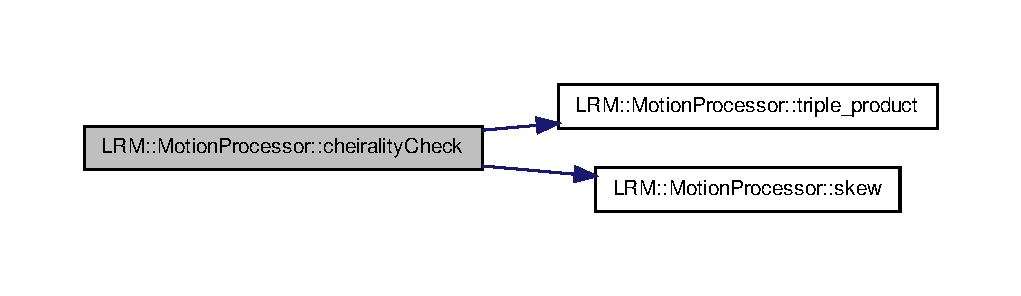
\includegraphics[width=350pt]{classLRM_1_1MotionProcessor_a6d556c3dd5d0c682c407e65b51e2207e_cgraph}
\end{center}
\end{figure}


\hypertarget{classLRM_1_1MotionProcessor_aa06b8d787d57f51f99a0281582a136bc}{\index{\-L\-R\-M\-::\-Motion\-Processor@{\-L\-R\-M\-::\-Motion\-Processor}!compute\-\_\-\-F\-\_\-matrix@{compute\-\_\-\-F\-\_\-matrix}}
\index{compute\-\_\-\-F\-\_\-matrix@{compute\-\_\-\-F\-\_\-matrix}!LRM::MotionProcessor@{\-L\-R\-M\-::\-Motion\-Processor}}
\subsubsection[{compute\-\_\-\-F\-\_\-matrix}]{\setlength{\rightskip}{0pt plus 5cm}cv\-::\-Mat {\bf \-L\-R\-M\-::\-Motion\-Processor\-::compute\-\_\-\-F\-\_\-matrix} (
\begin{DoxyParamCaption}
\item[{std\-::vector$<$ cv\-::\-Point2d $>$}]{train\-\_\-pts, }
\item[{std\-::vector$<$ cv\-::\-Point2d $>$}]{query\-\_\-pts}
\end{DoxyParamCaption}
)}}\label{classLRM_1_1MotionProcessor_aa06b8d787d57f51f99a0281582a136bc}
\hypertarget{classLRM_1_1MotionProcessor_af5cedadc3cafc249f88012884909b138}{\index{\-L\-R\-M\-::\-Motion\-Processor@{\-L\-R\-M\-::\-Motion\-Processor}!compute\-\_\-\-Rt@{compute\-\_\-\-Rt}}
\index{compute\-\_\-\-Rt@{compute\-\_\-\-Rt}!LRM::MotionProcessor@{\-L\-R\-M\-::\-Motion\-Processor}}
\subsubsection[{compute\-\_\-\-Rt}]{\setlength{\rightskip}{0pt plus 5cm}std\-::vector$<$ cv\-::\-Mat $>$ {\bf \-L\-R\-M\-::\-Motion\-Processor\-::compute\-\_\-\-Rt} (
\begin{DoxyParamCaption}
\item[{cv\-::\-Mat}]{\-E, }
\item[{cv\-::\-Mat}]{\-K}
\end{DoxyParamCaption}
)}}\label{classLRM_1_1MotionProcessor_af5cedadc3cafc249f88012884909b138}
\hypertarget{classLRM_1_1MotionProcessor_a13ac0902eb981cacc1dee1a2d586362d}{\index{\-L\-R\-M\-::\-Motion\-Processor@{\-L\-R\-M\-::\-Motion\-Processor}!estimate\-\_\-motion@{estimate\-\_\-motion}}
\index{estimate\-\_\-motion@{estimate\-\_\-motion}!LRM::MotionProcessor@{\-L\-R\-M\-::\-Motion\-Processor}}
\subsubsection[{estimate\-\_\-motion}]{\setlength{\rightskip}{0pt plus 5cm}void {\bf \-L\-R\-M\-::\-Motion\-Processor\-::estimate\-\_\-motion} (
\begin{DoxyParamCaption}
\item[{std\-::vector$<$ cv\-::\-Point2d $>$}]{train\-\_\-pts, }
\item[{std\-::vector$<$ cv\-::\-Point2d $>$}]{query\-\_\-pts, }
\item[{std\-::vector$<$ cv\-::\-D\-Match $>$}]{matches, }
\item[{cv\-::\-Mat}]{\-K}
\end{DoxyParamCaption}
)}}\label{classLRM_1_1MotionProcessor_a13ac0902eb981cacc1dee1a2d586362d}


\-Estimates the rotation and translation between two frames. 


\begin{DoxyParams}{\-Parameters}
{\em train\-\_\-pts} & \-Previous image feature points. \\
\hline
{\em query\-\_\-pts} & \-Current image feature points. \\
\hline
{\em matches} & \-Matches previous and current feature points indexers. \\
\hline
{\em \-K} & \-Intrinsic parameters matrix. \\
\hline
\end{DoxyParams}


\-Here is the call graph for this function\-:\nopagebreak
\begin{figure}[H]
\begin{center}
\leavevmode
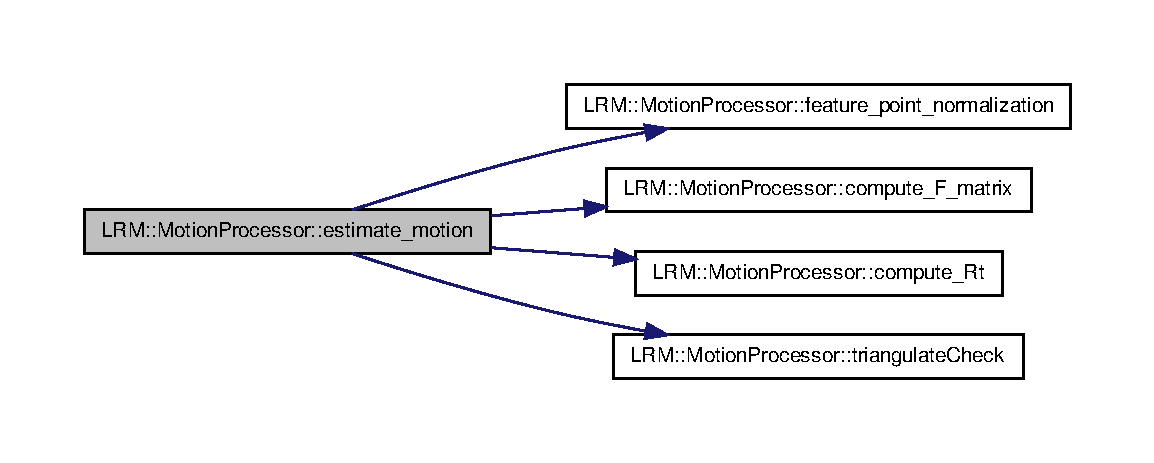
\includegraphics[width=350pt]{classLRM_1_1MotionProcessor_a13ac0902eb981cacc1dee1a2d586362d_cgraph}
\end{center}
\end{figure}


\hypertarget{classLRM_1_1MotionProcessor_aa5cf91a28041e8897469a9ba9bd4b35b}{\index{\-L\-R\-M\-::\-Motion\-Processor@{\-L\-R\-M\-::\-Motion\-Processor}!feature\-\_\-point\-\_\-normalization@{feature\-\_\-point\-\_\-normalization}}
\index{feature\-\_\-point\-\_\-normalization@{feature\-\_\-point\-\_\-normalization}!LRM::MotionProcessor@{\-L\-R\-M\-::\-Motion\-Processor}}
\subsubsection[{feature\-\_\-point\-\_\-normalization}]{\setlength{\rightskip}{0pt plus 5cm}bool {\bf \-L\-R\-M\-::\-Motion\-Processor\-::feature\-\_\-point\-\_\-normalization} (
\begin{DoxyParamCaption}
\item[{std\-::vector$<$ cv\-::\-Point2d $>$}]{query\-\_\-pts, }
\item[{std\-::vector$<$ cv\-::\-Point2d $>$}]{train\-\_\-pts, }
\item[{std\-::vector$<$ cv\-::\-Point2d $>$ \&}]{norm\-\_\-query\-\_\-pts, }
\item[{std\-::vector$<$ cv\-::\-Point2d $>$ \&}]{norm\-\_\-train\-\_\-pts, }
\item[{cv\-::\-Mat \&}]{\-Tc, }
\item[{cv\-::\-Mat \&}]{\-Tp}
\end{DoxyParamCaption}
)}}\label{classLRM_1_1MotionProcessor_aa5cf91a28041e8897469a9ba9bd4b35b}
\hypertarget{classLRM_1_1MotionProcessor_a8029258b4e6d79233b7340eb7695b4f0}{\index{\-L\-R\-M\-::\-Motion\-Processor@{\-L\-R\-M\-::\-Motion\-Processor}!get\-Camera\-Matrix@{get\-Camera\-Matrix}}
\index{get\-Camera\-Matrix@{get\-Camera\-Matrix}!LRM::MotionProcessor@{\-L\-R\-M\-::\-Motion\-Processor}}
\subsubsection[{get\-Camera\-Matrix}]{\setlength{\rightskip}{0pt plus 5cm}cv\-::\-Mat {\bf \-L\-R\-M\-::\-Motion\-Processor\-::get\-Camera\-Matrix} (
\begin{DoxyParamCaption}
{}
\end{DoxyParamCaption}
)\hspace{0.3cm}{\ttfamily  \mbox{[}inline\mbox{]}}}}\label{classLRM_1_1MotionProcessor_a8029258b4e6d79233b7340eb7695b4f0}
\hypertarget{classLRM_1_1MotionProcessor_afea20e7bd776f189fabdd259c22e6b4e}{\index{\-L\-R\-M\-::\-Motion\-Processor@{\-L\-R\-M\-::\-Motion\-Processor}!get\-Inlier\-Mask@{get\-Inlier\-Mask}}
\index{get\-Inlier\-Mask@{get\-Inlier\-Mask}!LRM::MotionProcessor@{\-L\-R\-M\-::\-Motion\-Processor}}
\subsubsection[{get\-Inlier\-Mask}]{\setlength{\rightskip}{0pt plus 5cm}std\-::vector$<$char$>$ {\bf \-L\-R\-M\-::\-Motion\-Processor\-::get\-Inlier\-Mask} (
\begin{DoxyParamCaption}
{}
\end{DoxyParamCaption}
)\hspace{0.3cm}{\ttfamily  \mbox{[}inline\mbox{]}}}}\label{classLRM_1_1MotionProcessor_afea20e7bd776f189fabdd259c22e6b4e}
\hypertarget{classLRM_1_1MotionProcessor_a2fa4b7f533a12a88058a63b87ad96f4a}{\index{\-L\-R\-M\-::\-Motion\-Processor@{\-L\-R\-M\-::\-Motion\-Processor}!matches2points@{matches2points}}
\index{matches2points@{matches2points}!LRM::MotionProcessor@{\-L\-R\-M\-::\-Motion\-Processor}}
\subsubsection[{matches2points}]{\setlength{\rightskip}{0pt plus 5cm}void {\bf \-L\-R\-M\-::\-Motion\-Processor\-::matches2points} (
\begin{DoxyParamCaption}
\item[{const std\-::vector$<$ cv\-::\-Key\-Point $>$ \&}]{query, }
\item[{const std\-::vector$<$ cv\-::\-Key\-Point $>$ \&}]{train, }
\item[{const std\-::vector$<$ cv\-::\-D\-Match $>$ \&}]{matches, }
\item[{std\-::vector$<$ cv\-::\-Point2d $>$ \&}]{query\-\_\-pts, }
\item[{std\-::vector$<$ cv\-::\-Point2d $>$ \&}]{train\-\_\-pts}
\end{DoxyParamCaption}
)}}\label{classLRM_1_1MotionProcessor_a2fa4b7f533a12a88058a63b87ad96f4a}
matches2points\-: \-Tranform the keypoints matched in a matched list of points.


\begin{DoxyParams}{\-Parameters}
{\em query} & \-Current set of keypoints. \\
\hline
{\em train} & \-Last set of keypoints. \\
\hline
{\em matches} & \-Matches between the current and last keypoints. \\
\hline
{\em query\-\_\-pts} & \-Current set of 2\-D points. \\
\hline
{\em train\-\_\-pts} & \-Last set of 2\-D points. \\
\hline
\end{DoxyParams}
\hypertarget{classLRM_1_1MotionProcessor_a848e86c9fc94cf58de7c4f6ae7e50267}{\index{\-L\-R\-M\-::\-Motion\-Processor@{\-L\-R\-M\-::\-Motion\-Processor}!\-Rodrigues@{\-Rodrigues}}
\index{\-Rodrigues@{\-Rodrigues}!LRM::MotionProcessor@{\-L\-R\-M\-::\-Motion\-Processor}}
\subsubsection[{\-Rodrigues}]{\setlength{\rightskip}{0pt plus 5cm}cv\-::\-Mat {\bf \-L\-R\-M\-::\-Motion\-Processor\-::\-Rodrigues} (
\begin{DoxyParamCaption}
\item[{cv\-::\-Vec3d}]{omega, }
\item[{double}]{theta = {\ttfamily -\/1}}
\end{DoxyParamCaption}
)}}\label{classLRM_1_1MotionProcessor_a848e86c9fc94cf58de7c4f6ae7e50267}
\hypertarget{classLRM_1_1MotionProcessor_a64c33eeeac78f7f8358c77daa4635689}{\index{\-L\-R\-M\-::\-Motion\-Processor@{\-L\-R\-M\-::\-Motion\-Processor}!setting@{setting}}
\index{setting@{setting}!LRM::MotionProcessor@{\-L\-R\-M\-::\-Motion\-Processor}}
\subsubsection[{setting}]{\setlength{\rightskip}{0pt plus 5cm}int {\bf \-L\-R\-M\-::\-Motion\-Processor\-::setting} (
\begin{DoxyParamCaption}
\item[{{\bf \-Motion\-Processor\-Parameter}}]{param}
\end{DoxyParamCaption}
)}}\label{classLRM_1_1MotionProcessor_a64c33eeeac78f7f8358c77daa4635689}


\-Here is the call graph for this function\-:\nopagebreak
\begin{figure}[H]
\begin{center}
\leavevmode
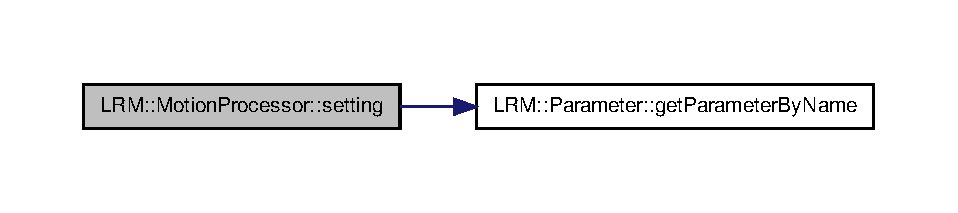
\includegraphics[width=350pt]{classLRM_1_1MotionProcessor_a64c33eeeac78f7f8358c77daa4635689_cgraph}
\end{center}
\end{figure}


\hypertarget{classLRM_1_1MotionProcessor_a3254a463388e2a6db96e81aa29f5b72e}{\index{\-L\-R\-M\-::\-Motion\-Processor@{\-L\-R\-M\-::\-Motion\-Processor}!skew@{skew}}
\index{skew@{skew}!LRM::MotionProcessor@{\-L\-R\-M\-::\-Motion\-Processor}}
\subsubsection[{skew}]{\setlength{\rightskip}{0pt plus 5cm}cv\-::\-Mat {\bf \-L\-R\-M\-::\-Motion\-Processor\-::skew} (
\begin{DoxyParamCaption}
\item[{cv\-::\-Vec3d}]{a}
\end{DoxyParamCaption}
)}}\label{classLRM_1_1MotionProcessor_a3254a463388e2a6db96e81aa29f5b72e}
\hypertarget{classLRM_1_1MotionProcessor_a14ef29f158bf0fe19d05dbadc81e64a0}{\index{\-L\-R\-M\-::\-Motion\-Processor@{\-L\-R\-M\-::\-Motion\-Processor}!triangulate\-Check@{triangulate\-Check}}
\index{triangulate\-Check@{triangulate\-Check}!LRM::MotionProcessor@{\-L\-R\-M\-::\-Motion\-Processor}}
\subsubsection[{triangulate\-Check}]{\setlength{\rightskip}{0pt plus 5cm}int {\bf \-L\-R\-M\-::\-Motion\-Processor\-::triangulate\-Check} (
\begin{DoxyParamCaption}
\item[{std\-::vector$<$ cv\-::\-Point2d $>$}]{train\-\_\-pts, }
\item[{std\-::vector$<$ cv\-::\-Point2d $>$}]{query\-\_\-pts, }
\item[{cv\-::\-Mat \&}]{\-K, }
\item[{cv\-::\-Mat}]{\-P, }
\item[{std\-::vector$<$ char $>$}]{mask = {\ttfamily std\-:\-:vector$<$char$>$()}}
\end{DoxyParamCaption}
)}}\label{classLRM_1_1MotionProcessor_a14ef29f158bf0fe19d05dbadc81e64a0}
\hypertarget{classLRM_1_1MotionProcessor_ac0000e0136ca3c117f1fc548b72d9912}{\index{\-L\-R\-M\-::\-Motion\-Processor@{\-L\-R\-M\-::\-Motion\-Processor}!triple\-\_\-product@{triple\-\_\-product}}
\index{triple\-\_\-product@{triple\-\_\-product}!LRM::MotionProcessor@{\-L\-R\-M\-::\-Motion\-Processor}}
\subsubsection[{triple\-\_\-product}]{\setlength{\rightskip}{0pt plus 5cm}double {\bf \-L\-R\-M\-::\-Motion\-Processor\-::triple\-\_\-product} (
\begin{DoxyParamCaption}
\item[{cv\-::\-Vec3d}]{a, }
\item[{cv\-::\-Vec3d}]{b, }
\item[{cv\-::\-Vec3d}]{c}
\end{DoxyParamCaption}
)}}\label{classLRM_1_1MotionProcessor_ac0000e0136ca3c117f1fc548b72d9912}


\subsection{\-Member \-Data \-Documentation}
\hypertarget{classLRM_1_1MotionProcessor_a0220090264566c5e8bc74bfe62f8e332}{\index{\-L\-R\-M\-::\-Motion\-Processor@{\-L\-R\-M\-::\-Motion\-Processor}!confidence@{confidence}}
\index{confidence@{confidence}!LRM::MotionProcessor@{\-L\-R\-M\-::\-Motion\-Processor}}
\subsubsection[{confidence}]{\setlength{\rightskip}{0pt plus 5cm}double {\bf \-L\-R\-M\-::\-Motion\-Processor\-::confidence}\hspace{0.3cm}{\ttfamily  \mbox{[}private\mbox{]}}}}\label{classLRM_1_1MotionProcessor_a0220090264566c5e8bc74bfe62f8e332}
\hypertarget{classLRM_1_1MotionProcessor_ac18eb15f6b48e4e7f00557e2df1cfb3a}{\index{\-L\-R\-M\-::\-Motion\-Processor@{\-L\-R\-M\-::\-Motion\-Processor}!epipolar\-\_\-dist@{epipolar\-\_\-dist}}
\index{epipolar\-\_\-dist@{epipolar\-\_\-dist}!LRM::MotionProcessor@{\-L\-R\-M\-::\-Motion\-Processor}}
\subsubsection[{epipolar\-\_\-dist}]{\setlength{\rightskip}{0pt plus 5cm}double {\bf \-L\-R\-M\-::\-Motion\-Processor\-::epipolar\-\_\-dist}\hspace{0.3cm}{\ttfamily  \mbox{[}private\mbox{]}}}}\label{classLRM_1_1MotionProcessor_ac18eb15f6b48e4e7f00557e2df1cfb3a}
\hypertarget{classLRM_1_1MotionProcessor_a1cebe392055fdfe8002def6c7810f754}{\index{\-L\-R\-M\-::\-Motion\-Processor@{\-L\-R\-M\-::\-Motion\-Processor}!inliers@{inliers}}
\index{inliers@{inliers}!LRM::MotionProcessor@{\-L\-R\-M\-::\-Motion\-Processor}}
\subsubsection[{inliers}]{\setlength{\rightskip}{0pt plus 5cm}std\-::vector$<$char$>$ {\bf \-L\-R\-M\-::\-Motion\-Processor\-::inliers}\hspace{0.3cm}{\ttfamily  \mbox{[}private\mbox{]}}}}\label{classLRM_1_1MotionProcessor_a1cebe392055fdfe8002def6c7810f754}
\hypertarget{classLRM_1_1MotionProcessor_a84d9c7cce3207b43bb79988c32d07f23}{\index{\-L\-R\-M\-::\-Motion\-Processor@{\-L\-R\-M\-::\-Motion\-Processor}!\-P@{\-P}}
\index{\-P@{\-P}!LRM::MotionProcessor@{\-L\-R\-M\-::\-Motion\-Processor}}
\subsubsection[{\-P}]{\setlength{\rightskip}{0pt plus 5cm}cv\-::\-Mat {\bf \-L\-R\-M\-::\-Motion\-Processor\-::\-P}\hspace{0.3cm}{\ttfamily  \mbox{[}private\mbox{]}}}}\label{classLRM_1_1MotionProcessor_a84d9c7cce3207b43bb79988c32d07f23}
\hypertarget{classLRM_1_1MotionProcessor_af0e2f9ee5479177b49a6caf44962faff}{\index{\-L\-R\-M\-::\-Motion\-Processor@{\-L\-R\-M\-::\-Motion\-Processor}!query\-\_\-pts@{query\-\_\-pts}}
\index{query\-\_\-pts@{query\-\_\-pts}!LRM::MotionProcessor@{\-L\-R\-M\-::\-Motion\-Processor}}
\subsubsection[{query\-\_\-pts}]{\setlength{\rightskip}{0pt plus 5cm}std\-::vector$<$cv\-::\-Point2d$>$ {\bf \-L\-R\-M\-::\-Motion\-Processor\-::query\-\_\-pts}\hspace{0.3cm}{\ttfamily  \mbox{[}private\mbox{]}}}}\label{classLRM_1_1MotionProcessor_af0e2f9ee5479177b49a6caf44962faff}
\hypertarget{classLRM_1_1MotionProcessor_ae72b3aea2c352caefb7f256a40ca6e31}{\index{\-L\-R\-M\-::\-Motion\-Processor@{\-L\-R\-M\-::\-Motion\-Processor}!train\-\_\-pts@{train\-\_\-pts}}
\index{train\-\_\-pts@{train\-\_\-pts}!LRM::MotionProcessor@{\-L\-R\-M\-::\-Motion\-Processor}}
\subsubsection[{train\-\_\-pts}]{\setlength{\rightskip}{0pt plus 5cm}std\-::vector$<$cv\-::\-Point2d$>$ {\bf \-L\-R\-M\-::\-Motion\-Processor\-::train\-\_\-pts}\hspace{0.3cm}{\ttfamily  \mbox{[}private\mbox{]}}}}\label{classLRM_1_1MotionProcessor_ae72b3aea2c352caefb7f256a40ca6e31}


\-The documentation for this class was generated from the following files\-:\begin{DoxyCompactItemize}
\item 
include/\hyperlink{motion__processor_8h}{motion\-\_\-processor.\-h}\item 
src/\hyperlink{motion__processor_8cpp}{motion\-\_\-processor.\-cpp}\end{DoxyCompactItemize}

\hypertarget{classLRM_1_1MotionProcessorParameter}{\section{\-L\-R\-M\-:\-:\-Motion\-Processor\-Parameter \-Class \-Reference}
\label{classLRM_1_1MotionProcessorParameter}\index{\-L\-R\-M\-::\-Motion\-Processor\-Parameter@{\-L\-R\-M\-::\-Motion\-Processor\-Parameter}}
}


{\ttfamily \#include $<$motion\-\_\-processor.\-h$>$}



\-Inheritance diagram for \-L\-R\-M\-:\-:\-Motion\-Processor\-Parameter\-:\nopagebreak
\begin{figure}[H]
\begin{center}
\leavevmode
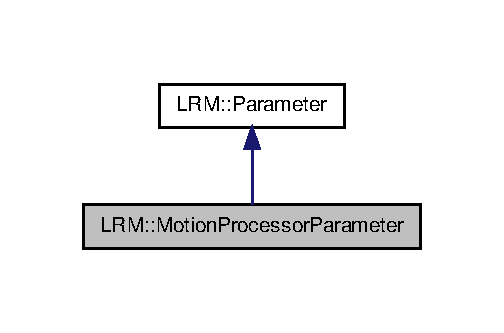
\includegraphics[width=242pt]{classLRM_1_1MotionProcessorParameter__inherit__graph}
\end{center}
\end{figure}


\-Collaboration diagram for \-L\-R\-M\-:\-:\-Motion\-Processor\-Parameter\-:\nopagebreak
\begin{figure}[H]
\begin{center}
\leavevmode
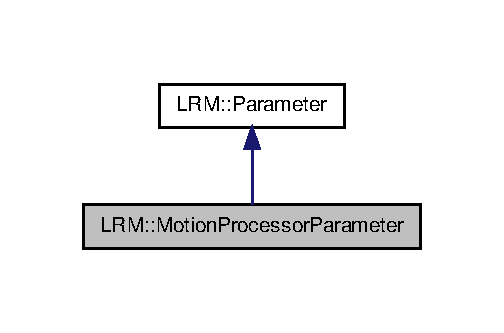
\includegraphics[width=242pt]{classLRM_1_1MotionProcessorParameter__coll__graph}
\end{center}
\end{figure}
\subsection*{\-Public \-Member \-Functions}
\begin{DoxyCompactItemize}
\item 
\hyperlink{classLRM_1_1MotionProcessorParameter_a755180a791ef857695b4484b1e887cfe}{\-Motion\-Processor\-Parameter} ()
\item 
\hyperlink{classLRM_1_1MotionProcessorParameter_a15e756001bbb997a2a7cda443cbcd4bf}{$\sim$\-Motion\-Processor\-Parameter} ()
\item 
int \hyperlink{classLRM_1_1MotionProcessorParameter_a773949b98bb0c02dd8c03f9c74af0481}{parse} (ros\-::\-Node\-Handle nh)
\end{DoxyCompactItemize}


\subsection{\-Detailed \-Description}
\-Motion \-Processor \hyperlink{classLRM_1_1Parameter}{\-Parameter} \-Class 

\subsection{\-Constructor \& \-Destructor \-Documentation}
\hypertarget{classLRM_1_1MotionProcessorParameter_a755180a791ef857695b4484b1e887cfe}{\index{\-L\-R\-M\-::\-Motion\-Processor\-Parameter@{\-L\-R\-M\-::\-Motion\-Processor\-Parameter}!\-Motion\-Processor\-Parameter@{\-Motion\-Processor\-Parameter}}
\index{\-Motion\-Processor\-Parameter@{\-Motion\-Processor\-Parameter}!LRM::MotionProcessorParameter@{\-L\-R\-M\-::\-Motion\-Processor\-Parameter}}
\subsubsection[{\-Motion\-Processor\-Parameter}]{\setlength{\rightskip}{0pt plus 5cm}{\bf \-L\-R\-M\-::\-Motion\-Processor\-Parameter\-::\-Motion\-Processor\-Parameter} (
\begin{DoxyParamCaption}
{}
\end{DoxyParamCaption}
)\hspace{0.3cm}{\ttfamily  \mbox{[}inline\mbox{]}}}}\label{classLRM_1_1MotionProcessorParameter_a755180a791ef857695b4484b1e887cfe}
\hypertarget{classLRM_1_1MotionProcessorParameter_a15e756001bbb997a2a7cda443cbcd4bf}{\index{\-L\-R\-M\-::\-Motion\-Processor\-Parameter@{\-L\-R\-M\-::\-Motion\-Processor\-Parameter}!$\sim$\-Motion\-Processor\-Parameter@{$\sim$\-Motion\-Processor\-Parameter}}
\index{$\sim$\-Motion\-Processor\-Parameter@{$\sim$\-Motion\-Processor\-Parameter}!LRM::MotionProcessorParameter@{\-L\-R\-M\-::\-Motion\-Processor\-Parameter}}
\subsubsection[{$\sim$\-Motion\-Processor\-Parameter}]{\setlength{\rightskip}{0pt plus 5cm}{\bf \-L\-R\-M\-::\-Motion\-Processor\-Parameter\-::$\sim$\-Motion\-Processor\-Parameter} (
\begin{DoxyParamCaption}
{}
\end{DoxyParamCaption}
)\hspace{0.3cm}{\ttfamily  \mbox{[}inline\mbox{]}}}}\label{classLRM_1_1MotionProcessorParameter_a15e756001bbb997a2a7cda443cbcd4bf}


\subsection{\-Member \-Function \-Documentation}
\hypertarget{classLRM_1_1MotionProcessorParameter_a773949b98bb0c02dd8c03f9c74af0481}{\index{\-L\-R\-M\-::\-Motion\-Processor\-Parameter@{\-L\-R\-M\-::\-Motion\-Processor\-Parameter}!parse@{parse}}
\index{parse@{parse}!LRM::MotionProcessorParameter@{\-L\-R\-M\-::\-Motion\-Processor\-Parameter}}
\subsubsection[{parse}]{\setlength{\rightskip}{0pt plus 5cm}int {\bf \-L\-R\-M\-::\-Motion\-Processor\-Parameter\-::parse} (
\begin{DoxyParamCaption}
\item[{ros\-::\-Node\-Handle}]{nh}
\end{DoxyParamCaption}
)\hspace{0.3cm}{\ttfamily  \mbox{[}virtual\mbox{]}}}}\label{classLRM_1_1MotionProcessorParameter_a773949b98bb0c02dd8c03f9c74af0481}
\-Motion \-Processor \hyperlink{classLRM_1_1Parameter}{\-Parameter} \-Class 

\-Implements \hyperlink{classLRM_1_1Parameter_ad53ef22f20e18578caa644866aaa234b}{\-L\-R\-M\-::\-Parameter}.



\-The documentation for this class was generated from the following files\-:\begin{DoxyCompactItemize}
\item 
include/\hyperlink{motion__processor_8h}{motion\-\_\-processor.\-h}\item 
src/\hyperlink{motion__processor_8cpp}{motion\-\_\-processor.\-cpp}\end{DoxyCompactItemize}

\hypertarget{classLRM_1_1Parameter}{\section{\-L\-R\-M\-:\-:\-Parameter \-Class \-Reference}
\label{classLRM_1_1Parameter}\index{\-L\-R\-M\-::\-Parameter@{\-L\-R\-M\-::\-Parameter}}
}


{\ttfamily \#include $<$parameter.\-h$>$}



\-Inheritance diagram for \-L\-R\-M\-:\-:\-Parameter\-:\nopagebreak
\begin{figure}[H]
\begin{center}
\leavevmode
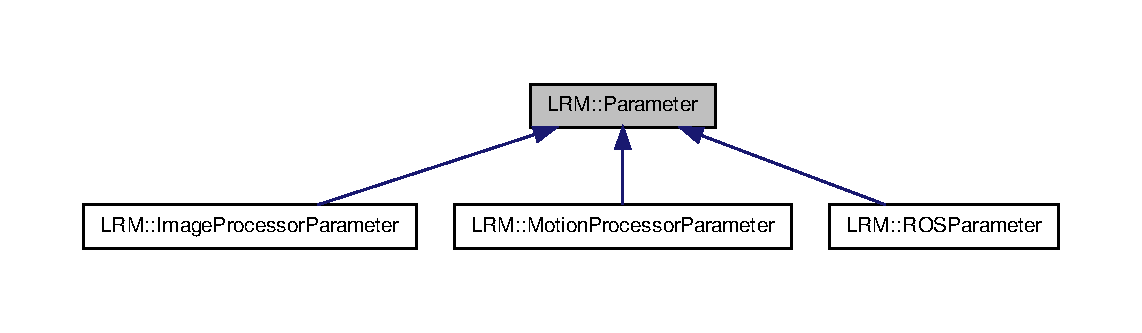
\includegraphics[width=350pt]{classLRM_1_1Parameter__inherit__graph}
\end{center}
\end{figure}
\subsection*{\-Public \-Member \-Functions}
\begin{DoxyCompactItemize}
\item 
\hyperlink{classLRM_1_1Parameter_a1e33c84585b5d4979d4928d3400c7bd5}{\-Parameter} ()
\item 
virtual \hyperlink{classLRM_1_1Parameter_a48ef0a4ad52f8c998081fc7aaee8bcb0}{$\sim$\-Parameter} ()
\item 
virtual int \hyperlink{classLRM_1_1Parameter_ad53ef22f20e18578caa644866aaa234b}{parse} (ros\-::\-Node\-Handle)=0
\item 
{\footnotesize template$<$class T $>$ }\\\-T \hyperlink{classLRM_1_1Parameter_a1e39678803d61a1cfe74b9f2fcc2d847}{get\-Parameter\-By\-Name} (std\-::string name)
\item 
int \hyperlink{classLRM_1_1Parameter_a84b380711eed82a3b58dd9b5f3692f79}{set\-Parameter\-By\-Name} (std\-::string name, boost\-::any value)
\end{DoxyCompactItemize}
\subsection*{\-Protected \-Attributes}
\begin{DoxyCompactItemize}
\item 
std\-::map$<$ std\-::string, boost\-::any $>$ \hyperlink{classLRM_1_1Parameter_ac16ee52d4a330bb21b85a2a01e184da0}{parameter}
\end{DoxyCompactItemize}


\subsection{\-Constructor \& \-Destructor \-Documentation}
\hypertarget{classLRM_1_1Parameter_a1e33c84585b5d4979d4928d3400c7bd5}{\index{\-L\-R\-M\-::\-Parameter@{\-L\-R\-M\-::\-Parameter}!\-Parameter@{\-Parameter}}
\index{\-Parameter@{\-Parameter}!LRM::Parameter@{\-L\-R\-M\-::\-Parameter}}
\subsubsection[{\-Parameter}]{\setlength{\rightskip}{0pt plus 5cm}{\bf \-L\-R\-M\-::\-Parameter\-::\-Parameter} (
\begin{DoxyParamCaption}
{}
\end{DoxyParamCaption}
)\hspace{0.3cm}{\ttfamily  \mbox{[}inline\mbox{]}}}}\label{classLRM_1_1Parameter_a1e33c84585b5d4979d4928d3400c7bd5}
\hypertarget{classLRM_1_1Parameter_a48ef0a4ad52f8c998081fc7aaee8bcb0}{\index{\-L\-R\-M\-::\-Parameter@{\-L\-R\-M\-::\-Parameter}!$\sim$\-Parameter@{$\sim$\-Parameter}}
\index{$\sim$\-Parameter@{$\sim$\-Parameter}!LRM::Parameter@{\-L\-R\-M\-::\-Parameter}}
\subsubsection[{$\sim$\-Parameter}]{\setlength{\rightskip}{0pt plus 5cm}virtual {\bf \-L\-R\-M\-::\-Parameter\-::$\sim$\-Parameter} (
\begin{DoxyParamCaption}
{}
\end{DoxyParamCaption}
)\hspace{0.3cm}{\ttfamily  \mbox{[}inline, virtual\mbox{]}}}}\label{classLRM_1_1Parameter_a48ef0a4ad52f8c998081fc7aaee8bcb0}


\subsection{\-Member \-Function \-Documentation}
\hypertarget{classLRM_1_1Parameter_a1e39678803d61a1cfe74b9f2fcc2d847}{\index{\-L\-R\-M\-::\-Parameter@{\-L\-R\-M\-::\-Parameter}!get\-Parameter\-By\-Name@{get\-Parameter\-By\-Name}}
\index{get\-Parameter\-By\-Name@{get\-Parameter\-By\-Name}!LRM::Parameter@{\-L\-R\-M\-::\-Parameter}}
\subsubsection[{get\-Parameter\-By\-Name}]{\setlength{\rightskip}{0pt plus 5cm}template$<$class T $>$ \-T {\bf \-L\-R\-M\-::\-Parameter\-::get\-Parameter\-By\-Name} (
\begin{DoxyParamCaption}
\item[{std\-::string}]{name}
\end{DoxyParamCaption}
)\hspace{0.3cm}{\ttfamily  \mbox{[}inline\mbox{]}}}}\label{classLRM_1_1Parameter_a1e39678803d61a1cfe74b9f2fcc2d847}
\hypertarget{classLRM_1_1Parameter_ad53ef22f20e18578caa644866aaa234b}{\index{\-L\-R\-M\-::\-Parameter@{\-L\-R\-M\-::\-Parameter}!parse@{parse}}
\index{parse@{parse}!LRM::Parameter@{\-L\-R\-M\-::\-Parameter}}
\subsubsection[{parse}]{\setlength{\rightskip}{0pt plus 5cm}virtual int {\bf \-L\-R\-M\-::\-Parameter\-::parse} (
\begin{DoxyParamCaption}
\item[{ros\-::\-Node\-Handle}]{}
\end{DoxyParamCaption}
)\hspace{0.3cm}{\ttfamily  \mbox{[}pure virtual\mbox{]}}}}\label{classLRM_1_1Parameter_ad53ef22f20e18578caa644866aaa234b}


\-Implemented in \hyperlink{classLRM_1_1ROSParameter_adfd704986bd8a4c12e1139b2a8d08871}{\-L\-R\-M\-::\-R\-O\-S\-Parameter}, \hyperlink{classLRM_1_1MotionProcessorParameter_a773949b98bb0c02dd8c03f9c74af0481}{\-L\-R\-M\-::\-Motion\-Processor\-Parameter}, and \hyperlink{classLRM_1_1ImageProcessorParameter_a381448a39d6b41c8f44fd5b45f975b4a}{\-L\-R\-M\-::\-Image\-Processor\-Parameter}.

\hypertarget{classLRM_1_1Parameter_a84b380711eed82a3b58dd9b5f3692f79}{\index{\-L\-R\-M\-::\-Parameter@{\-L\-R\-M\-::\-Parameter}!set\-Parameter\-By\-Name@{set\-Parameter\-By\-Name}}
\index{set\-Parameter\-By\-Name@{set\-Parameter\-By\-Name}!LRM::Parameter@{\-L\-R\-M\-::\-Parameter}}
\subsubsection[{set\-Parameter\-By\-Name}]{\setlength{\rightskip}{0pt plus 5cm}int {\bf \-L\-R\-M\-::\-Parameter\-::set\-Parameter\-By\-Name} (
\begin{DoxyParamCaption}
\item[{std\-::string}]{name, }
\item[{boost\-::any}]{value}
\end{DoxyParamCaption}
)\hspace{0.3cm}{\ttfamily  \mbox{[}inline\mbox{]}}}}\label{classLRM_1_1Parameter_a84b380711eed82a3b58dd9b5f3692f79}


\subsection{\-Member \-Data \-Documentation}
\hypertarget{classLRM_1_1Parameter_ac16ee52d4a330bb21b85a2a01e184da0}{\index{\-L\-R\-M\-::\-Parameter@{\-L\-R\-M\-::\-Parameter}!parameter@{parameter}}
\index{parameter@{parameter}!LRM::Parameter@{\-L\-R\-M\-::\-Parameter}}
\subsubsection[{parameter}]{\setlength{\rightskip}{0pt plus 5cm}std\-::map$<$std\-::string, boost\-::any$>$ {\bf \-L\-R\-M\-::\-Parameter\-::parameter}\hspace{0.3cm}{\ttfamily  \mbox{[}protected\mbox{]}}}}\label{classLRM_1_1Parameter_ac16ee52d4a330bb21b85a2a01e184da0}


\-The documentation for this class was generated from the following file\-:\begin{DoxyCompactItemize}
\item 
include/\hyperlink{parameter_8h}{parameter.\-h}\end{DoxyCompactItemize}

\hypertarget{classLRM_1_1ROSParameter}{\section{\-L\-R\-M\-:\-:\-R\-O\-S\-Parameter \-Class \-Reference}
\label{classLRM_1_1ROSParameter}\index{\-L\-R\-M\-::\-R\-O\-S\-Parameter@{\-L\-R\-M\-::\-R\-O\-S\-Parameter}}
}


{\ttfamily \#include $<$mono\-\_\-odometer.\-h$>$}



\-Inheritance diagram for \-L\-R\-M\-:\-:\-R\-O\-S\-Parameter\-:\nopagebreak
\begin{figure}[H]
\begin{center}
\leavevmode
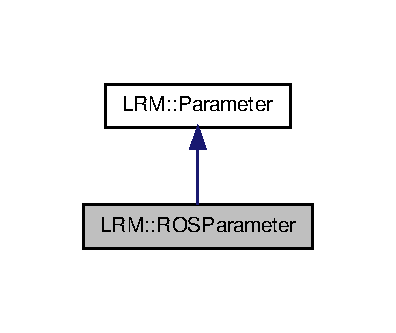
\includegraphics[width=190pt]{classLRM_1_1ROSParameter__inherit__graph}
\end{center}
\end{figure}


\-Collaboration diagram for \-L\-R\-M\-:\-:\-R\-O\-S\-Parameter\-:\nopagebreak
\begin{figure}[H]
\begin{center}
\leavevmode
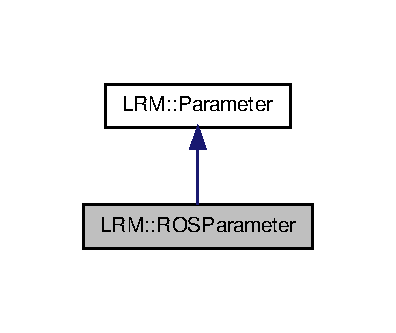
\includegraphics[width=190pt]{classLRM_1_1ROSParameter__coll__graph}
\end{center}
\end{figure}
\subsection*{\-Public \-Member \-Functions}
\begin{DoxyCompactItemize}
\item 
\hyperlink{classLRM_1_1ROSParameter_a1829f2f498ed9baa732c5653a29fa18d}{\-R\-O\-S\-Parameter} ()
\item 
\hyperlink{classLRM_1_1ROSParameter_a858dfa2e9ab046a7dba1699cb712f810}{$\sim$\-R\-O\-S\-Parameter} ()
\item 
int \hyperlink{classLRM_1_1ROSParameter_adfd704986bd8a4c12e1139b2a8d08871}{parse} (ros\-::\-Node\-Handle nh)
\end{DoxyCompactItemize}


\subsection{\-Detailed \-Description}
\-List of parameter regarding \-R\-O\-S configuration for the launch file.
\begin{DoxyItemize}
\item {\bfseries \-I\-N\-T\-R\-I\-N\-S\-I\-C\-\_\-\-M\-A\-T\-R\-I\-X\-\_\-\-P\-A\-T\-H\-:} \-Path to the intrinsic matrix \-K file. ({\bfseries \-File} {\bfseries format\-:\-Y\-A\-M\-L} -\/ {\bfseries \-Default\-:} empty)
\item {\bfseries \-I\-N\-P\-U\-T\-\_\-\-I\-M\-A\-G\-E\-\_\-\-T\-O\-P\-I\-C\-:} \-Topic name of the input image. ({\bfseries \-Default\-:} /camera/image)
\item {\bfseries \-F\-E\-A\-T\-U\-R\-E\-\_\-\-I\-M\-A\-G\-E\-\_\-\-T\-O\-P\-I\-C\-:} \-Name of the topic where the output image with the features detect will be published. ({\bfseries \-Default\-:} images/feature)
\item {\bfseries \-M\-A\-T\-C\-H\-E\-S\-\_\-\-I\-M\-A\-G\-E\-\_\-\-T\-O\-P\-I\-C\-:} \-Name of the topic where the output image with the features matched will be published. ({\bfseries \-Default\-:} images/matches)
\item {\bfseries \-O\-P\-T\-F\-L\-O\-W\-\_\-\-I\-M\-A\-G\-E\-\_\-\-T\-O\-P\-I\-C\-:} \-Name of the topic where the output image with the feature displacement will be published. ({\bfseries \-Default\-:} images/optflow)
\item {\bfseries \-O\-D\-O\-M\-E\-T\-R\-Y\-\_\-\-T\-O\-P\-I\-C\-:} \-Name of the topic where the odometry will be published. ({\bfseries \-Default\-:} odom)
\item {\bfseries \-O\-D\-O\-M\-E\-T\-E\-R\-\_\-\-R\-E\-F\-E\-R\-E\-N\-C\-E\-\_\-\-F\-R\-A\-M\-E\-:} \-Fixed frame used as reference for the odometer. ({\bfseries \-Default\-:} odom)
\item {\bfseries \-R\-O\-B\-O\-T\-\_\-\-F\-R\-A\-M\-E\-:} \-The frame which all sensors are referenced to. \-Usually the base link. ({\bfseries \-Default\-:} base\-\_\-link)
\item {\bfseries \-S\-E\-N\-S\-O\-R\-\_\-\-F\-R\-A\-M\-E\-:} \-The image capturing sensor frame. ({\bfseries \-Default\-:} camera) 
\end{DoxyItemize}

\subsection{\-Constructor \& \-Destructor \-Documentation}
\hypertarget{classLRM_1_1ROSParameter_a1829f2f498ed9baa732c5653a29fa18d}{\index{\-L\-R\-M\-::\-R\-O\-S\-Parameter@{\-L\-R\-M\-::\-R\-O\-S\-Parameter}!\-R\-O\-S\-Parameter@{\-R\-O\-S\-Parameter}}
\index{\-R\-O\-S\-Parameter@{\-R\-O\-S\-Parameter}!LRM::ROSParameter@{\-L\-R\-M\-::\-R\-O\-S\-Parameter}}
\subsubsection[{\-R\-O\-S\-Parameter}]{\setlength{\rightskip}{0pt plus 5cm}{\bf \-L\-R\-M\-::\-R\-O\-S\-Parameter\-::\-R\-O\-S\-Parameter} (
\begin{DoxyParamCaption}
{}
\end{DoxyParamCaption}
)\hspace{0.3cm}{\ttfamily  \mbox{[}inline\mbox{]}}}}\label{classLRM_1_1ROSParameter_a1829f2f498ed9baa732c5653a29fa18d}
\hypertarget{classLRM_1_1ROSParameter_a858dfa2e9ab046a7dba1699cb712f810}{\index{\-L\-R\-M\-::\-R\-O\-S\-Parameter@{\-L\-R\-M\-::\-R\-O\-S\-Parameter}!$\sim$\-R\-O\-S\-Parameter@{$\sim$\-R\-O\-S\-Parameter}}
\index{$\sim$\-R\-O\-S\-Parameter@{$\sim$\-R\-O\-S\-Parameter}!LRM::ROSParameter@{\-L\-R\-M\-::\-R\-O\-S\-Parameter}}
\subsubsection[{$\sim$\-R\-O\-S\-Parameter}]{\setlength{\rightskip}{0pt plus 5cm}{\bf \-L\-R\-M\-::\-R\-O\-S\-Parameter\-::$\sim$\-R\-O\-S\-Parameter} (
\begin{DoxyParamCaption}
{}
\end{DoxyParamCaption}
)\hspace{0.3cm}{\ttfamily  \mbox{[}inline\mbox{]}}}}\label{classLRM_1_1ROSParameter_a858dfa2e9ab046a7dba1699cb712f810}


\subsection{\-Member \-Function \-Documentation}
\hypertarget{classLRM_1_1ROSParameter_adfd704986bd8a4c12e1139b2a8d08871}{\index{\-L\-R\-M\-::\-R\-O\-S\-Parameter@{\-L\-R\-M\-::\-R\-O\-S\-Parameter}!parse@{parse}}
\index{parse@{parse}!LRM::ROSParameter@{\-L\-R\-M\-::\-R\-O\-S\-Parameter}}
\subsubsection[{parse}]{\setlength{\rightskip}{0pt plus 5cm}int {\bf \-L\-R\-M\-::\-R\-O\-S\-Parameter\-::parse} (
\begin{DoxyParamCaption}
\item[{ros\-::\-Node\-Handle}]{nh}
\end{DoxyParamCaption}
)\hspace{0.3cm}{\ttfamily  \mbox{[}virtual\mbox{]}}}}\label{classLRM_1_1ROSParameter_adfd704986bd8a4c12e1139b2a8d08871}
\-R\-O\-S \hyperlink{classLRM_1_1Parameter}{\-Parameter} \-Class 

\-Implements \hyperlink{classLRM_1_1Parameter_ad53ef22f20e18578caa644866aaa234b}{\-L\-R\-M\-::\-Parameter}.



\-The documentation for this class was generated from the following files\-:\begin{DoxyCompactItemize}
\item 
include/\hyperlink{mono__odometer_8h}{mono\-\_\-odometer.\-h}\item 
src/\hyperlink{mono__odometer_8cpp}{mono\-\_\-odometer.\-cpp}\end{DoxyCompactItemize}

\chapter{\-File \-Documentation}
\hypertarget{core_8h}{\section{include/core.h \-File \-Reference}
\label{core_8h}\index{include/core.\-h@{include/core.\-h}}
}
{\ttfamily \#include $<$ros/ros.\-h$>$}\*
{\ttfamily \#include $<$sensor\-\_\-msgs/\-Image.\-h$>$}\*
{\ttfamily \#include $<$sensor\-\_\-msgs/image\-\_\-encodings.\-h$>$}\*
{\ttfamily \#include $<$tf/transform\-\_\-broadcaster.\-h$>$}\*
{\ttfamily \#include $<$tf/transform\-\_\-listener.\-h$>$}\*
{\ttfamily \#include $<$nav\-\_\-msgs/\-Odometry.\-h$>$}\*
{\ttfamily \#include $<$geometry\-\_\-msgs/\-Pose\-Stamped.\-h$>$}\*
{\ttfamily \#include $<$cv\-\_\-bridge/cv\-\_\-bridge.\-h$>$}\*
{\ttfamily \#include $<$image\-\_\-transport/image\-\_\-transport.\-h$>$}\*
{\ttfamily \#include $<$opencv2/core/core.\-hpp$>$}\*
{\ttfamily \#include $<$opencv2/imgproc/imgproc.\-hpp$>$}\*
{\ttfamily \#include $<$opencv2/highgui/highgui.\-hpp$>$}\*
{\ttfamily \#include $<$opencv2/features2d/features2d.\-hpp$>$}\*
{\ttfamily \#include $<$opencv2/nonfree/features2d.\-hpp$>$}\*
{\ttfamily \#include $<$opencv2/calib3d/calib3d.\-hpp$>$}\*
{\ttfamily \#include $<$boost/smart\-\_\-ptr.\-hpp$>$}\*
{\ttfamily \#include $<$algorithm$>$}\*
{\ttfamily \#include $<$vector$>$}\*
{\ttfamily \#include $<$deque$>$}\*
\-Include dependency graph for core.\-h\-:\nopagebreak
\begin{figure}[H]
\begin{center}
\leavevmode
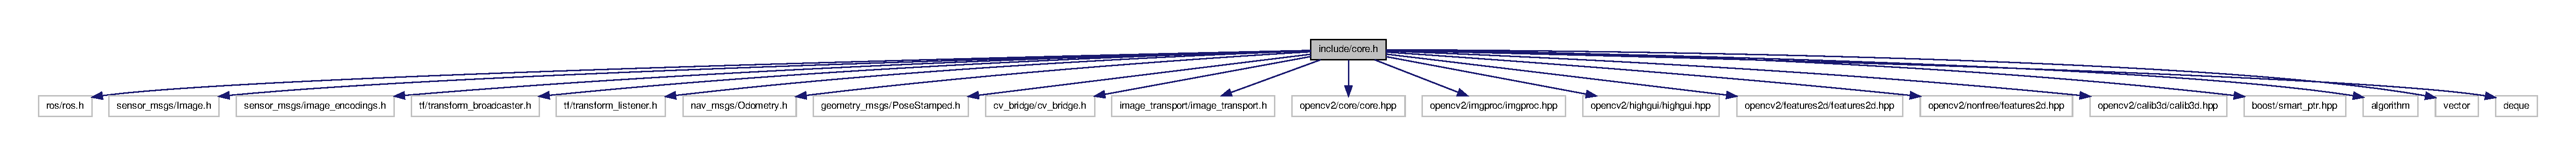
\includegraphics[width=350pt]{core_8h__incl}
\end{center}
\end{figure}
\-This graph shows which files directly or indirectly include this file\-:\nopagebreak
\begin{figure}[H]
\begin{center}
\leavevmode
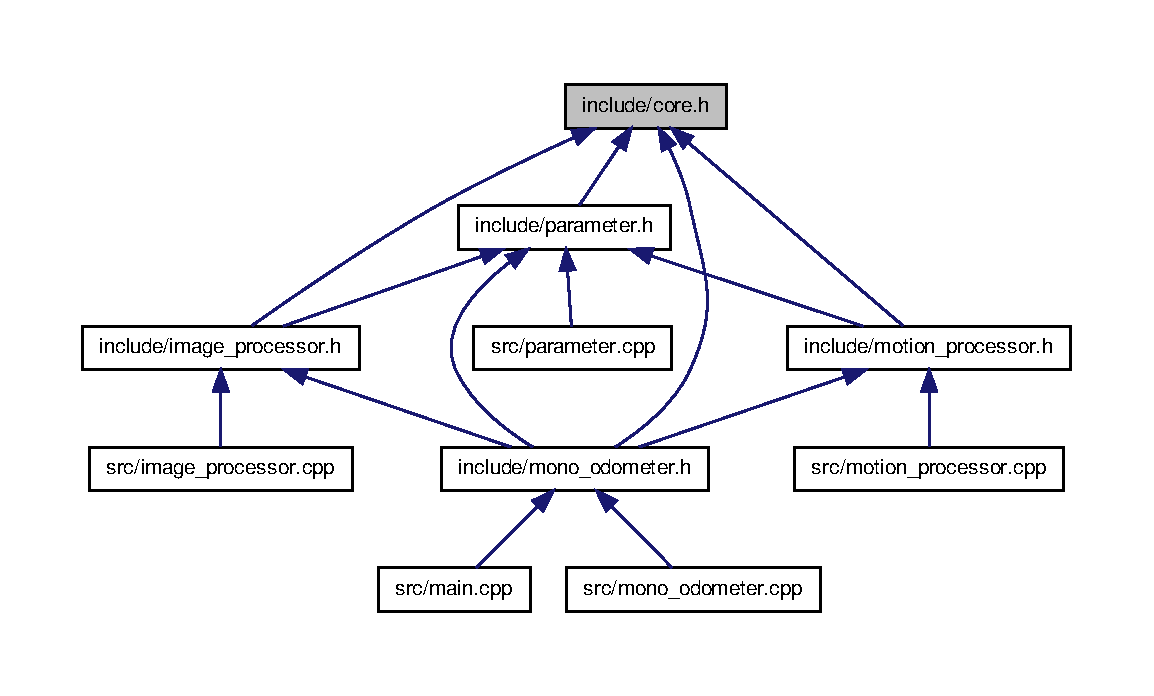
\includegraphics[width=350pt]{core_8h__dep__incl}
\end{center}
\end{figure}
\subsection*{\-Classes}
\begin{DoxyCompactItemize}
\item 
class \hyperlink{classLRM_1_1Feature}{\-L\-R\-M\-::\-Feature}
\end{DoxyCompactItemize}
\subsection*{\-Namespaces}
\begin{DoxyCompactItemize}
\item 
namespace \hyperlink{namespaceLRM}{\-L\-R\-M}
\end{DoxyCompactItemize}
\subsection*{\-Enumerations}
\begin{DoxyCompactItemize}
\item 
enum \hyperlink{namespaceLRM_a8eb6956b84fb7d27bce5af771937794f}{\-L\-R\-M\-::feature\-\_\-t} \{ \*
\hyperlink{namespaceLRM_a8eb6956b84fb7d27bce5af771937794fa8e3a2d26370c85d7adb97cbbd40abc72}{\-L\-R\-M\-::\-S\-H\-I\-\_\-\-T\-O\-M\-A\-S\-I}, 
\hyperlink{namespaceLRM_a8eb6956b84fb7d27bce5af771937794fa82f8a835c4a989b4beddacd8082dc75d}{\-L\-R\-M\-::\-H\-A\-R\-R\-I\-S}, 
\hyperlink{namespaceLRM_a8eb6956b84fb7d27bce5af771937794fa7c70db53c6ef257d06ad41cd33ea8c42}{\-L\-R\-M\-::\-O\-R\-B}, 
\hyperlink{namespaceLRM_a8eb6956b84fb7d27bce5af771937794fa68bc6d3980e55f5e357855916be07ab9}{\-L\-R\-M\-::\-F\-A\-S\-T}, 
\*
\hyperlink{namespaceLRM_a8eb6956b84fb7d27bce5af771937794fabace5d3a329784433515af3067c3e9d9}{\-L\-R\-M\-::\-S\-U\-R\-F}, 
\hyperlink{namespaceLRM_a8eb6956b84fb7d27bce5af771937794fab88abdea089ea29c5224698eb2215891}{\-L\-R\-M\-::\-S\-I\-F\-T}, 
\hyperlink{namespaceLRM_a8eb6956b84fb7d27bce5af771937794faa8a3283e5421c1218d8238e56c80a104}{\-L\-R\-M\-::\-N\-O\-\_\-\-F\-E\-A\-T\-U\-R\-E}
 \}
\begin{DoxyCompactList}\small\item\em \-Types of possible features. \end{DoxyCompactList}\item 
enum \hyperlink{namespaceLRM_ad31d475a7f32e1bd208beb34aabc6fa9}{\-L\-R\-M\-::descriptor\-\_\-t} \{ \hyperlink{namespaceLRM_ad31d475a7f32e1bd208beb34aabc6fa9a1e43a18048d2fc5fc782f2eebce0d585}{\-L\-R\-M\-::\-S\-S\-D}
 \}
\begin{DoxyCompactList}\small\item\em \-Types of possible descriptors. \end{DoxyCompactList}\end{DoxyCompactItemize}

\hypertarget{image__processor_8h}{\section{include/image\-\_\-processor.h \-File \-Reference}
\label{image__processor_8h}\index{include/image\-\_\-processor.\-h@{include/image\-\_\-processor.\-h}}
}
{\ttfamily \#include \char`\"{}core.\-h\char`\"{}}\*
{\ttfamily \#include \char`\"{}parameter.\-h\char`\"{}}\*
\-Include dependency graph for image\-\_\-processor.\-h\-:\nopagebreak
\begin{figure}[H]
\begin{center}
\leavevmode
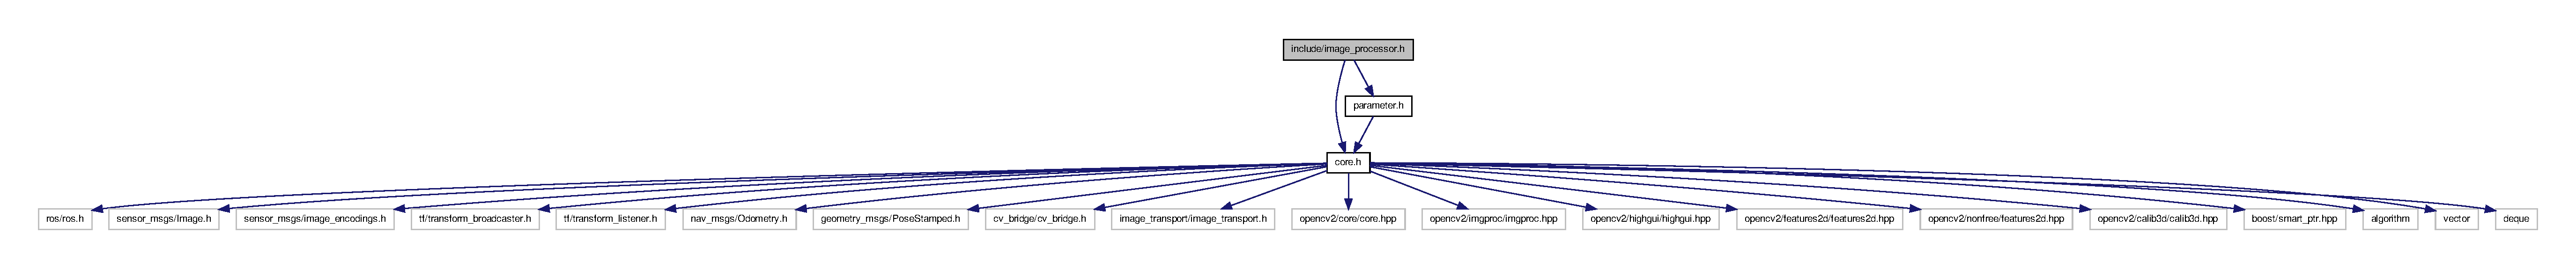
\includegraphics[width=350pt]{image__processor_8h__incl}
\end{center}
\end{figure}
\-This graph shows which files directly or indirectly include this file\-:\nopagebreak
\begin{figure}[H]
\begin{center}
\leavevmode
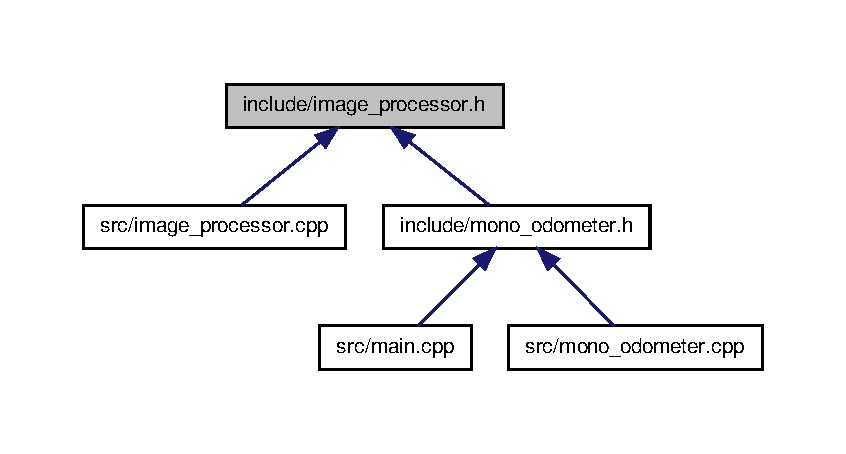
\includegraphics[width=350pt]{image__processor_8h__dep__incl}
\end{center}
\end{figure}
\subsection*{\-Classes}
\begin{DoxyCompactItemize}
\item 
class \hyperlink{classLRM_1_1ImageProcessorParameter}{\-L\-R\-M\-::\-Image\-Processor\-Parameter}
\item 
class \hyperlink{classLRM_1_1ImageProcessor}{\-L\-R\-M\-::\-Image\-Processor}
\end{DoxyCompactItemize}
\subsection*{\-Namespaces}
\begin{DoxyCompactItemize}
\item 
namespace \hyperlink{namespaceLRM}{\-L\-R\-M}
\end{DoxyCompactItemize}
\subsection*{\-Defines}
\begin{DoxyCompactItemize}
\item 
\#define \hyperlink{image__processor_8h_afd1ca313bdba9ff49bf0c988482d7bc5}{\-D\-E\-F\-A\-U\-L\-T\-\_\-\-R\-A\-D\-I\-U\-S}~10.\-0
\end{DoxyCompactItemize}


\subsection{\-Define \-Documentation}
\hypertarget{image__processor_8h_afd1ca313bdba9ff49bf0c988482d7bc5}{\index{image\-\_\-processor.\-h@{image\-\_\-processor.\-h}!\-D\-E\-F\-A\-U\-L\-T\-\_\-\-R\-A\-D\-I\-U\-S@{\-D\-E\-F\-A\-U\-L\-T\-\_\-\-R\-A\-D\-I\-U\-S}}
\index{\-D\-E\-F\-A\-U\-L\-T\-\_\-\-R\-A\-D\-I\-U\-S@{\-D\-E\-F\-A\-U\-L\-T\-\_\-\-R\-A\-D\-I\-U\-S}!image_processor.h@{image\-\_\-processor.\-h}}
\subsubsection[{\-D\-E\-F\-A\-U\-L\-T\-\_\-\-R\-A\-D\-I\-U\-S}]{\setlength{\rightskip}{0pt plus 5cm}\#define {\bf \-D\-E\-F\-A\-U\-L\-T\-\_\-\-R\-A\-D\-I\-U\-S}~10.\-0}}\label{image__processor_8h_afd1ca313bdba9ff49bf0c988482d7bc5}

\hypertarget{mono__odometer_8h}{\section{include/mono\-\_\-odometer.h \-File \-Reference}
\label{mono__odometer_8h}\index{include/mono\-\_\-odometer.\-h@{include/mono\-\_\-odometer.\-h}}
}
{\ttfamily \#include \char`\"{}core.\-h\char`\"{}}\*
{\ttfamily \#include \char`\"{}parameter.\-h\char`\"{}}\*
{\ttfamily \#include \char`\"{}image\-\_\-processor.\-h\char`\"{}}\*
{\ttfamily \#include \char`\"{}motion\-\_\-processor.\-h\char`\"{}}\*
{\ttfamily \#include $<$fstream$>$}\*
\-Include dependency graph for mono\-\_\-odometer.\-h\-:\nopagebreak
\begin{figure}[H]
\begin{center}
\leavevmode
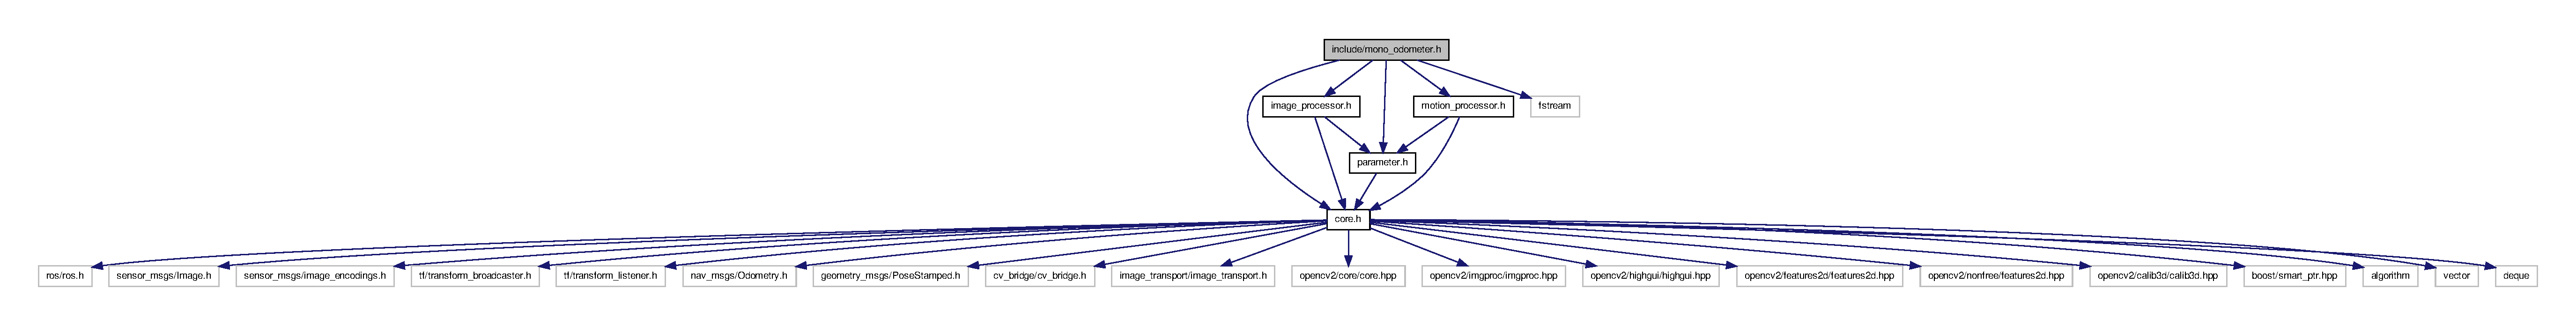
\includegraphics[width=350pt]{mono__odometer_8h__incl}
\end{center}
\end{figure}
\-This graph shows which files directly or indirectly include this file\-:\nopagebreak
\begin{figure}[H]
\begin{center}
\leavevmode
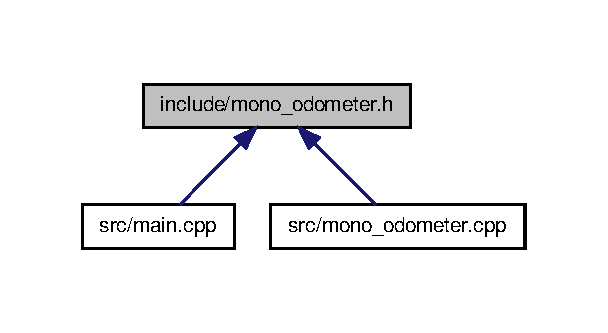
\includegraphics[width=292pt]{mono__odometer_8h__dep__incl}
\end{center}
\end{figure}
\subsection*{\-Classes}
\begin{DoxyCompactItemize}
\item 
class \hyperlink{classLRM_1_1ROSParameter}{\-L\-R\-M\-::\-R\-O\-S\-Parameter}
\item 
class \hyperlink{classLRM_1_1MonoOdometer}{\-L\-R\-M\-::\-Mono\-Odometer}
\end{DoxyCompactItemize}
\subsection*{\-Namespaces}
\begin{DoxyCompactItemize}
\item 
namespace \hyperlink{namespaceLRM}{\-L\-R\-M}
\end{DoxyCompactItemize}

\hypertarget{motion__processor_8h}{\section{include/motion\-\_\-processor.h \-File \-Reference}
\label{motion__processor_8h}\index{include/motion\-\_\-processor.\-h@{include/motion\-\_\-processor.\-h}}
}
{\ttfamily \#include \char`\"{}core.\-h\char`\"{}}\*
{\ttfamily \#include \char`\"{}parameter.\-h\char`\"{}}\*
\-Include dependency graph for motion\-\_\-processor.\-h\-:\nopagebreak
\begin{figure}[H]
\begin{center}
\leavevmode
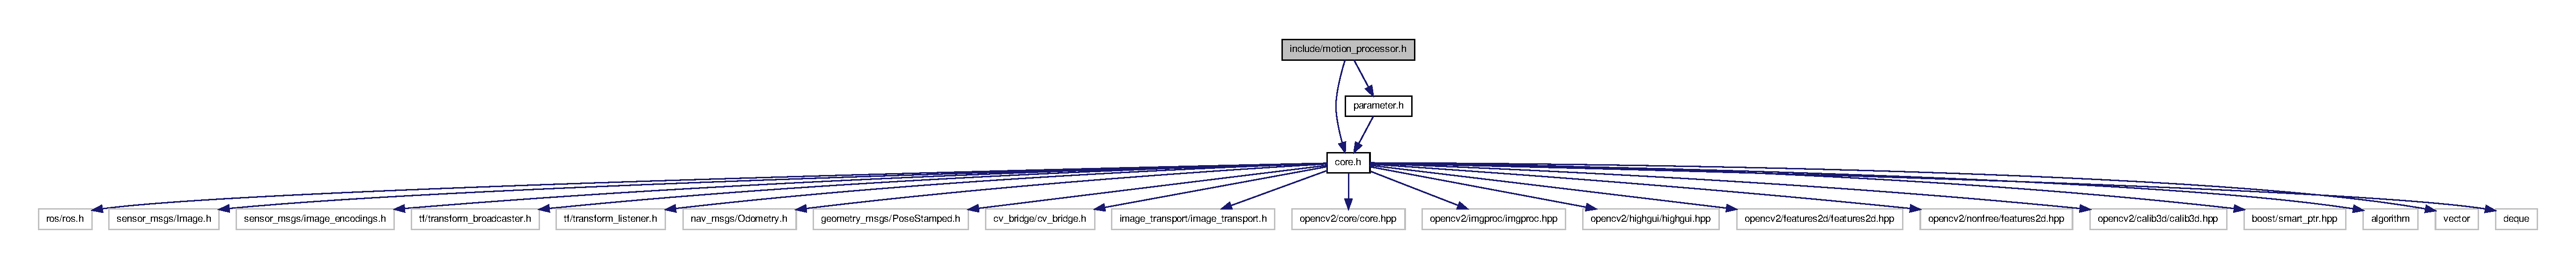
\includegraphics[width=350pt]{motion__processor_8h__incl}
\end{center}
\end{figure}
\-This graph shows which files directly or indirectly include this file\-:\nopagebreak
\begin{figure}[H]
\begin{center}
\leavevmode
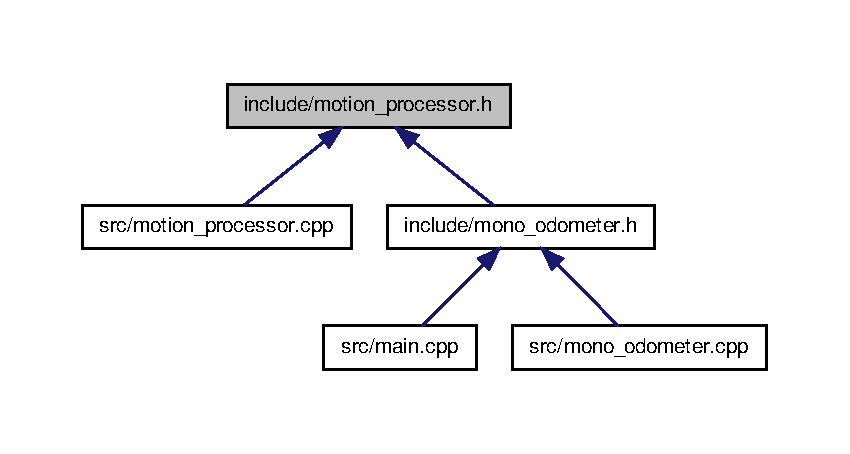
\includegraphics[width=350pt]{motion__processor_8h__dep__incl}
\end{center}
\end{figure}
\subsection*{\-Classes}
\begin{DoxyCompactItemize}
\item 
class \hyperlink{classLRM_1_1MotionProcessorParameter}{\-L\-R\-M\-::\-Motion\-Processor\-Parameter}
\item 
class \hyperlink{classLRM_1_1MotionProcessor}{\-L\-R\-M\-::\-Motion\-Processor}
\end{DoxyCompactItemize}
\subsection*{\-Namespaces}
\begin{DoxyCompactItemize}
\item 
namespace \hyperlink{namespaceLRM}{\-L\-R\-M}
\end{DoxyCompactItemize}

\hypertarget{parameter_8h}{\section{include/parameter.h \-File \-Reference}
\label{parameter_8h}\index{include/parameter.\-h@{include/parameter.\-h}}
}
{\ttfamily \#include \char`\"{}core.\-h\char`\"{}}\*
\-Include dependency graph for parameter.\-h\-:\nopagebreak
\begin{figure}[H]
\begin{center}
\leavevmode
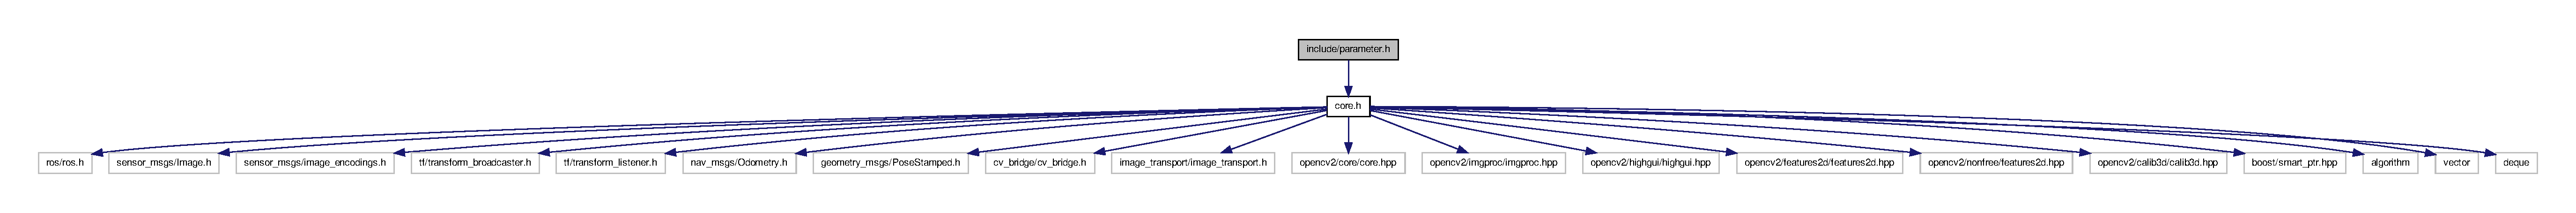
\includegraphics[width=350pt]{parameter_8h__incl}
\end{center}
\end{figure}
\-This graph shows which files directly or indirectly include this file\-:\nopagebreak
\begin{figure}[H]
\begin{center}
\leavevmode
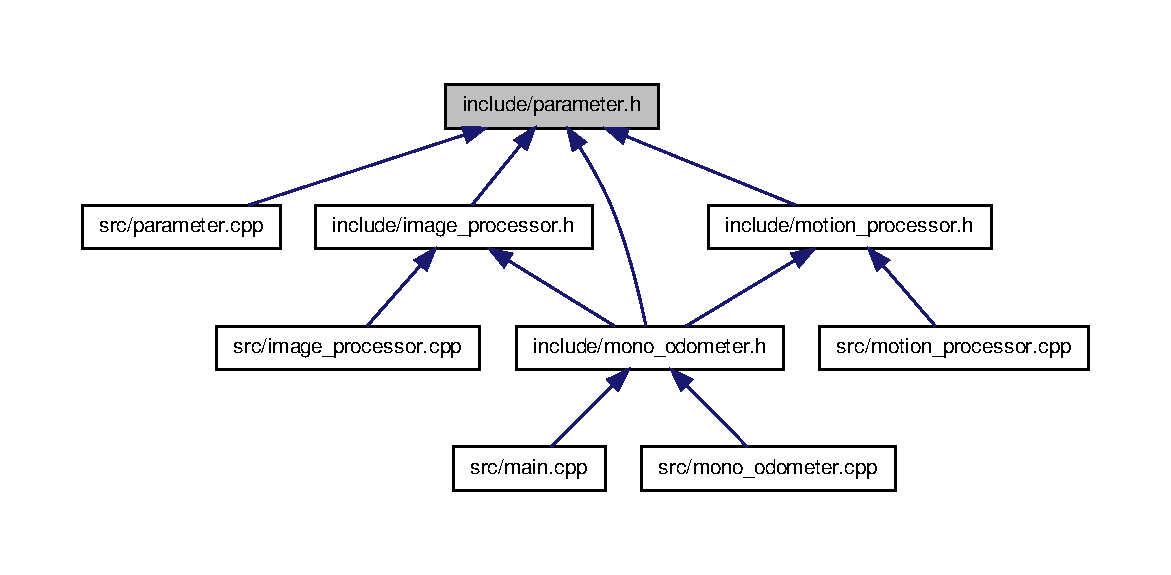
\includegraphics[width=350pt]{parameter_8h__dep__incl}
\end{center}
\end{figure}
\subsection*{\-Classes}
\begin{DoxyCompactItemize}
\item 
class \hyperlink{classLRM_1_1Parameter}{\-L\-R\-M\-::\-Parameter}
\end{DoxyCompactItemize}
\subsection*{\-Namespaces}
\begin{DoxyCompactItemize}
\item 
namespace \hyperlink{namespaceLRM}{\-L\-R\-M}
\end{DoxyCompactItemize}

\hypertarget{image__processor_8cpp}{\section{src/image\-\_\-processor.cpp \-File \-Reference}
\label{image__processor_8cpp}\index{src/image\-\_\-processor.\-cpp@{src/image\-\_\-processor.\-cpp}}
}
{\ttfamily \#include \char`\"{}image\-\_\-processor.\-h\char`\"{}}\*
\-Include dependency graph for image\-\_\-processor.\-cpp\-:\nopagebreak
\begin{figure}[H]
\begin{center}
\leavevmode
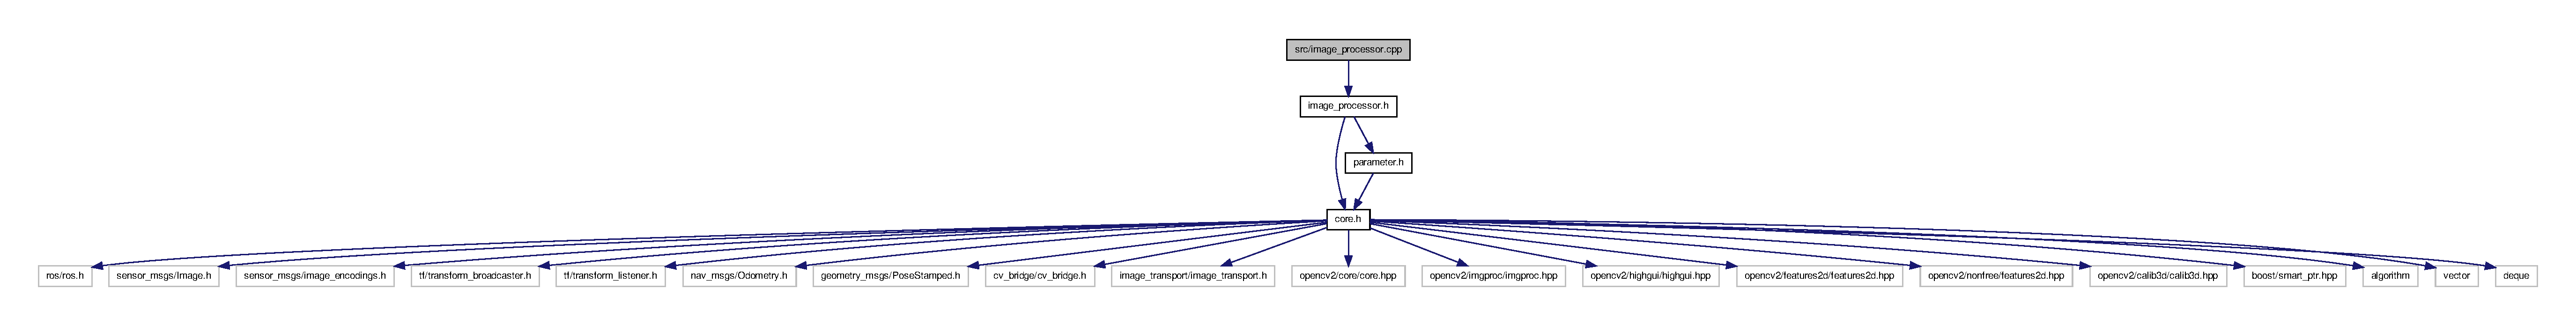
\includegraphics[width=350pt]{image__processor_8cpp__incl}
\end{center}
\end{figure}
\subsection*{\-Namespaces}
\begin{DoxyCompactItemize}
\item 
namespace \hyperlink{namespaceLRM}{\-L\-R\-M}
\end{DoxyCompactItemize}

\hypertarget{main_8cpp}{\section{src/main.cpp \-File \-Reference}
\label{main_8cpp}\index{src/main.\-cpp@{src/main.\-cpp}}
}
{\ttfamily \#include $<$ros/ros.\-h$>$}\*
{\ttfamily \#include \char`\"{}mono\-\_\-odometer.\-h\char`\"{}}\*
\-Include dependency graph for main.\-cpp\-:\nopagebreak
\begin{figure}[H]
\begin{center}
\leavevmode
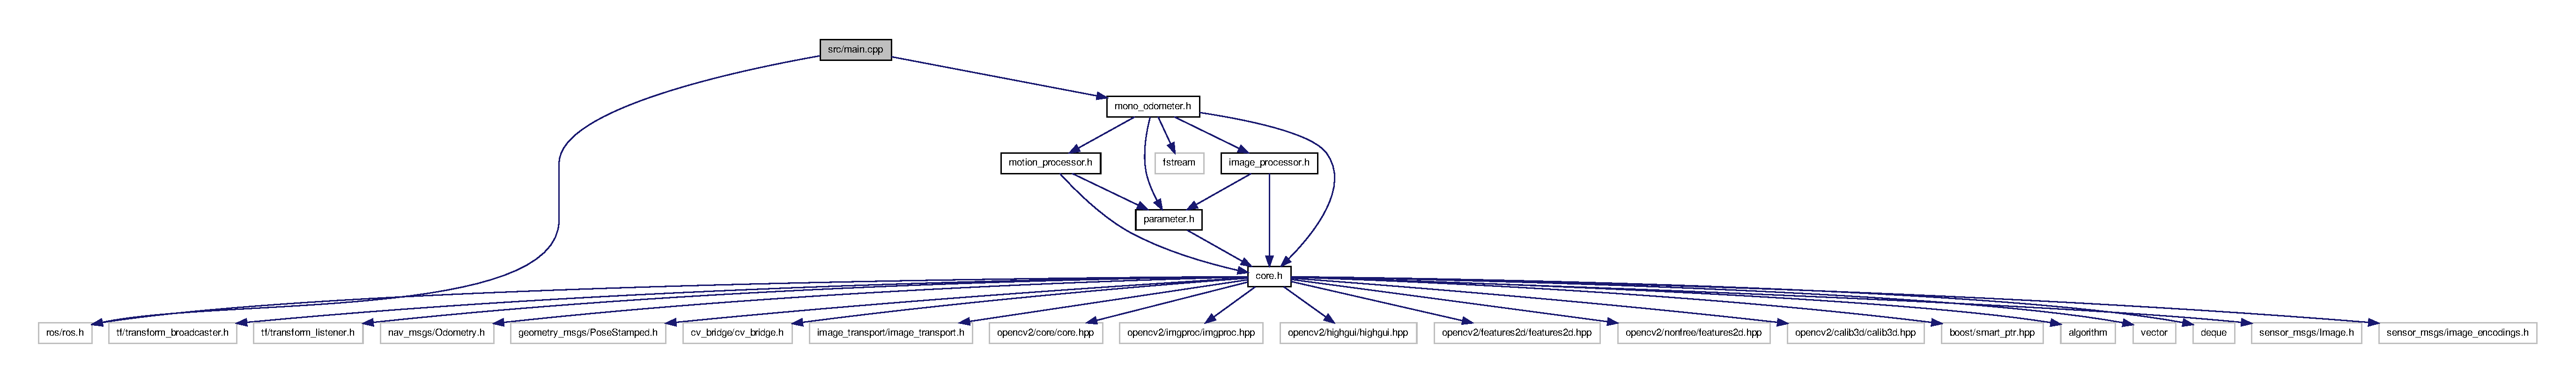
\includegraphics[width=350pt]{main_8cpp__incl}
\end{center}
\end{figure}
\subsection*{\-Functions}
\begin{DoxyCompactItemize}
\item 
int \hyperlink{main_8cpp_a3c04138a5bfe5d72780bb7e82a18e627}{main} (int argc, char $\ast$$\ast$argv)
\end{DoxyCompactItemize}


\subsection{\-Function \-Documentation}
\hypertarget{main_8cpp_a3c04138a5bfe5d72780bb7e82a18e627}{\index{main.\-cpp@{main.\-cpp}!main@{main}}
\index{main@{main}!main.cpp@{main.\-cpp}}
\subsubsection[{main}]{\setlength{\rightskip}{0pt plus 5cm}int {\bf main} (
\begin{DoxyParamCaption}
\item[{int}]{argc, }
\item[{char $\ast$$\ast$}]{argv}
\end{DoxyParamCaption}
)}}\label{main_8cpp_a3c04138a5bfe5d72780bb7e82a18e627}
\hyperlink{main_8cpp_a3c04138a5bfe5d72780bb7e82a18e627}{main()} 
\hypertarget{mono__odometer_8cpp}{\section{src/mono\-\_\-odometer.cpp \-File \-Reference}
\label{mono__odometer_8cpp}\index{src/mono\-\_\-odometer.\-cpp@{src/mono\-\_\-odometer.\-cpp}}
}
{\ttfamily \#include \char`\"{}mono\-\_\-odometer.\-h\char`\"{}}\*
\-Include dependency graph for mono\-\_\-odometer.\-cpp\-:\nopagebreak
\begin{figure}[H]
\begin{center}
\leavevmode
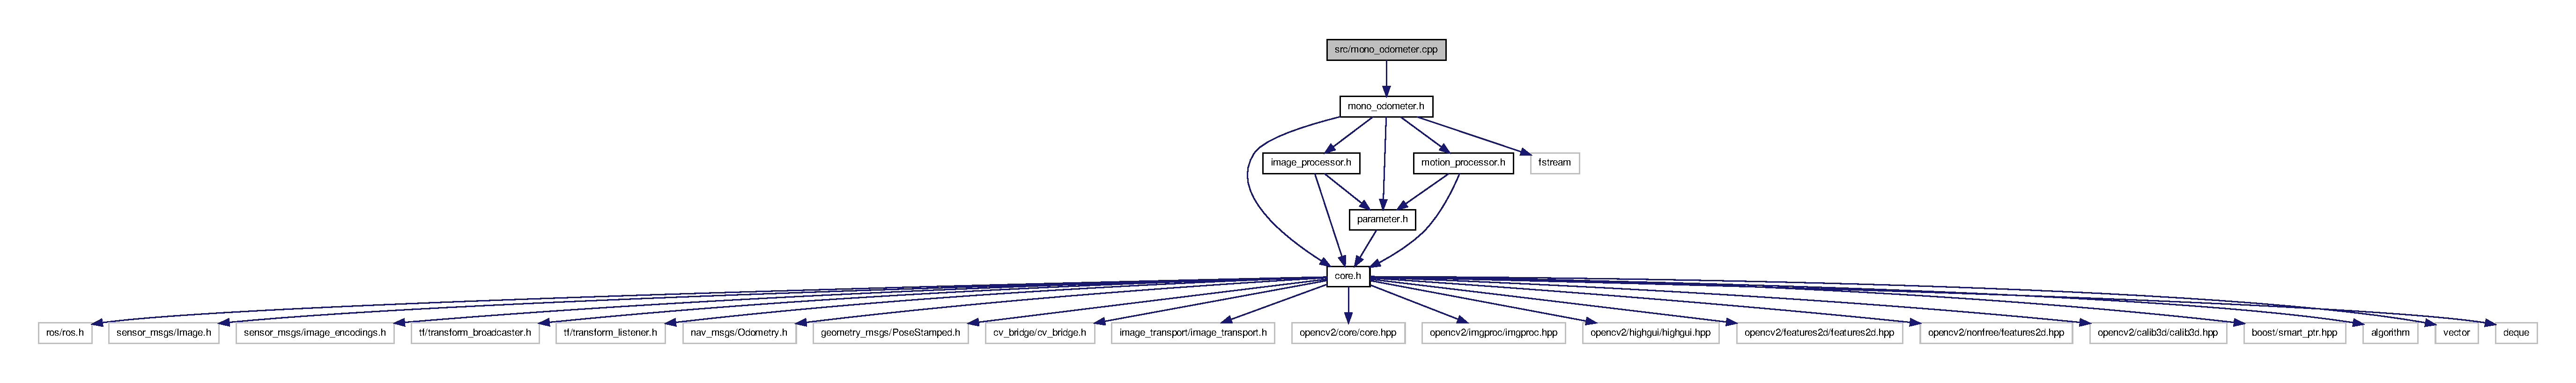
\includegraphics[width=350pt]{mono__odometer_8cpp__incl}
\end{center}
\end{figure}
\subsection*{\-Namespaces}
\begin{DoxyCompactItemize}
\item 
namespace \hyperlink{namespaceLRM}{\-L\-R\-M}
\end{DoxyCompactItemize}

\hypertarget{motion__processor_8cpp}{\section{src/motion\-\_\-processor.cpp \-File \-Reference}
\label{motion__processor_8cpp}\index{src/motion\-\_\-processor.\-cpp@{src/motion\-\_\-processor.\-cpp}}
}
{\ttfamily \#include \char`\"{}motion\-\_\-processor.\-h\char`\"{}}\*
\-Include dependency graph for motion\-\_\-processor.\-cpp\-:\nopagebreak
\begin{figure}[H]
\begin{center}
\leavevmode
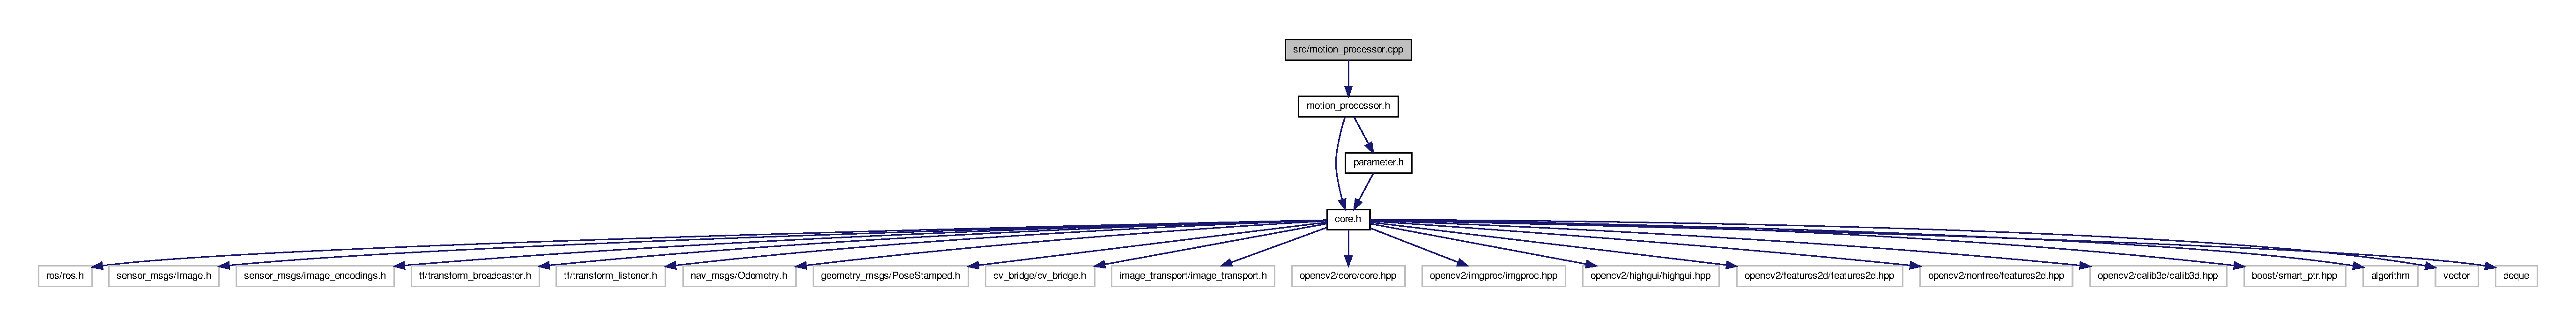
\includegraphics[width=350pt]{motion__processor_8cpp__incl}
\end{center}
\end{figure}
\subsection*{\-Namespaces}
\begin{DoxyCompactItemize}
\item 
namespace \hyperlink{namespaceLRM}{\-L\-R\-M}
\end{DoxyCompactItemize}

\hypertarget{parameter_8cpp}{\section{src/parameter.cpp \-File \-Reference}
\label{parameter_8cpp}\index{src/parameter.\-cpp@{src/parameter.\-cpp}}
}
{\ttfamily \#include \char`\"{}parameter.\-h\char`\"{}}\*
\-Include dependency graph for parameter.\-cpp\-:\nopagebreak
\begin{figure}[H]
\begin{center}
\leavevmode
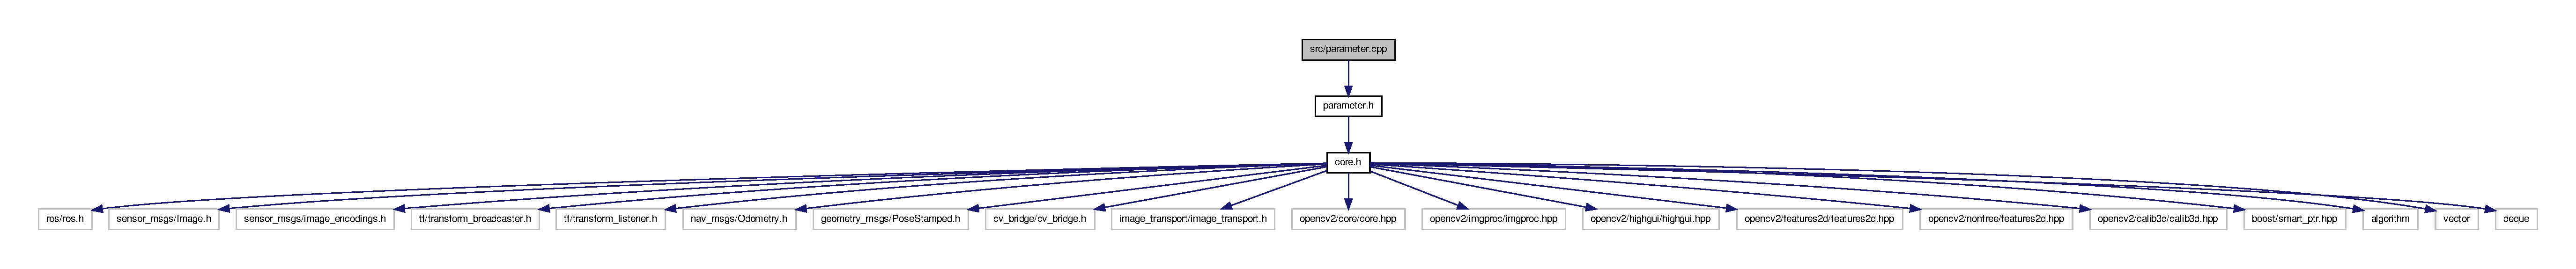
\includegraphics[width=350pt]{parameter_8cpp__incl}
\end{center}
\end{figure}
\subsection*{\-Namespaces}
\begin{DoxyCompactItemize}
\item 
namespace \hyperlink{namespaceLRM}{\-L\-R\-M}
\end{DoxyCompactItemize}

\printindex
\end{document}
